% Options for packages loaded elsewhere
\PassOptionsToPackage{unicode}{hyperref}
\PassOptionsToPackage{hyphens}{url}
\PassOptionsToPackage{dvipsnames,svgnames,x11names}{xcolor}
%
\documentclass[
  letterpaper,
  DIV=11,
  numbers=noendperiod]{scrartcl}

\usepackage{amsmath,amssymb}
\usepackage{iftex}
\ifPDFTeX
  \usepackage[T1]{fontenc}
  \usepackage[utf8]{inputenc}
  \usepackage{textcomp} % provide euro and other symbols
\else % if luatex or xetex
  \usepackage{unicode-math}
  \defaultfontfeatures{Scale=MatchLowercase}
  \defaultfontfeatures[\rmfamily]{Ligatures=TeX,Scale=1}
\fi
\usepackage{lmodern}
\ifPDFTeX\else  
    % xetex/luatex font selection
\fi
% Use upquote if available, for straight quotes in verbatim environments
\IfFileExists{upquote.sty}{\usepackage{upquote}}{}
\IfFileExists{microtype.sty}{% use microtype if available
  \usepackage[]{microtype}
  \UseMicrotypeSet[protrusion]{basicmath} % disable protrusion for tt fonts
}{}
\makeatletter
\@ifundefined{KOMAClassName}{% if non-KOMA class
  \IfFileExists{parskip.sty}{%
    \usepackage{parskip}
  }{% else
    \setlength{\parindent}{0pt}
    \setlength{\parskip}{6pt plus 2pt minus 1pt}}
}{% if KOMA class
  \KOMAoptions{parskip=half}}
\makeatother
\usepackage{xcolor}
\setlength{\emergencystretch}{3em} % prevent overfull lines
\setcounter{secnumdepth}{2}
% Make \paragraph and \subparagraph free-standing
\ifx\paragraph\undefined\else
  \let\oldparagraph\paragraph
  \renewcommand{\paragraph}[1]{\oldparagraph{#1}\mbox{}}
\fi
\ifx\subparagraph\undefined\else
  \let\oldsubparagraph\subparagraph
  \renewcommand{\subparagraph}[1]{\oldsubparagraph{#1}\mbox{}}
\fi

\usepackage{color}
\usepackage{fancyvrb}
\newcommand{\VerbBar}{|}
\newcommand{\VERB}{\Verb[commandchars=\\\{\}]}
\DefineVerbatimEnvironment{Highlighting}{Verbatim}{commandchars=\\\{\}}
% Add ',fontsize=\small' for more characters per line
\usepackage{framed}
\definecolor{shadecolor}{RGB}{241,243,245}
\newenvironment{Shaded}{\begin{snugshade}}{\end{snugshade}}
\newcommand{\AlertTok}[1]{\textcolor[rgb]{0.68,0.00,0.00}{#1}}
\newcommand{\AnnotationTok}[1]{\textcolor[rgb]{0.37,0.37,0.37}{#1}}
\newcommand{\AttributeTok}[1]{\textcolor[rgb]{0.40,0.45,0.13}{#1}}
\newcommand{\BaseNTok}[1]{\textcolor[rgb]{0.68,0.00,0.00}{#1}}
\newcommand{\BuiltInTok}[1]{\textcolor[rgb]{0.00,0.23,0.31}{#1}}
\newcommand{\CharTok}[1]{\textcolor[rgb]{0.13,0.47,0.30}{#1}}
\newcommand{\CommentTok}[1]{\textcolor[rgb]{0.37,0.37,0.37}{#1}}
\newcommand{\CommentVarTok}[1]{\textcolor[rgb]{0.37,0.37,0.37}{\textit{#1}}}
\newcommand{\ConstantTok}[1]{\textcolor[rgb]{0.56,0.35,0.01}{#1}}
\newcommand{\ControlFlowTok}[1]{\textcolor[rgb]{0.00,0.23,0.31}{#1}}
\newcommand{\DataTypeTok}[1]{\textcolor[rgb]{0.68,0.00,0.00}{#1}}
\newcommand{\DecValTok}[1]{\textcolor[rgb]{0.68,0.00,0.00}{#1}}
\newcommand{\DocumentationTok}[1]{\textcolor[rgb]{0.37,0.37,0.37}{\textit{#1}}}
\newcommand{\ErrorTok}[1]{\textcolor[rgb]{0.68,0.00,0.00}{#1}}
\newcommand{\ExtensionTok}[1]{\textcolor[rgb]{0.00,0.23,0.31}{#1}}
\newcommand{\FloatTok}[1]{\textcolor[rgb]{0.68,0.00,0.00}{#1}}
\newcommand{\FunctionTok}[1]{\textcolor[rgb]{0.28,0.35,0.67}{#1}}
\newcommand{\ImportTok}[1]{\textcolor[rgb]{0.00,0.46,0.62}{#1}}
\newcommand{\InformationTok}[1]{\textcolor[rgb]{0.37,0.37,0.37}{#1}}
\newcommand{\KeywordTok}[1]{\textcolor[rgb]{0.00,0.23,0.31}{#1}}
\newcommand{\NormalTok}[1]{\textcolor[rgb]{0.00,0.23,0.31}{#1}}
\newcommand{\OperatorTok}[1]{\textcolor[rgb]{0.37,0.37,0.37}{#1}}
\newcommand{\OtherTok}[1]{\textcolor[rgb]{0.00,0.23,0.31}{#1}}
\newcommand{\PreprocessorTok}[1]{\textcolor[rgb]{0.68,0.00,0.00}{#1}}
\newcommand{\RegionMarkerTok}[1]{\textcolor[rgb]{0.00,0.23,0.31}{#1}}
\newcommand{\SpecialCharTok}[1]{\textcolor[rgb]{0.37,0.37,0.37}{#1}}
\newcommand{\SpecialStringTok}[1]{\textcolor[rgb]{0.13,0.47,0.30}{#1}}
\newcommand{\StringTok}[1]{\textcolor[rgb]{0.13,0.47,0.30}{#1}}
\newcommand{\VariableTok}[1]{\textcolor[rgb]{0.07,0.07,0.07}{#1}}
\newcommand{\VerbatimStringTok}[1]{\textcolor[rgb]{0.13,0.47,0.30}{#1}}
\newcommand{\WarningTok}[1]{\textcolor[rgb]{0.37,0.37,0.37}{\textit{#1}}}

\providecommand{\tightlist}{%
  \setlength{\itemsep}{0pt}\setlength{\parskip}{0pt}}\usepackage{longtable,booktabs,array}
\usepackage{calc} % for calculating minipage widths
% Correct order of tables after \paragraph or \subparagraph
\usepackage{etoolbox}
\makeatletter
\patchcmd\longtable{\par}{\if@noskipsec\mbox{}\fi\par}{}{}
\makeatother
% Allow footnotes in longtable head/foot
\IfFileExists{footnotehyper.sty}{\usepackage{footnotehyper}}{\usepackage{footnote}}
\makesavenoteenv{longtable}
\usepackage{graphicx}
\makeatletter
\def\maxwidth{\ifdim\Gin@nat@width>\linewidth\linewidth\else\Gin@nat@width\fi}
\def\maxheight{\ifdim\Gin@nat@height>\textheight\textheight\else\Gin@nat@height\fi}
\makeatother
% Scale images if necessary, so that they will not overflow the page
% margins by default, and it is still possible to overwrite the defaults
% using explicit options in \includegraphics[width, height, ...]{}
\setkeys{Gin}{width=\maxwidth,height=\maxheight,keepaspectratio}
% Set default figure placement to htbp
\makeatletter
\def\fps@figure{htbp}
\makeatother

\KOMAoption{captions}{tableheading}
\usepackage{marginnote, here, relsize, needspace, setspace} \def\it{\emph}
\makeatletter
\@ifpackageloaded{caption}{}{\usepackage{caption}}
\AtBeginDocument{%
\ifdefined\contentsname
  \renewcommand*\contentsname{Table of contents}
\else
  \newcommand\contentsname{Table of contents}
\fi
\ifdefined\listfigurename
  \renewcommand*\listfigurename{List of Figures}
\else
  \newcommand\listfigurename{List of Figures}
\fi
\ifdefined\listtablename
  \renewcommand*\listtablename{List of Tables}
\else
  \newcommand\listtablename{List of Tables}
\fi
\ifdefined\figurename
  \renewcommand*\figurename{Figure}
\else
  \newcommand\figurename{Figure}
\fi
\ifdefined\tablename
  \renewcommand*\tablename{Table}
\else
  \newcommand\tablename{Table}
\fi
}
\@ifpackageloaded{float}{}{\usepackage{float}}
\floatstyle{ruled}
\@ifundefined{c@chapter}{\newfloat{codelisting}{h}{lop}}{\newfloat{codelisting}{h}{lop}[chapter]}
\floatname{codelisting}{Listing}
\newcommand*\listoflistings{\listof{codelisting}{List of Listings}}
\makeatother
\makeatletter
\makeatother
\makeatletter
\@ifpackageloaded{caption}{}{\usepackage{caption}}
\@ifpackageloaded{subcaption}{}{\usepackage{subcaption}}
\makeatother
\ifLuaTeX
  \usepackage{selnolig}  % disable illegal ligatures
\fi
\usepackage{bookmark}

\IfFileExists{xurl.sty}{\usepackage{xurl}}{} % add URL line breaks if available
\urlstyle{same} % disable monospaced font for URLs
\hypersetup{
  pdftitle={Lab: Bayes and Penguins},
  pdfauthor={KW},
  colorlinks=true,
  linkcolor={blue},
  filecolor={Maroon},
  citecolor={Blue},
  urlcolor={Blue},
  pdfcreator={LaTeX via pandoc}}

\title{Lab: Bayes and Penguins}
\usepackage{etoolbox}
\makeatletter
\providecommand{\subtitle}[1]{% add subtitle to \maketitle
  \apptocmd{\@title}{\par {\large #1 \par}}{}{}
}
\makeatother
\subtitle{Princeton University}
\author{KW}
\date{2025-04-02}

\begin{document}
\maketitle

Here is a worksheet and assignment that combines Bayes (brms) with
tidyverse tools. The focus is on the essentials when it comes to simple
linear regression with brms.

Please read and run through this worksheet and answer the conceptual
questions that are interleaved within them. At the end of each part, is
a coding exercise based on the material you've read until then.

\section{Part 1: EDA, OLS, BRMS}\label{part-1-eda-ols-brms}

\subsection{Packages and data}\label{packages-and-data}

Load the primary packages.

\begin{Shaded}
\begin{Highlighting}[]
\FunctionTok{library}\NormalTok{(tidyverse)}
\FunctionTok{library}\NormalTok{(ggside)}
\FunctionTok{library}\NormalTok{(brms)}
\FunctionTok{library}\NormalTok{(broom)}
\FunctionTok{library}\NormalTok{(broom.mixed)}
\end{Highlighting}
\end{Shaded}

We'll use the \texttt{penguins} data set from the
\textbf{palmerpenguins} package.

\begin{Shaded}
\begin{Highlighting}[]
\FunctionTok{data}\NormalTok{(penguins, }\AttributeTok{package =} \StringTok{"palmerpenguins"}\NormalTok{)}

\CommentTok{\# Any type of looking at data is a part of EDA }
\FunctionTok{glimpse}\NormalTok{(penguins)}
\end{Highlighting}
\end{Shaded}

\begin{verbatim}
Rows: 344
Columns: 8
$ species           <fct> Adelie, Adelie, Adelie, Adelie, Adelie, Adelie, Adel~
$ island            <fct> Torgersen, Torgersen, Torgersen, Torgersen, Torgerse~
$ bill_length_mm    <dbl> 39.1, 39.5, 40.3, NA, 36.7, 39.3, 38.9, 39.2, 34.1, ~
$ bill_depth_mm     <dbl> 18.7, 17.4, 18.0, NA, 19.3, 20.6, 17.8, 19.6, 18.1, ~
$ flipper_length_mm <int> 181, 186, 195, NA, 193, 190, 181, 195, 193, 190, 186~
$ body_mass_g       <int> 3750, 3800, 3250, NA, 3450, 3650, 3625, 4675, 3475, ~
$ sex               <fct> male, female, female, NA, female, male, female, male~
$ year              <int> 2007, 2007, 2007, 2007, 2007, 2007, 2007, 2007, 2007~
\end{verbatim}

\begin{Shaded}
\begin{Highlighting}[]
\FunctionTok{head}\NormalTok{(penguins)}
\end{Highlighting}
\end{Shaded}

\begin{verbatim}
# A tibble: 6 x 8
  species island    bill_length_mm bill_depth_mm flipper_length_mm body_mass_g
  <fct>   <fct>              <dbl>         <dbl>             <int>       <int>
1 Adelie  Torgersen           39.1          18.7               181        3750
2 Adelie  Torgersen           39.5          17.4               186        3800
3 Adelie  Torgersen           40.3          18                 195        3250
4 Adelie  Torgersen           NA            NA                  NA          NA
5 Adelie  Torgersen           36.7          19.3               193        3450
6 Adelie  Torgersen           39.3          20.6               190        3650
# i 2 more variables: sex <fct>, year <int>
\end{verbatim}

You might divide the data set by the three levels of \texttt{species}.

\begin{Shaded}
\begin{Highlighting}[]
\NormalTok{penguins }\SpecialCharTok{\%\textgreater{}\%} 
  \FunctionTok{count}\NormalTok{(species)}
\end{Highlighting}
\end{Shaded}

\begin{verbatim}
# A tibble: 3 x 2
  species       n
  <fct>     <int>
1 Adelie      152
2 Chinstrap    68
3 Gentoo      124
\end{verbatim}

To start, we'll make a subset of the data called \texttt{chinstrap}.

\begin{Shaded}
\begin{Highlighting}[]
\NormalTok{chinstrap }\OtherTok{\textless{}{-}}\NormalTok{ penguins }\SpecialCharTok{\%\textgreater{}\%} 
  \FunctionTok{filter}\NormalTok{(species }\SpecialCharTok{==} \StringTok{"Chinstrap"}\NormalTok{)}

\FunctionTok{glimpse}\NormalTok{(chinstrap)}
\end{Highlighting}
\end{Shaded}

\begin{verbatim}
Rows: 68
Columns: 8
$ species           <fct> Chinstrap, Chinstrap, Chinstrap, Chinstrap, Chinstra~
$ island            <fct> Dream, Dream, Dream, Dream, Dream, Dream, Dream, Dre~
$ bill_length_mm    <dbl> 46.5, 50.0, 51.3, 45.4, 52.7, 45.2, 46.1, 51.3, 46.0~
$ bill_depth_mm     <dbl> 17.9, 19.5, 19.2, 18.7, 19.8, 17.8, 18.2, 18.2, 18.9~
$ flipper_length_mm <int> 192, 196, 193, 188, 197, 198, 178, 197, 195, 198, 19~
$ body_mass_g       <int> 3500, 3900, 3650, 3525, 3725, 3950, 3250, 3750, 4150~
$ sex               <fct> female, male, male, female, male, female, female, ma~
$ year              <int> 2007, 2007, 2007, 2007, 2007, 2007, 2007, 2007, 2007~
\end{verbatim}

We've done from a full data set with \(N = 344\) rows, to a subset with
\(n = 68\) rows. (``\$'' signs hold LaTex snippets)

\subsection{More Exploratory data analysis
(EDA)}\label{more-exploratory-data-analysis-eda}

Our focal variables will be \texttt{body\_mass\_g} and
\texttt{bill\_length\_mm}. Here they are in a scatter plot.

\begin{Shaded}
\begin{Highlighting}[]
\NormalTok{chinstrap }\SpecialCharTok{\%\textgreater{}\%} 
  \FunctionTok{ggplot}\NormalTok{(}\FunctionTok{aes}\NormalTok{(}\AttributeTok{x =}\NormalTok{ body\_mass\_g, }\AttributeTok{y =}\NormalTok{ bill\_length\_mm)) }\SpecialCharTok{+}
  \FunctionTok{geom\_point}\NormalTok{() }\SpecialCharTok{+}
  \FunctionTok{stat\_smooth}\NormalTok{(}\AttributeTok{method =} \StringTok{"lm"}\NormalTok{, }\AttributeTok{formula =} \StringTok{\textquotesingle{}y \textasciitilde{} x\textquotesingle{}}\NormalTok{, }\AttributeTok{se =} \ConstantTok{FALSE}\NormalTok{)}
\end{Highlighting}
\end{Shaded}

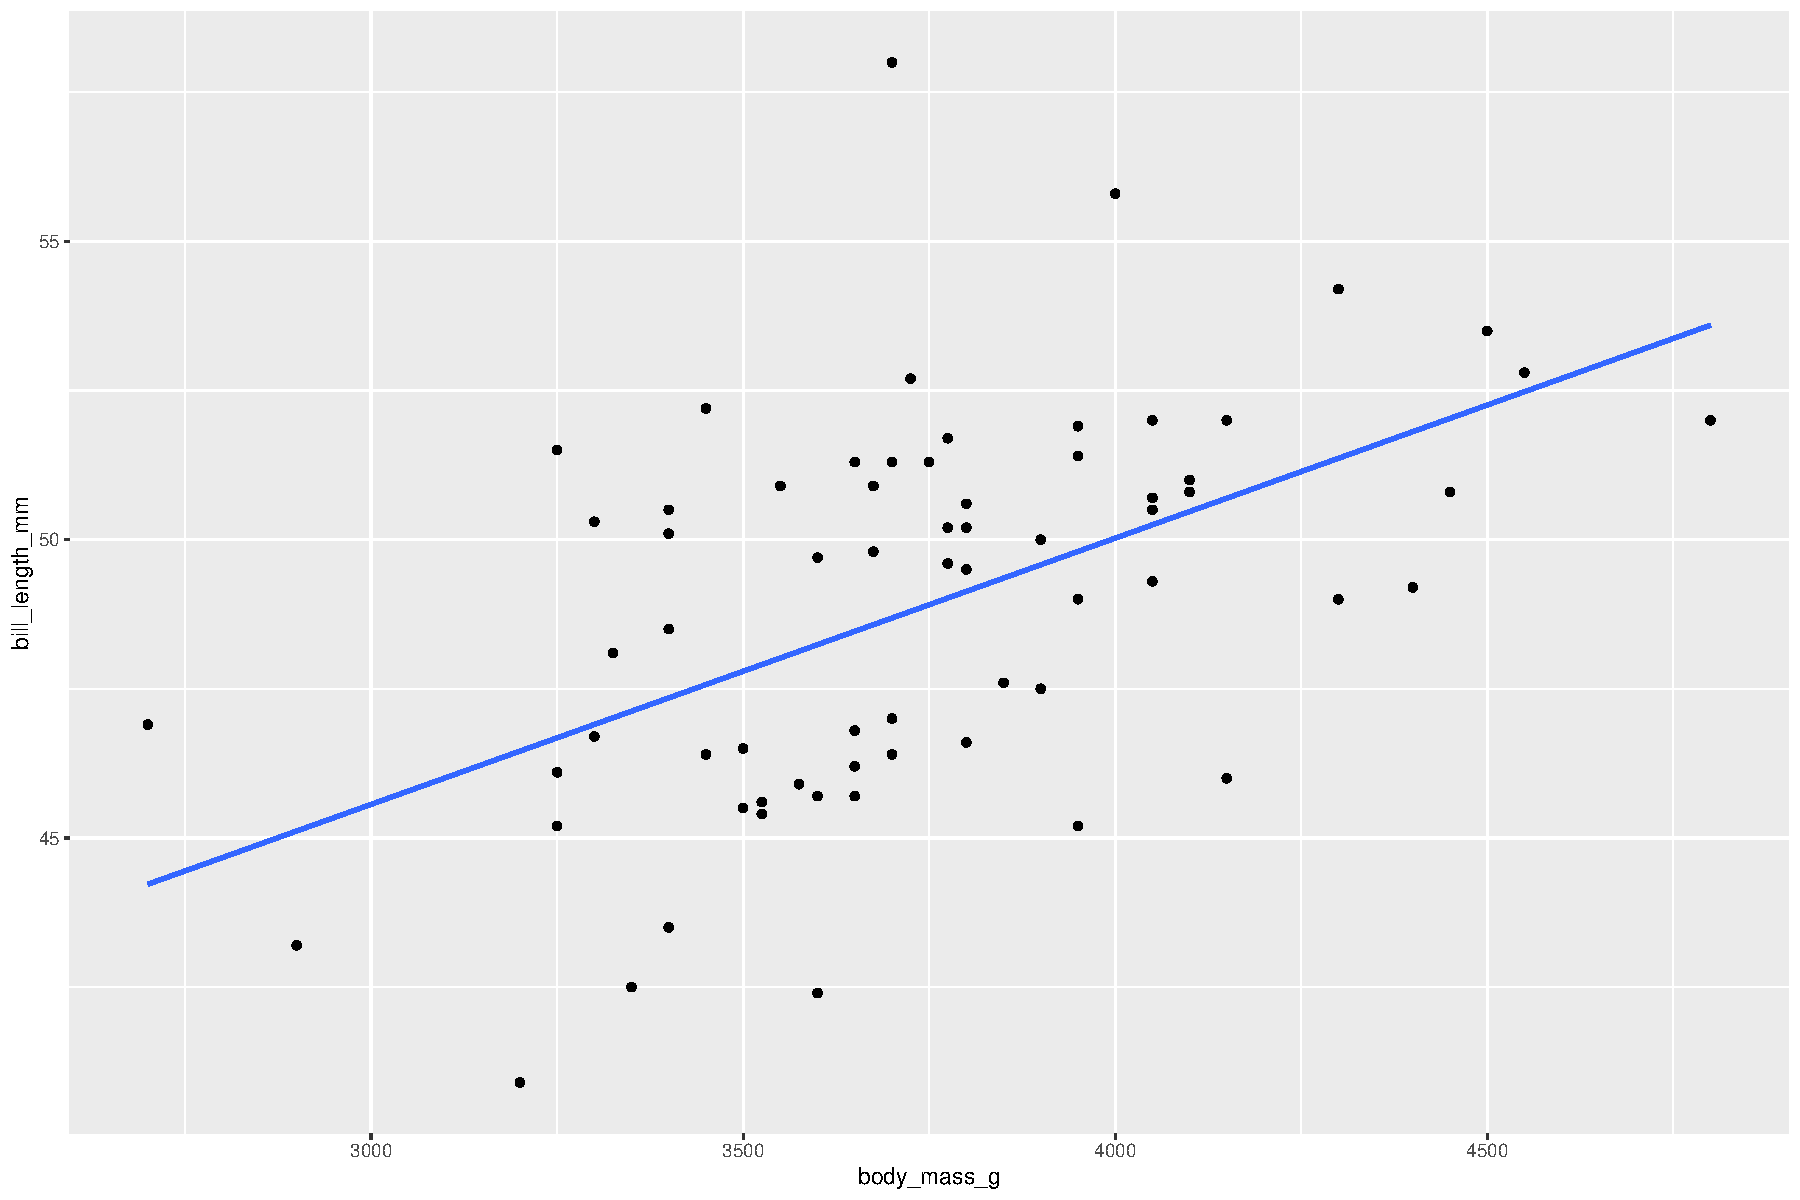
\includegraphics{Bayes_Lab_1_files/figure-pdf/unnamed-chunk-5-1.pdf}

We can augment the plot with some nice functions from the
\textbf{ggside} package.

\begin{Shaded}
\begin{Highlighting}[]
\NormalTok{chinstrap }\SpecialCharTok{\%\textgreater{}\%} 
  \FunctionTok{ggplot}\NormalTok{(}\FunctionTok{aes}\NormalTok{(}\AttributeTok{x =}\NormalTok{ body\_mass\_g, }\AttributeTok{y =}\NormalTok{ bill\_length\_mm)) }\SpecialCharTok{+}
  \FunctionTok{geom\_point}\NormalTok{() }\SpecialCharTok{+}
  \FunctionTok{stat\_smooth}\NormalTok{(}\AttributeTok{method =} \StringTok{"lm"}\NormalTok{, }\AttributeTok{formula =} \StringTok{\textquotesingle{}y \textasciitilde{} x\textquotesingle{}}\NormalTok{, }\AttributeTok{se =} \ConstantTok{FALSE}\NormalTok{) }\SpecialCharTok{+}
  \CommentTok{\# from ggside}
  \FunctionTok{geom\_xsidehistogram}\NormalTok{(}\AttributeTok{bins =} \DecValTok{30}\NormalTok{) }\SpecialCharTok{+}
  \FunctionTok{geom\_ysidehistogram}\NormalTok{(}\AttributeTok{bins =} \DecValTok{30}\NormalTok{) }\SpecialCharTok{+}
  \FunctionTok{scale\_xsidey\_continuous}\NormalTok{(}\AttributeTok{breaks =} \ConstantTok{NULL}\NormalTok{) }\SpecialCharTok{+}
  \FunctionTok{scale\_ysidex\_continuous}\NormalTok{(}\AttributeTok{breaks =} \ConstantTok{NULL}\NormalTok{) }\SpecialCharTok{+}
  \FunctionTok{theme}\NormalTok{(}\AttributeTok{ggside.panel.scale =} \FloatTok{0.25}\NormalTok{)}
\end{Highlighting}
\end{Shaded}

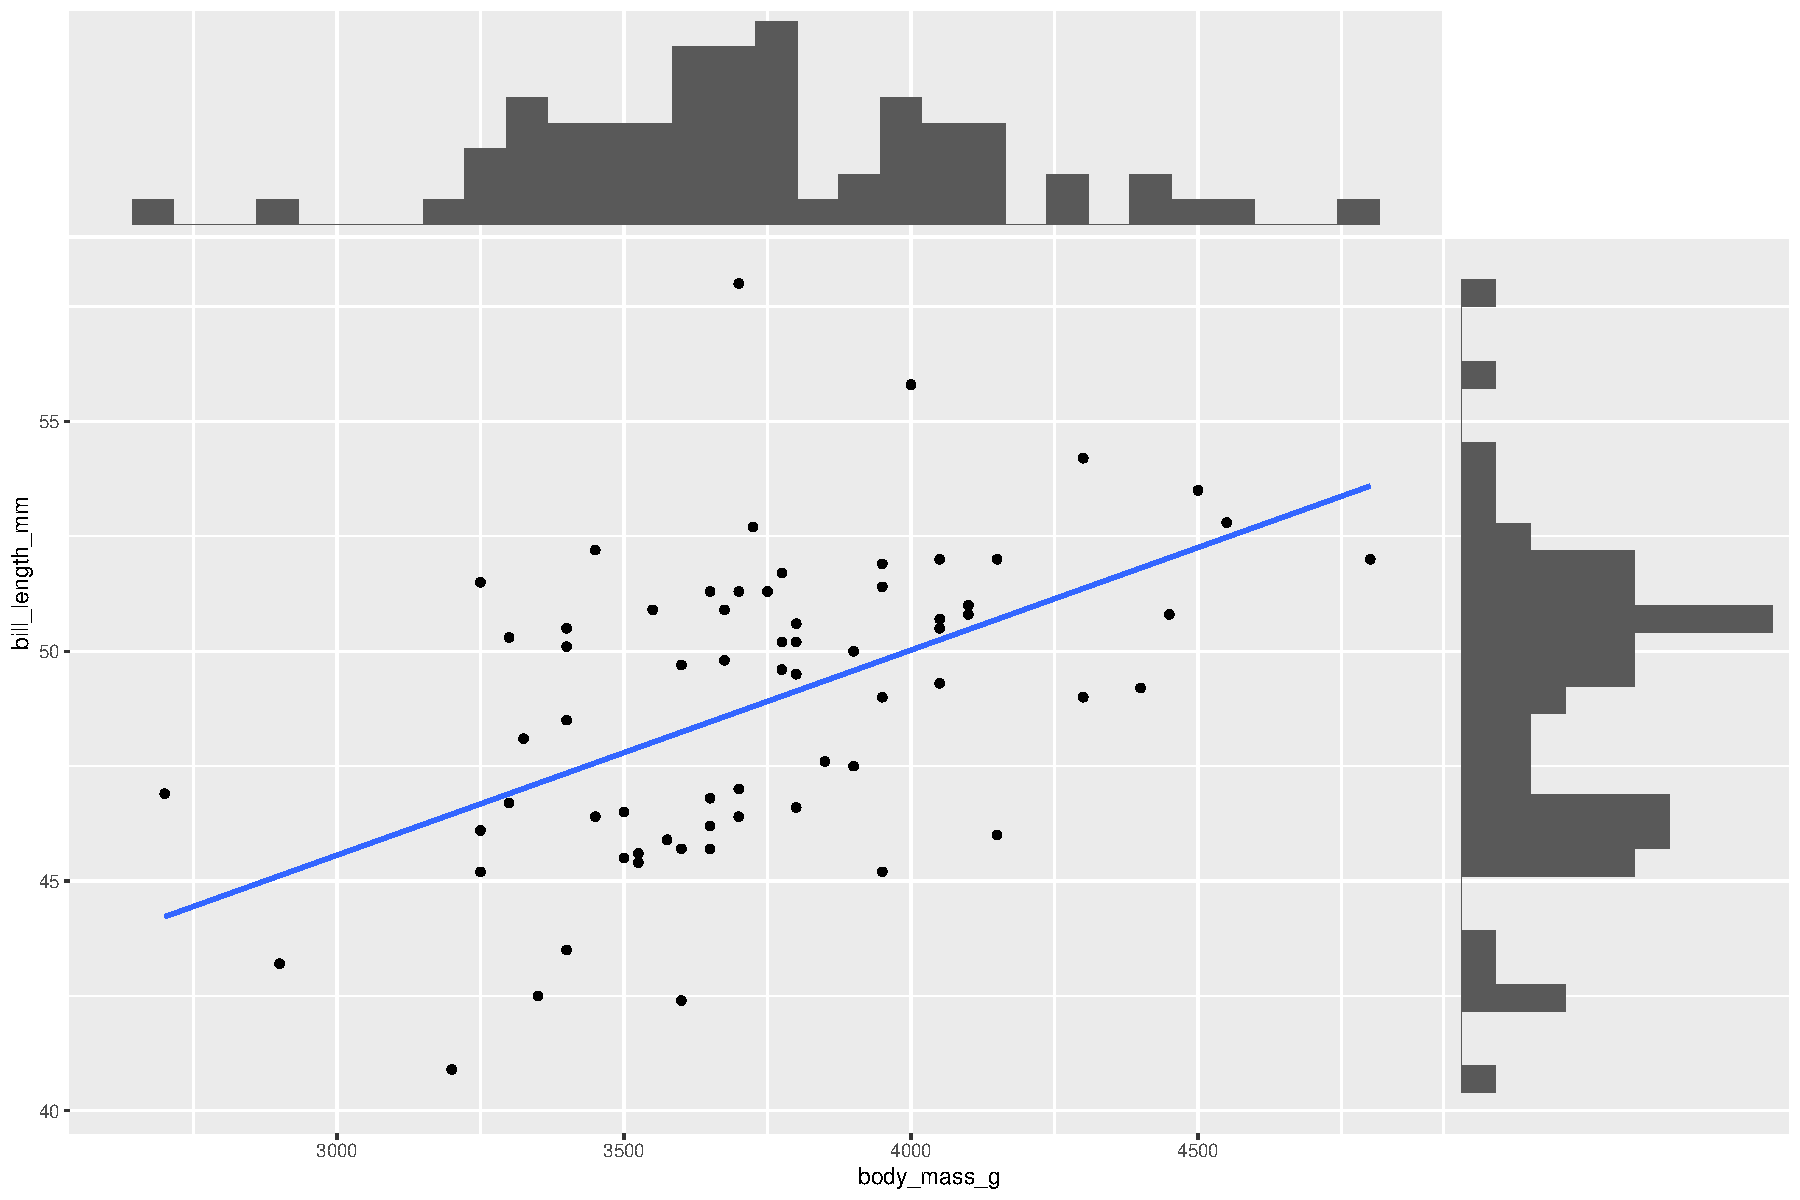
\includegraphics{Bayes_Lab_1_files/figure-pdf/unnamed-chunk-6-1.pdf}

It's a good idea to get a sense of the sample statistics. Here are the
means and SD's for the two variables.

\begin{Shaded}
\begin{Highlighting}[]
\NormalTok{chinstrap }\SpecialCharTok{\%\textgreater{}\%} 
  \FunctionTok{summarise}\NormalTok{(}\AttributeTok{body\_mass\_g\_mean =} \FunctionTok{mean}\NormalTok{(body\_mass\_g),}
            \AttributeTok{body\_mass\_g\_sd =} \FunctionTok{sd}\NormalTok{(body\_mass\_g),}
            \AttributeTok{bill\_length\_mm\_mean =} \FunctionTok{mean}\NormalTok{(bill\_length\_mm),}
            \AttributeTok{bill\_length\_mm\_sd =} \FunctionTok{sd}\NormalTok{(bill\_length\_mm)) }
\end{Highlighting}
\end{Shaded}

\begin{verbatim}
# A tibble: 1 x 4
  body_mass_g_mean body_mass_g_sd bill_length_mm_mean bill_length_mm_sd
             <dbl>          <dbl>               <dbl>             <dbl>
1            3733.           384.                48.8              3.34
\end{verbatim}

And you know that more efficient way to compute sample statistics for
multiple variables is to first convert the data into the long format
with \texttt{pivot\_longer()}. Then you use a \texttt{group\_by()} line
before the main event in \texttt{summarise()}.

\begin{Shaded}
\begin{Highlighting}[]
\NormalTok{chinstrap }\SpecialCharTok{\%\textgreater{}\%} 
  \FunctionTok{pivot\_longer}\NormalTok{(}\AttributeTok{cols =} \FunctionTok{c}\NormalTok{(body\_mass\_g, bill\_length\_mm)) }\SpecialCharTok{\%\textgreater{}\%} 
  \FunctionTok{group\_by}\NormalTok{(name) }\SpecialCharTok{\%\textgreater{}\%} 
  \FunctionTok{summarise}\NormalTok{(}\AttributeTok{mean =} \FunctionTok{mean}\NormalTok{(value),}
            \AttributeTok{sd =} \FunctionTok{sd}\NormalTok{(value),}
            \CommentTok{\# count the missing data (if any)}
            \AttributeTok{n\_missing =} \FunctionTok{sum}\NormalTok{(}\FunctionTok{is.na}\NormalTok{(value))) }
\end{Highlighting}
\end{Shaded}

\begin{verbatim}
# A tibble: 2 x 4
  name             mean     sd n_missing
  <chr>           <dbl>  <dbl>     <int>
1 bill_length_mm   48.8   3.34         0
2 body_mass_g    3733.  384.           0
\end{verbatim}

\subsubsection{Question 1.1: What do the marginal histograms added by
ggside tell you about the distribution of body\_mass\_g and
bill\_length\_mm
individually?}\label{question-1.1-what-do-the-marginal-histograms-added-by-ggside-tell-you-about-the-distribution-of-body_mass_g-and-bill_length_mm-individually}

\begin{verbatim}
The distribution of body_mass_g and bill_length_mm are probably not gaussian. They both look kinda bimodal.
\end{verbatim}

\subsection{OLS}\label{ols}

We'll fit the model

\$\$ \begin{align}

\text{bill_length_mm}\_i &= \beta_0 + \beta_1 \text{body_mass_g}\_i + \epsilon_i \\

\epsilon_i &\sim \operatorname{Normal}(0, \sigma\_\epsilon) \\

\end{align}

\$\$

where \texttt{bill\_length\_mm} is the \emph{dependent} variable or a
\emph{response} variable. The sole predictor is \texttt{body\_mass\_g}.
Both variables have \(i\) subscripts, which indicate they vary across
the \(i\) rows in the data set. For now, you might think if \(i\) as
standing for ``index.'' The last term in the first line, \(\epsilon\),
is often called the \emph{error}, or \emph{noise} term. In the second
line, we see we're making the conventional assumption the ``errors'' are
normally distributed around the regression line.

An alternative and equivalent way to write that equation is

\$\$ \begin{align}

\text{bill_length_mm}_i &\sim \operatorname{Normal}(\mu_i, \sigma) \\
\mu_i &= \beta_0 + \beta_1 \text{body_mass_g}_i

\end{align} \$\$

which is meant to convey we are modeling \texttt{bill\_length\_mm} as
normally distributed, with a conditional mean. You don't tend to see
equations written this way in the OLS paradigm. However, this style of
notation will serve us better when we start modeling our data with other
distributions.

This notation grows on you

Fitting the model with the base \textbf{R} \texttt{lm()} function, which
uses the OLS algorithm.

\begin{Shaded}
\begin{Highlighting}[]
\CommentTok{\# fit}
\NormalTok{fit1.ols }\OtherTok{\textless{}{-}} \FunctionTok{lm}\NormalTok{(}
  \AttributeTok{data =}\NormalTok{ chinstrap,}
\NormalTok{  bill\_length\_mm }\SpecialCharTok{\textasciitilde{}} \DecValTok{1} \SpecialCharTok{+}\NormalTok{ body\_mass\_g}
\NormalTok{)}

\CommentTok{\# summarize the results}
\FunctionTok{summary}\NormalTok{(fit1.ols)}
\end{Highlighting}
\end{Shaded}

\begin{verbatim}

Call:
lm(formula = bill_length_mm ~ 1 + body_mass_g, data = chinstrap)

Residuals:
    Min      1Q  Median      3Q     Max 
-5.8399 -2.2370  0.3247  1.8385  9.3138 

Coefficients:
             Estimate Std. Error t value Pr(>|t|)    
(Intercept) 3.217e+01  3.443e+00   9.344 1.07e-13 ***
body_mass_g 4.463e-03  9.176e-04   4.863 7.48e-06 ***
---
Signif. codes:  0 '***' 0.001 '**' 0.01 '*' 0.05 '.' 0.1 ' ' 1

Residual standard error: 2.887 on 66 degrees of freedom
Multiple R-squared:  0.2638,    Adjusted R-squared:  0.2527 
F-statistic: 23.65 on 1 and 66 DF,  p-value: 7.48e-06
\end{verbatim}

The point estimates are in scientific notation. We can pull them with
the \texttt{coef()} function.

\begin{Shaded}
\begin{Highlighting}[]
\FunctionTok{coef}\NormalTok{(fit1.ols)}
\end{Highlighting}
\end{Shaded}

\begin{verbatim}
 (Intercept)  body_mass_g 
32.174192865  0.004462694 
\end{verbatim}

We can compute fitted values, or predictions, with the
\texttt{predict()} function. Here's the default behavior.

\begin{Shaded}
\begin{Highlighting}[]
\FunctionTok{predict}\NormalTok{(fit1.ols)}
\end{Highlighting}
\end{Shaded}

\begin{verbatim}
       1        2        3        4        5        6        7        8 
47.79362 49.57870 48.46303 47.90519 48.79773 49.80183 46.67795 48.90930 
       9       10       11       12       13       14       15       16 
50.69437 48.68616 49.13243 49.02086 48.68616 50.24810 48.12832 50.24810 
      17       18       19       20       21       22       23       24 
46.90108 48.68616 47.57049 51.81005 48.23989 47.34735 45.11601 49.13243 
      25       26       27       28       29       30       31       32 
46.90108 50.69437 47.34735 49.13243 48.68616 52.47945 46.45481 51.36378 
      33       34       35       36       37       38       39       40 
47.12422 50.47124 48.23989 49.57870 49.35556 53.59512 44.22347 52.25632 
      41       42       43       44       45       46       47       48 
49.80183 48.46303 48.01676 47.79362 48.57459 52.03318 47.34735 51.36378 
      49       50       51       52       53       54       55       56 
46.67795 48.57459 47.01265 49.80183 48.23989 50.24810 47.12422 47.57049 
      57       58       59       60       61       62       63       64 
46.67795 50.24810 49.13243 47.90519 49.80183 48.46303 48.46303 50.02497 
      65       66       67       68 
47.34735 49.02086 50.47124 49.02086 
\end{verbatim}

We get one prediction, one fitted value, for each case in the data set.
We can express the uncertainty around those predictions with confidence
intervals.

\begin{Shaded}
\begin{Highlighting}[]
\FunctionTok{predict}\NormalTok{(fit1.ols,}
        \AttributeTok{interval =} \StringTok{"confidence"}\NormalTok{) }\SpecialCharTok{\%\textgreater{}\%} 
  \CommentTok{\# just the top 6}
  \FunctionTok{head}\NormalTok{()}
\end{Highlighting}
\end{Shaded}

\begin{verbatim}
       fit      lwr      upr
1 47.79362 46.97456 48.61268
2 49.57870 48.81580 50.34160
3 48.46303 47.74771 49.17834
4 47.90519 47.10905 48.70133
5 48.79773 48.09864 49.49682
6 49.80183 48.99783 50.60584
\end{verbatim}

We might also ask for a standard error for each prediction.

\begin{Shaded}
\begin{Highlighting}[]
\FunctionTok{predict}\NormalTok{(fit1.ols,}
        \AttributeTok{se.fit =} \ConstantTok{TRUE}\NormalTok{) }\SpecialCharTok{\%\textgreater{}\%} 
  \FunctionTok{data.frame}\NormalTok{()}
\end{Highlighting}
\end{Shaded}

\begin{verbatim}
        fit    se.fit df residual.scale
1  47.79362 0.4102359 66       2.886728
2  49.57870 0.3821060 66       2.886728
3  48.46303 0.3582736 66       2.886728
4  47.90519 0.3987564 66       2.886728
5  48.79773 0.3501459 66       2.886728
6  49.80183 0.4026961 66       2.886728
7  46.67795 0.5648454 66       2.886728
8  48.90930 0.3504110 66       2.886728
9  50.69437 0.5185569 66       2.886728
10 48.68616 0.3513814 66       2.886728
11 49.13243 0.3554108 66       2.886728
12 49.02086 0.3521734 66       2.886728
13 48.68616 0.3513814 66       2.886728
14 50.24810 0.4550963 66       2.886728
15 48.12832 0.3789333 66       2.886728
16 50.24810 0.4550963 66       2.886728
17 46.90108 0.5296025 66       2.886728
18 48.68616 0.3513814 66       2.886728
19 47.57049 0.4359183 66       2.886728
20 51.81005 0.7050167 66       2.886728
21 48.23989 0.3707575 66       2.886728
22 47.34735 0.4647215 66       2.886728
23 45.11601 0.8407923 66       2.886728
24 49.13243 0.3554108 66       2.886728
25 46.90108 0.5296025 66       2.886728
26 50.69437 0.5185569 66       2.886728
27 47.34735 0.4647215 66       2.886728
28 49.13243 0.3554108 66       2.886728
29 48.68616 0.3513814 66       2.886728
30 52.47945 0.8273195 66       2.886728
31 46.45481 0.6015246 66       2.886728
32 51.36378 0.6270243 66       2.886728
33 47.12422 0.4961023 66       2.886728
34 50.47124 0.4856973 66       2.886728
35 48.23989 0.3707575 66       2.886728
36 49.57870 0.3821060 66       2.886728
37 49.35556 0.3661365 66       2.886728
38 53.59512 1.0397147 66       2.886728
39 44.22347 1.0105441 66       2.886728
40 52.25632 0.7859885 66       2.886728
41 49.80183 0.4026961 66       2.886728
42 48.46303 0.3582736 66       2.886728
43 48.01676 0.3882941 66       2.886728
44 47.79362 0.4102359 66       2.886728
45 48.57459 0.3541019 66       2.886728
46 52.03318 0.7451900 66       2.886728
47 47.34735 0.4647215 66       2.886728
48 51.36378 0.6270243 66       2.886728
49 46.67795 0.5648454 66       2.886728
50 48.57459 0.3541019 66       2.886728
51 47.01265 0.5126128 66       2.886728
52 49.80183 0.4026961 66       2.886728
53 48.23989 0.3707575 66       2.886728
54 50.24810 0.4550963 66       2.886728
55 47.12422 0.4961023 66       2.886728
56 47.57049 0.4359183 66       2.886728
57 46.67795 0.5648454 66       2.886728
58 50.24810 0.4550963 66       2.886728
59 49.13243 0.3554108 66       2.886728
60 47.90519 0.3987564 66       2.886728
61 49.80183 0.4026961 66       2.886728
62 48.46303 0.3582736 66       2.886728
63 48.46303 0.3582736 66       2.886728
64 50.02497 0.4272392 66       2.886728
65 47.34735 0.4647215 66       2.886728
66 49.02086 0.3521734 66       2.886728
67 50.47124 0.4856973 66       2.886728
68 49.02086 0.3521734 66       2.886728
\end{verbatim}

Instead of relying on predictions from the values in the data, we might
instead define a sequence of values from the predictor variable. We'll
call those \texttt{nd}.

\begin{Shaded}
\begin{Highlighting}[]
\NormalTok{nd }\OtherTok{\textless{}{-}} \FunctionTok{tibble}\NormalTok{(}\AttributeTok{body\_mass\_g =} \FunctionTok{seq}\NormalTok{(}\AttributeTok{from =} \FunctionTok{min}\NormalTok{(chinstrap}\SpecialCharTok{$}\NormalTok{body\_mass\_g),}
                               \AttributeTok{to =} \FunctionTok{max}\NormalTok{(chinstrap}\SpecialCharTok{$}\NormalTok{body\_mass\_g),}
                               \AttributeTok{length.out =} \DecValTok{50}\NormalTok{))}

\FunctionTok{glimpse}\NormalTok{(nd)}
\end{Highlighting}
\end{Shaded}

\begin{verbatim}
Rows: 50
Columns: 1
$ body_mass_g <dbl> 2700.000, 2742.857, 2785.714, 2828.571, 2871.429, 2914.286~
\end{verbatim}

We can insert our \texttt{nd} data into the \texttt{newdata} argument.

\begin{Shaded}
\begin{Highlighting}[]
\FunctionTok{predict}\NormalTok{(fit1.ols,}
        \AttributeTok{interval =} \StringTok{"confidence"}\NormalTok{,}
        \AttributeTok{newdata =}\NormalTok{ nd) }\SpecialCharTok{\%\textgreater{}\%} 
  \CommentTok{\# just the top 6}
  \FunctionTok{head}\NormalTok{()}
\end{Highlighting}
\end{Shaded}

\begin{verbatim}
       fit      lwr      upr
1 44.22347 42.20585 46.24108
2 44.41473 42.47057 46.35888
3 44.60598 42.73489 46.47708
4 44.79724 42.99874 46.59574
5 44.98850 43.26207 46.71493
6 45.17976 43.52482 46.83469
\end{verbatim}

Now we wrangle those predictions a bit and pump the results right into
\texttt{ggplot()}.

\begin{Shaded}
\begin{Highlighting}[]
\FunctionTok{predict}\NormalTok{(fit1.ols,}
        \AttributeTok{interval =} \StringTok{"confidence"}\NormalTok{,}
        \AttributeTok{newdata =}\NormalTok{ nd) }\SpecialCharTok{\%\textgreater{}\%} 
  \FunctionTok{data.frame}\NormalTok{() }\SpecialCharTok{\%\textgreater{}\%} 
  \FunctionTok{bind\_cols}\NormalTok{(nd) }\SpecialCharTok{\%\textgreater{}\%} 
  
  \FunctionTok{ggplot}\NormalTok{(}\FunctionTok{aes}\NormalTok{(}\AttributeTok{x =}\NormalTok{ body\_mass\_g)) }\SpecialCharTok{+}
  \CommentTok{\# 95\% confidence interval ribbon}
  \FunctionTok{geom\_ribbon}\NormalTok{(}\FunctionTok{aes}\NormalTok{(}\AttributeTok{ymin =}\NormalTok{ lwr, }\AttributeTok{ymax =}\NormalTok{ upr),}
              \AttributeTok{alpha =} \DecValTok{1}\SpecialCharTok{/}\DecValTok{3}\NormalTok{) }\SpecialCharTok{+}
  \CommentTok{\# point estimate line}
  \FunctionTok{geom\_line}\NormalTok{(}\FunctionTok{aes}\NormalTok{(}\AttributeTok{y =}\NormalTok{ fit)) }\SpecialCharTok{+}
  \FunctionTok{geom\_point}\NormalTok{(}\AttributeTok{data =}\NormalTok{ chinstrap,}
             \FunctionTok{aes}\NormalTok{(}\AttributeTok{y =}\NormalTok{ bill\_length\_mm))}
\end{Highlighting}
\end{Shaded}

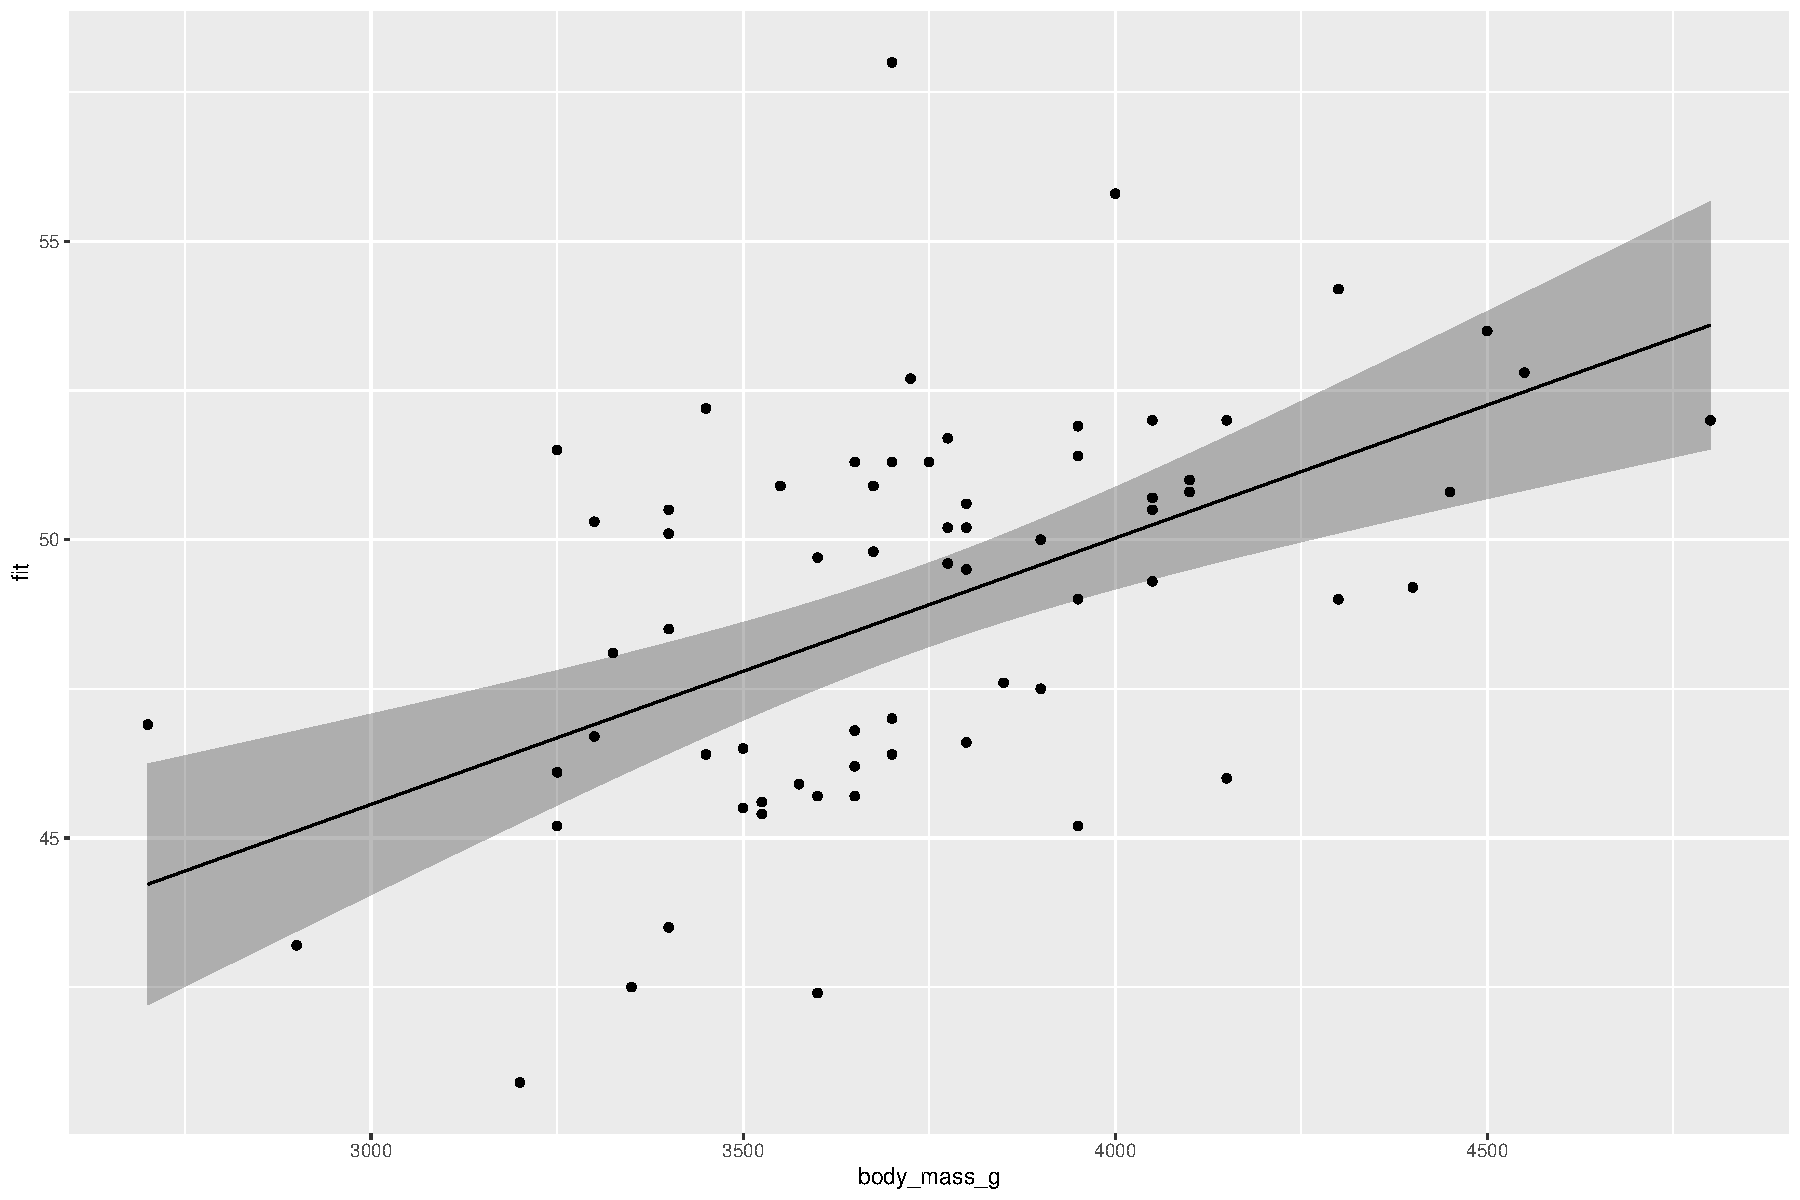
\includegraphics{Bayes_Lab_1_files/figure-pdf/unnamed-chunk-16-1.pdf}

If we wanted to, we could look at the residuals with help from the
\texttt{residuals()} function.

\begin{Shaded}
\begin{Highlighting}[]
\FunctionTok{residuals}\NormalTok{(fit1.ols)}
\end{Highlighting}
\end{Shaded}

\begin{verbatim}
         1          2          3          4          5          6          7 
-1.2936220  0.4213003  2.8369738 -2.5051894  3.9022718 -4.6018344 -0.5779485 
         8          9         10         11         12         13         14 
 2.3907044 -4.6943732  2.6138391 -2.5324303  2.6791371 -1.6861609  1.7518962 
        15         16         17         18         19         20         21 
-2.2283241  0.2518962  3.3989168  9.3138391 -1.1704873 -2.6100467 -5.8398915 
        22         23         24         25         26         27         28 
 1.1526474 -1.9160056  1.4675697 -0.2010832  1.3056268  3.1526474  0.3675697 
        29         30         31         32         33         34         35 
-2.2861609  0.3205492 -5.5548138  2.8362227 -4.6242179  0.5287615  1.4601085 
        36         37         38         39         40         41         42 
-2.0786997 -1.7555650 -1.5951243  2.6765332  1.2436839 -0.8018344 -2.2630262 
        43         44         45         46         47         48         49 
 2.8832432 -2.2936220  2.3254065 -1.2331814  2.7526474 -2.3637773  4.8220515 
        50         51         52         53         54         55         56 
 1.2254065  1.0873494  1.5981656 -2.5398915  0.4518962 -4.6242179  4.6295127 
        57         58         59         60         61         62         63 
-1.4779485 -0.9481038  1.0675697 -2.3051894  2.0981656 -1.6630262 -2.7630262 
        64         65         66         67         68 
 5.7750309 -3.8473526  0.5791371  0.3287615  1.1791371 
\end{verbatim}

Here we might put them in a tibble and display them in a plot.

\begin{Shaded}
\begin{Highlighting}[]
\CommentTok{\# put them in a tibble}
\FunctionTok{tibble}\NormalTok{(}\AttributeTok{r =} \FunctionTok{residuals}\NormalTok{(fit1.ols)) }\SpecialCharTok{\%\textgreater{}\%} 
  \CommentTok{\# plot!}
  \FunctionTok{ggplot}\NormalTok{(}\FunctionTok{aes}\NormalTok{(}\AttributeTok{x =}\NormalTok{ r)) }\SpecialCharTok{+}
  \FunctionTok{geom\_histogram}\NormalTok{(}\AttributeTok{binwidth =} \DecValTok{1}\NormalTok{)}
\end{Highlighting}
\end{Shaded}

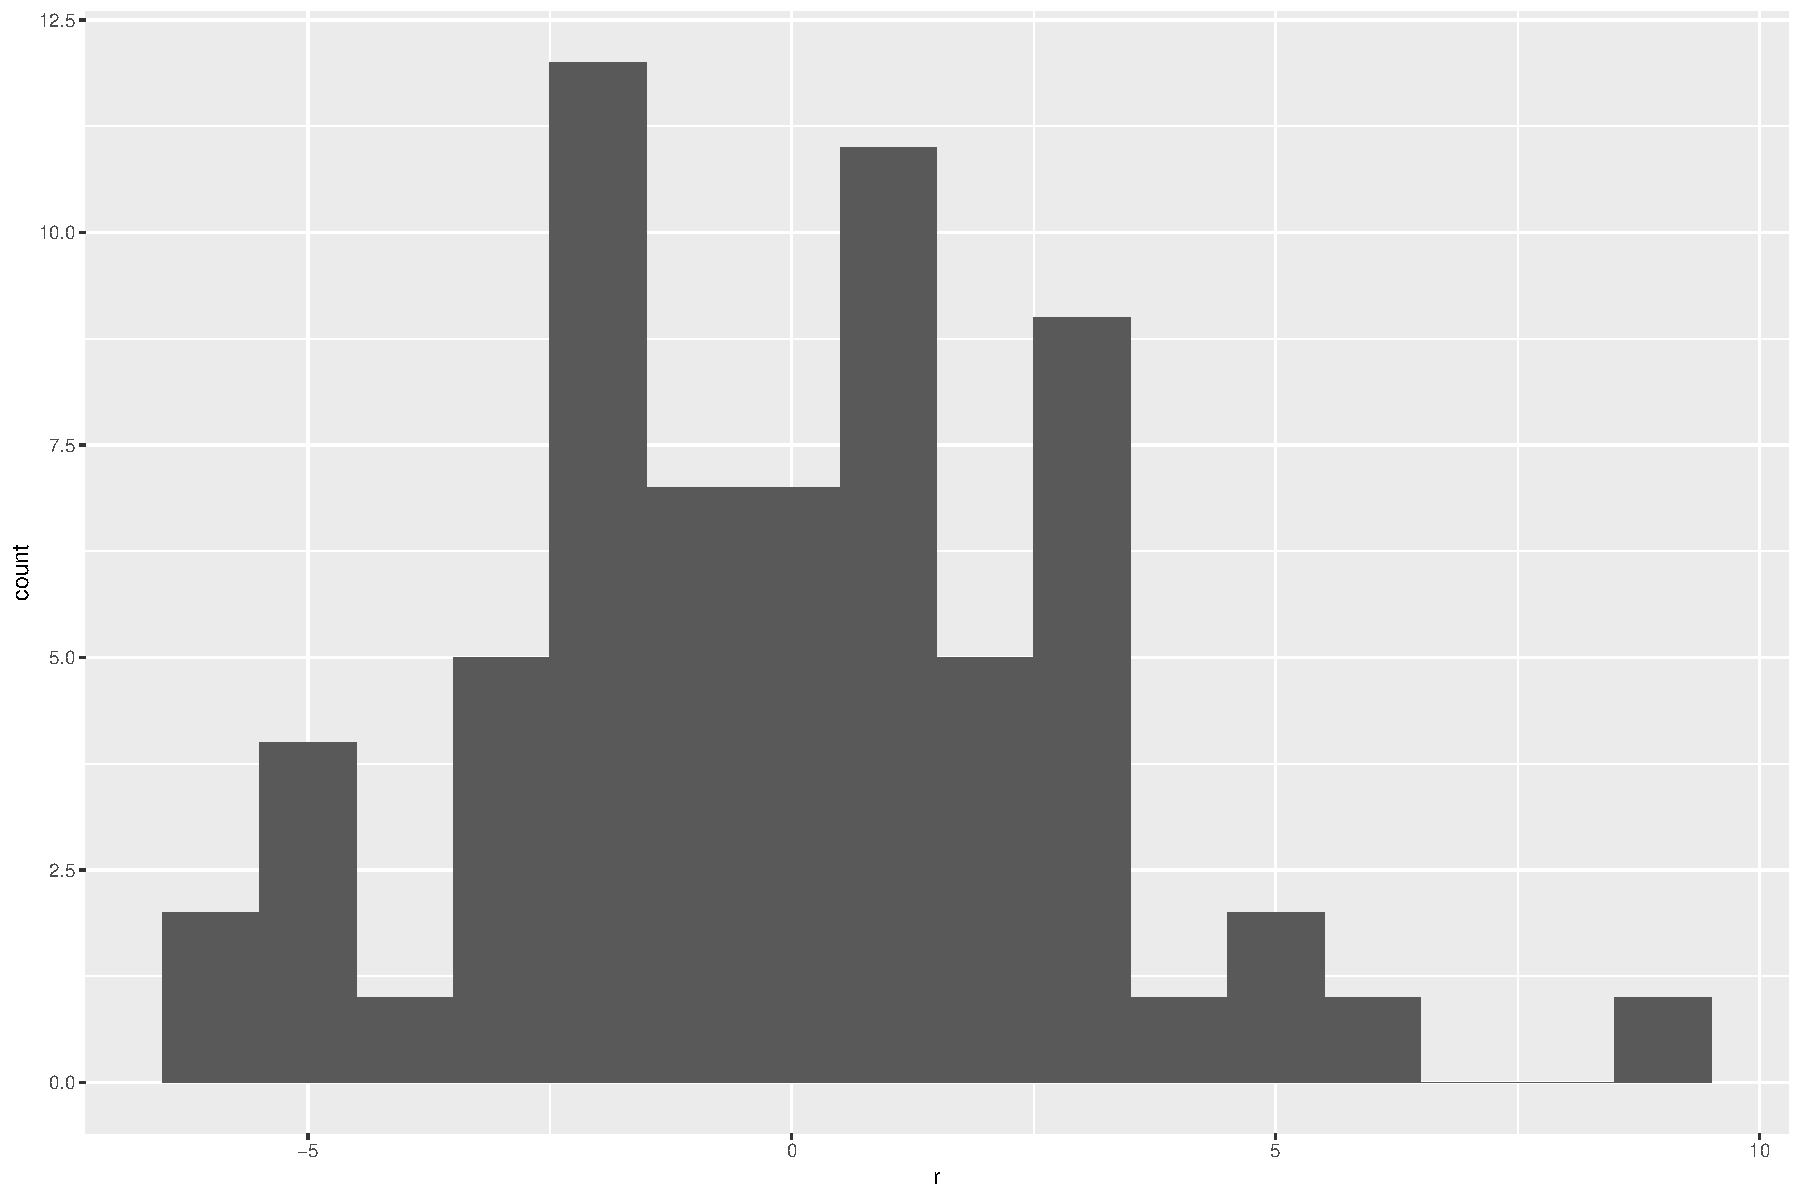
\includegraphics{Bayes_Lab_1_files/figure-pdf/unnamed-chunk-18-1.pdf}

\subsubsection{Question 1.2: Can you predict what the mean value, and
standard deviations will be? Why? Calculate it. Compare this against
outputs in summary(fit1.ols) and explain. Map the values you find to the
latex equations
before.}\label{question-1.2-can-you-predict-what-the-mean-value-and-standard-deviations-will-be-why-calculate-it.-compare-this-against-outputs-in-summaryfit1.ols-and-explain.-map-the-values-you-find-to-the-latex-equations-before.}

\begin{Shaded}
\begin{Highlighting}[]
\CommentTok{\# Slope}
\NormalTok{slope }\OtherTok{=} \FunctionTok{cov}\NormalTok{(chinstrap}\SpecialCharTok{$}\NormalTok{body\_mass\_g, chinstrap}\SpecialCharTok{$}\NormalTok{bill\_length\_mm) }\SpecialCharTok{/} \FunctionTok{var}\NormalTok{(chinstrap}\SpecialCharTok{$}\NormalTok{body\_mass\_g)}
\NormalTok{slope}
\end{Highlighting}
\end{Shaded}

\begin{verbatim}
[1] 0.004462694
\end{verbatim}

\begin{Shaded}
\begin{Highlighting}[]
\NormalTok{res }\OtherTok{=} \FunctionTok{residuals}\NormalTok{(fit1.ols)}
\NormalTok{var\_res }\OtherTok{=} \FunctionTok{sum}\NormalTok{(res}\SpecialCharTok{\^{}}\DecValTok{2}\NormalTok{) }\SpecialCharTok{/}\NormalTok{ (}\FunctionTok{length}\NormalTok{(chinstrap) }\SpecialCharTok{{-}} \DecValTok{2}\NormalTok{)}
\NormalTok{var\_res }\SpecialCharTok{/} \FunctionTok{sum}\NormalTok{((chinstrap}\SpecialCharTok{$}\NormalTok{body\_mass\_g }\SpecialCharTok{{-}} \FunctionTok{mean}\NormalTok{(chinstrap}\SpecialCharTok{$}\NormalTok{body\_mass\_g))}\SpecialCharTok{\^{}}\DecValTok{2}\NormalTok{)}
\end{Highlighting}
\end{Shaded}

\begin{verbatim}
[1] 9.262102e-06
\end{verbatim}

\begin{Shaded}
\begin{Highlighting}[]
\CommentTok{\# Intercept}
\FunctionTok{mean}\NormalTok{(chinstrap}\SpecialCharTok{$}\NormalTok{bill\_length\_mm) }\SpecialCharTok{{-}}\NormalTok{ slope }\SpecialCharTok{*} \FunctionTok{mean}\NormalTok{(chinstrap}\SpecialCharTok{$}\NormalTok{body\_mass\_g)}
\end{Highlighting}
\end{Shaded}

\begin{verbatim}
[1] 32.17419
\end{verbatim}

\begin{Shaded}
\begin{Highlighting}[]
\FunctionTok{sd}\NormalTok{(chinstrap}\SpecialCharTok{$}\NormalTok{bill\_length\_mm)}
\end{Highlighting}
\end{Shaded}

\begin{verbatim}
[1] 3.339256
\end{verbatim}

\begin{verbatim}
The estimate for the intercept is 32.17 with a standard deviation of 3.40. The standard deviation is not computed from the residuals but the simple SD of the y is a good enough estimate here. Both are pretty close to the estimated value from the model.

The mean value for the slope is 0.0045 and the standard deviation is 9.26e-06. These are quite similar to the values from our ols model.
\end{verbatim}

\[
\begin{align}
\text{bill_length_mm}_i = 32.17 + 0.0045 * \text{body_mass_g}_i
\end{align}
\]

\subsection{Bayes with default
settings}\label{bayes-with-default-settings}

We'll be fitting our Bayesian models with the \textbf{brms} package. The
primary function is \texttt{brm()}.

\texttt{brm()} can work a lot like the OLS-based \texttt{lm()} function.
For example, here's how to fit a Bayesian version of our OLS model
\texttt{fit1.ols}.

\begin{Shaded}
\begin{Highlighting}[]
\NormalTok{fit1.b }\OtherTok{\textless{}{-}} \FunctionTok{brm}\NormalTok{(}
  \AttributeTok{data =}\NormalTok{ chinstrap,}
\NormalTok{  bill\_length\_mm }\SpecialCharTok{\textasciitilde{}} \DecValTok{1} \SpecialCharTok{+}\NormalTok{ body\_mass\_g}
\NormalTok{)}
\end{Highlighting}
\end{Shaded}

Notice what's happening in the console, below. We'll get into the
details of what just happened later. For now, appreciate we just fit our
first Bayesian model, and it wasn't all that hard.

Summarize the model.

\begin{Shaded}
\begin{Highlighting}[]
\FunctionTok{summary}\NormalTok{(fit1.b)}
\end{Highlighting}
\end{Shaded}

\begin{verbatim}
 Family: gaussian 
  Links: mu = identity; sigma = identity 
Formula: bill_length_mm ~ 1 + body_mass_g 
   Data: chinstrap (Number of observations: 68) 
  Draws: 4 chains, each with iter = 2000; warmup = 1000; thin = 1;
         total post-warmup draws = 4000

Regression Coefficients:
            Estimate Est.Error l-95% CI u-95% CI Rhat Bulk_ESS Tail_ESS
Intercept      32.14      3.50    25.45    38.89 1.00     4820     2982
body_mass_g     0.00      0.00     0.00     0.01 1.00     4861     3170

Further Distributional Parameters:
      Estimate Est.Error l-95% CI u-95% CI Rhat Bulk_ESS Tail_ESS
sigma     2.92      0.26     2.48     3.50 1.00     2015     1688

Draws were sampled using sampling(NUTS). For each parameter, Bulk_ESS
and Tail_ESS are effective sample size measures, and Rhat is the potential
scale reduction factor on split chains (at convergence, Rhat = 1).
\end{verbatim}

\subsubsection{\texorpdfstring{Question 1.3: Contrast the language of in
the \texttt{brm()} output from the in the \texttt{lm()} output. Ignore
`Rhat,' `Bulk\_ESS,' and `Tail\_ESS' for
now.}{Question 1.3: Contrast the language of in the brm() output from the in the lm() output. Ignore `Rhat,' `Bulk\_ESS,' and `Tail\_ESS' for now.}}\label{question-1.3-contrast-the-language-of-in-the-brm-output-from-the-in-the-lm-output.-ignore-rhat-bulk_ess-and-tail_ess-for-now.}

\begin{verbatim}
The estimated values are pretty similar in both models. 

The frequentist model shows t and p value for all parameters.

The bayesian model shows the 95% confidence interval for all parameters.
\end{verbatim}

We can get a quick and dirty plot of the fitted line with the
\texttt{conditional\_effects()} function.

\begin{Shaded}
\begin{Highlighting}[]
\FunctionTok{conditional\_effects}\NormalTok{(fit1.b)}
\end{Highlighting}
\end{Shaded}

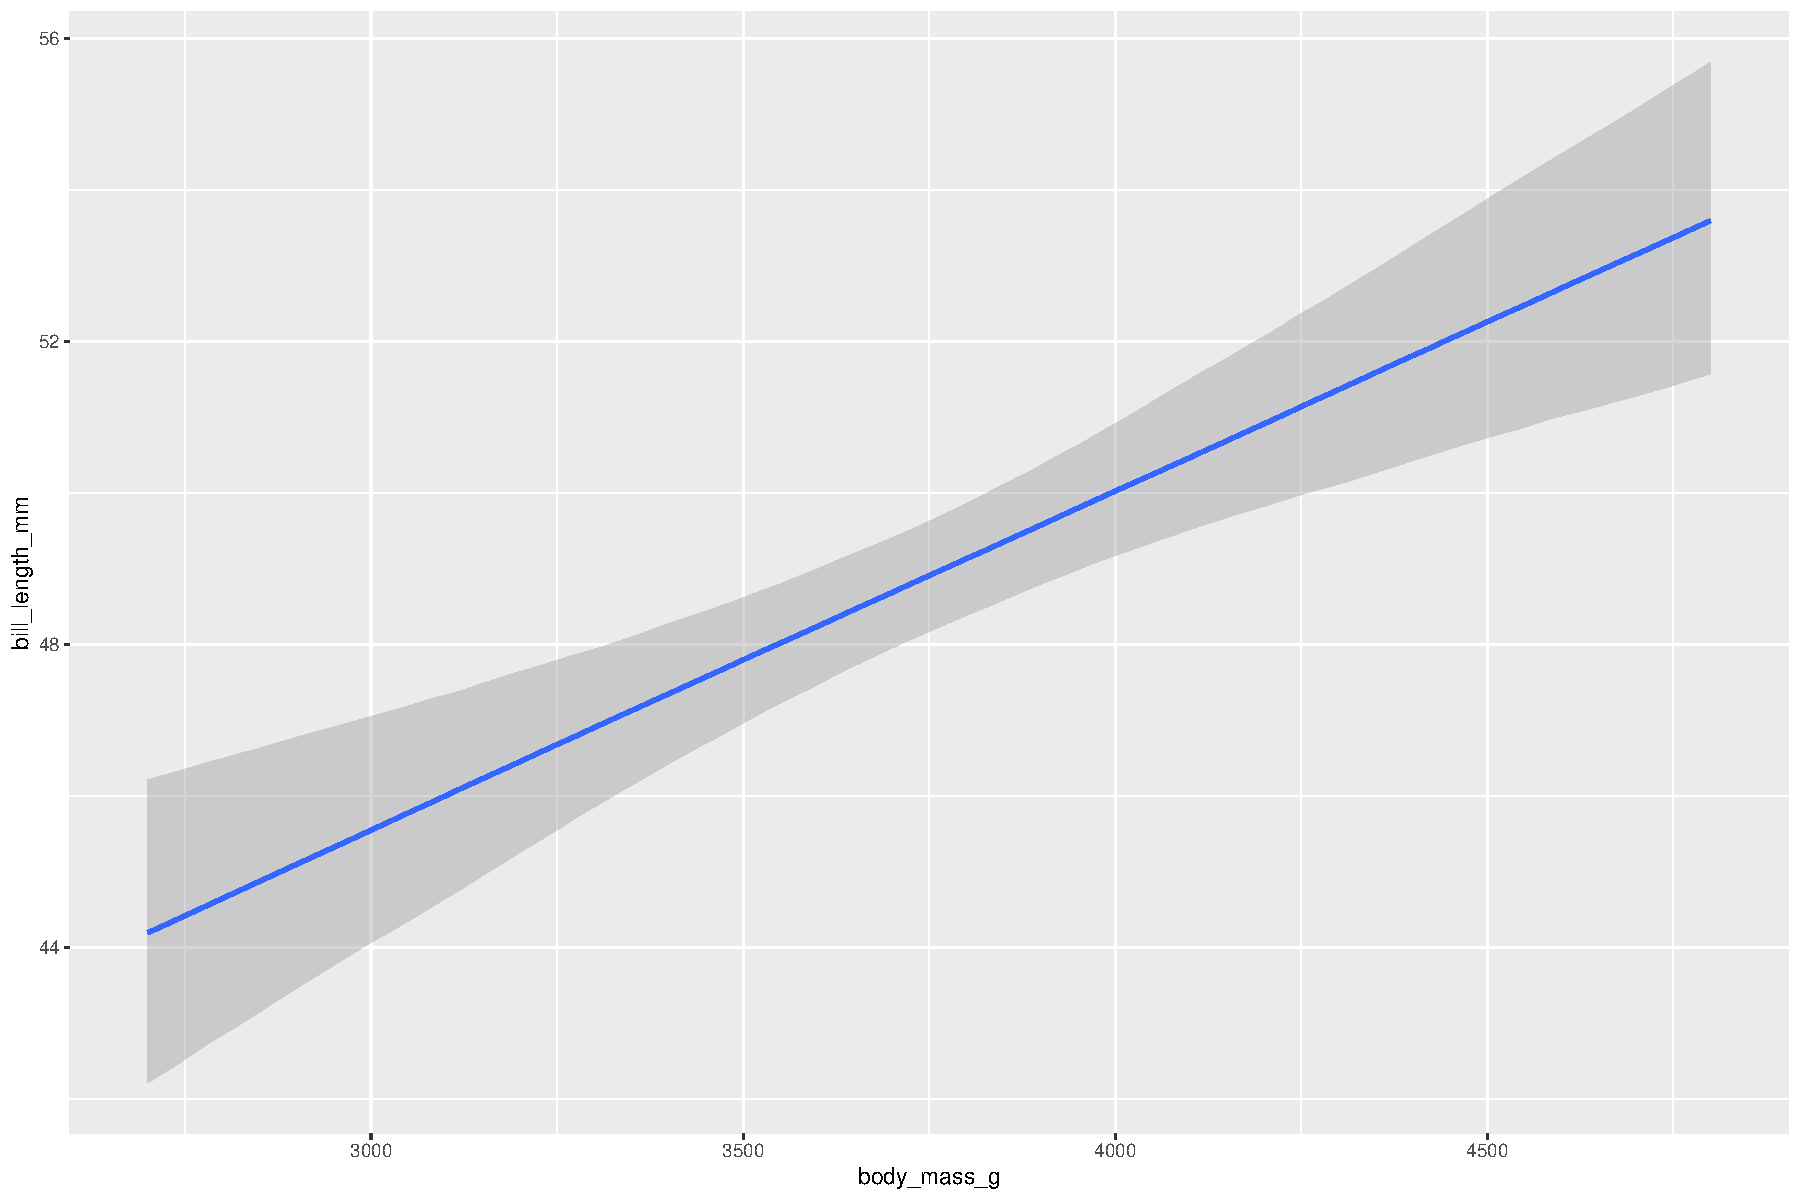
\includegraphics{Bayes_Lab_1_files/figure-pdf/unnamed-chunk-21-1.pdf}

\begin{Shaded}
\begin{Highlighting}[]
\CommentTok{\# \%\textgreater{}\% }
\CommentTok{\#   plot(points = TRUE)}
\end{Highlighting}
\end{Shaded}

\subsection{Coefficients and coefficient
plots}\label{coefficients-and-coefficient-plots}

We might want to compare the coefficient summaries from the OLS model to
those from the Bayesian model. Here's the frequentist summary:

\begin{Shaded}
\begin{Highlighting}[]
\FunctionTok{cbind}\NormalTok{(}\FunctionTok{coef}\NormalTok{(fit1.ols),              }\CommentTok{\# point estimates}
      \FunctionTok{sqrt}\NormalTok{(}\FunctionTok{diag}\NormalTok{(}\FunctionTok{vcov}\NormalTok{(fit1.ols))),  }\CommentTok{\# standard errors}
      \FunctionTok{confint}\NormalTok{(fit1.ols))           }\CommentTok{\# 95\% CIs}
\end{Highlighting}
\end{Shaded}

\begin{verbatim}
                                             2.5 %       97.5 %
(Intercept) 32.174192865 3.4433622902 25.299298235 39.049087495
body_mass_g  0.004462694 0.0009176106  0.002630625  0.006294763
\end{verbatim}

We can compute a focused summary of the Bayesian model with the
\texttt{fixef()} function.

\begin{Shaded}
\begin{Highlighting}[]
\FunctionTok{fixef}\NormalTok{(fit1.b)}
\end{Highlighting}
\end{Shaded}

\begin{verbatim}
                Estimate    Est.Error         Q2.5        Q97.5
Intercept   32.139661018 3.4974943137 25.449370922 38.886468789
body_mass_g  0.004471587 0.0009315803  0.002675154  0.006246179
\end{verbatim}

In this case, the results are very similar.

We can also pull this information from our OLS model with the
\texttt{broom::tidy()} function.

\begin{Shaded}
\begin{Highlighting}[]
\FunctionTok{tidy}\NormalTok{(fit1.ols, }\AttributeTok{conf.int =} \ConstantTok{TRUE}\NormalTok{)}
\end{Highlighting}
\end{Shaded}

\begin{verbatim}
# A tibble: 2 x 7
  term        estimate std.error statistic  p.value conf.low conf.high
  <chr>          <dbl>     <dbl>     <dbl>    <dbl>    <dbl>     <dbl>
1 (Intercept) 32.2      3.44          9.34 1.07e-13 25.3      39.0    
2 body_mass_g  0.00446  0.000918      4.86 7.48e- 6  0.00263   0.00629
\end{verbatim}

If you would like to use the \texttt{tidy()} function with your
\textbf{brms} models, it will have to be the version of \texttt{tidy()}
from the \textbf{broom.mixed} package.

\begin{Shaded}
\begin{Highlighting}[]
\FunctionTok{tidy}\NormalTok{(fit1.b)}
\end{Highlighting}
\end{Shaded}

\begin{verbatim}
# A tibble: 3 x 8
  effect   component group    term         estimate std.error conf.low conf.high
  <chr>    <chr>     <chr>    <chr>           <dbl>     <dbl>    <dbl>     <dbl>
1 fixed    cond      <NA>     (Intercept)  32.1      3.50     25.4      38.9    
2 fixed    cond      <NA>     body_mass_g   0.00447  0.000932  0.00268   0.00625
3 ran_pars cond      Residual sd__Observa~  2.92     0.258     2.48      3.50   
\end{verbatim}

Here's how to wrangle and combine these two results into a single data
frame. Then we'll make a coefficient plot.

\begin{Shaded}
\begin{Highlighting}[]
\FunctionTok{bind\_rows}\NormalTok{(}
  \FunctionTok{tidy}\NormalTok{(fit1.ols, }\AttributeTok{conf.int =} \ConstantTok{TRUE}\NormalTok{) }\SpecialCharTok{\%\textgreater{}\%} \FunctionTok{select}\NormalTok{(term, estimate, }\FunctionTok{contains}\NormalTok{(}\StringTok{"conf"}\NormalTok{)),}
  \FunctionTok{tidy}\NormalTok{(fit1.b) }\SpecialCharTok{\%\textgreater{}\%} \FunctionTok{select}\NormalTok{(term, estimate, }\FunctionTok{contains}\NormalTok{(}\StringTok{"conf"}\NormalTok{)) }\SpecialCharTok{\%\textgreater{}\%} \FunctionTok{filter}\NormalTok{(term }\SpecialCharTok{!=} \StringTok{"sd\_\_Observation"}\NormalTok{)}
\NormalTok{) }\SpecialCharTok{\%\textgreater{}\%} 
  \FunctionTok{mutate}\NormalTok{(}\AttributeTok{method =} \FunctionTok{rep}\NormalTok{(}\FunctionTok{c}\NormalTok{(}\StringTok{"lm()"}\NormalTok{, }\StringTok{"brm()"}\NormalTok{), }\AttributeTok{each =} \DecValTok{2}\NormalTok{)) }\SpecialCharTok{\%\textgreater{}\%} 
  
  \FunctionTok{ggplot}\NormalTok{(}\FunctionTok{aes}\NormalTok{(}\AttributeTok{x =}\NormalTok{ estimate, }\AttributeTok{xmin =}\NormalTok{ conf.low, }\AttributeTok{xmax =}\NormalTok{ conf.high, }\AttributeTok{y =}\NormalTok{ method)) }\SpecialCharTok{+}
  \FunctionTok{geom\_pointrange}\NormalTok{() }\SpecialCharTok{+}
  \FunctionTok{scale\_x\_continuous}\NormalTok{(}\StringTok{"parameter space"}\NormalTok{, }\AttributeTok{expand =} \FunctionTok{expansion}\NormalTok{(}\AttributeTok{mult =} \FloatTok{0.2}\NormalTok{)) }\SpecialCharTok{+}
  \FunctionTok{scale\_y\_discrete}\NormalTok{(}\AttributeTok{expand =} \FunctionTok{expansion}\NormalTok{(}\AttributeTok{mult =} \DecValTok{5}\NormalTok{)) }\SpecialCharTok{+}
  \FunctionTok{facet\_wrap}\NormalTok{(}\SpecialCharTok{\textasciitilde{}}\NormalTok{ term, }\AttributeTok{scales =} \StringTok{"free\_x"}\NormalTok{)}
\end{Highlighting}
\end{Shaded}

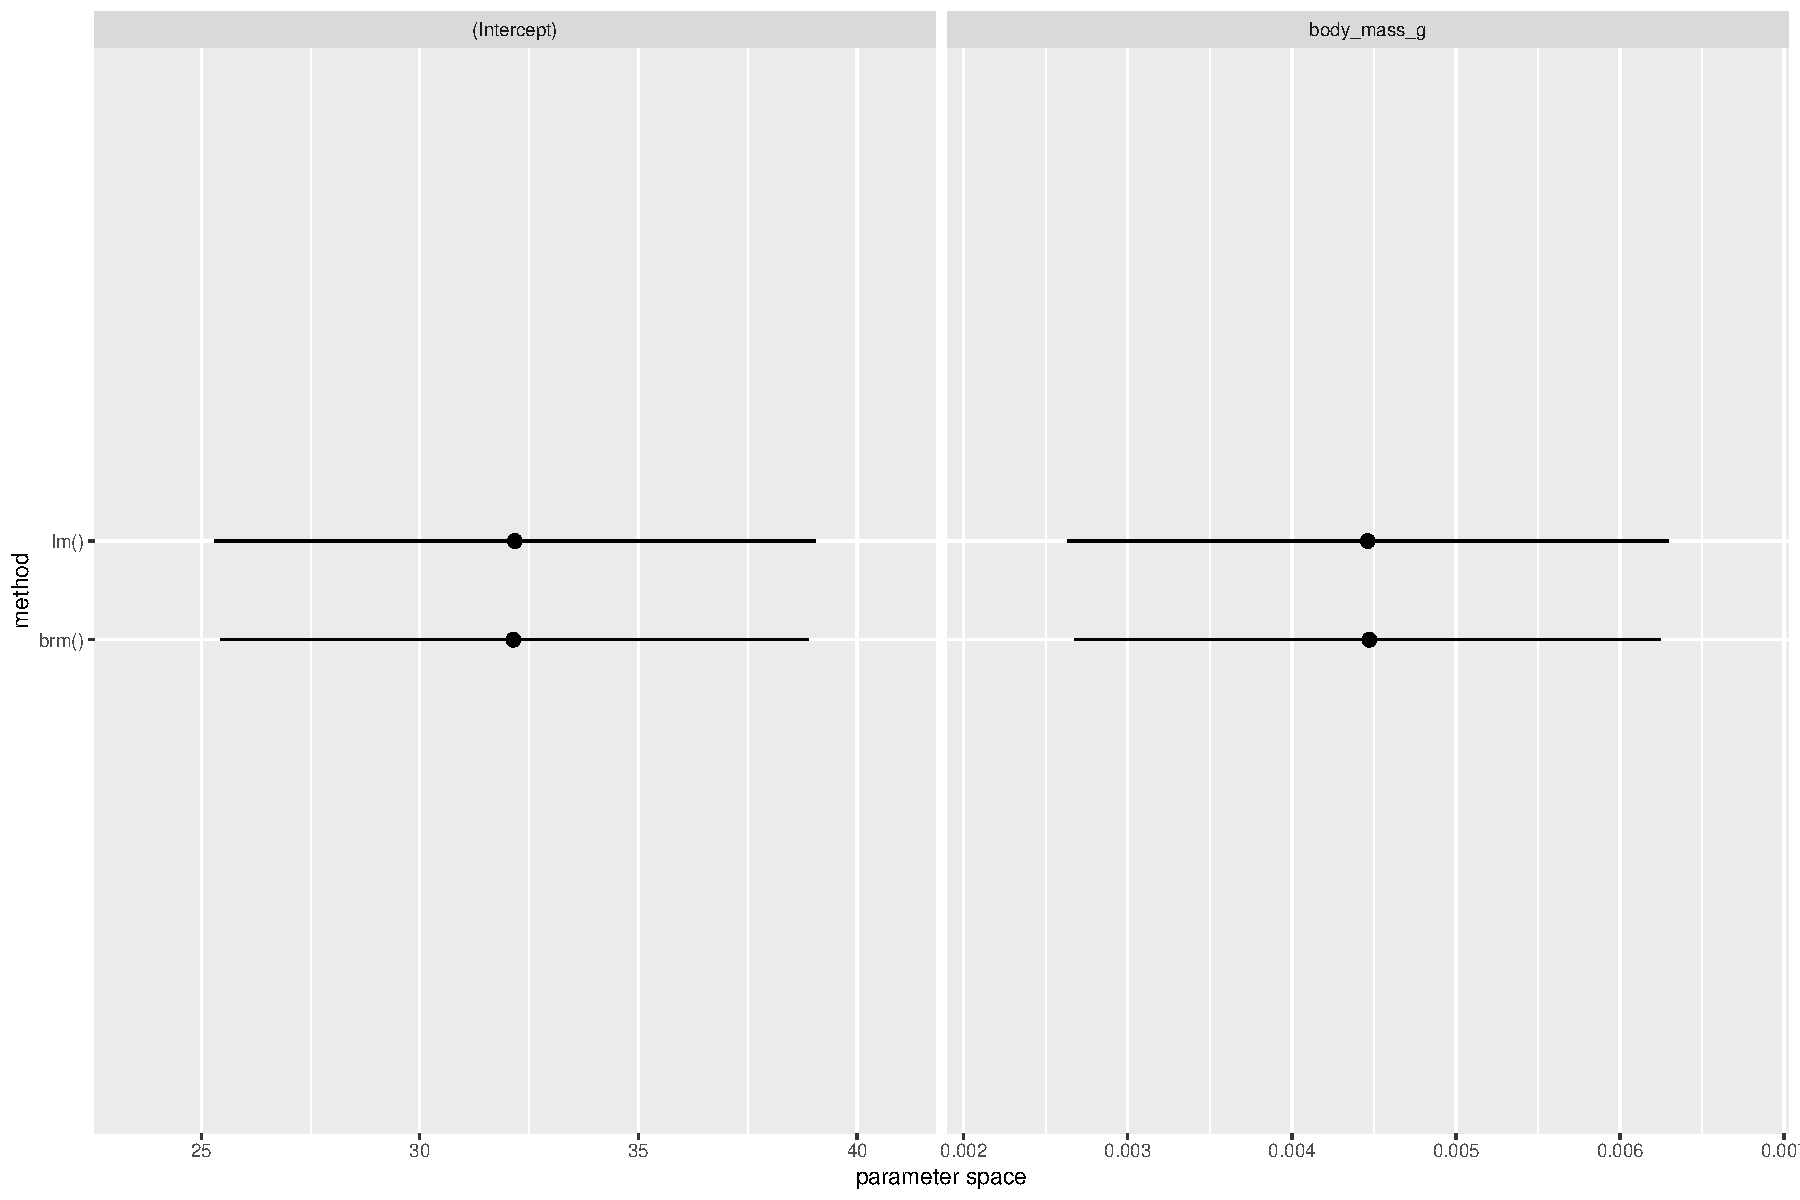
\includegraphics{Bayes_Lab_1_files/figure-pdf/unnamed-chunk-26-1.pdf}

At a superficial level for simple conventional regression type models,
the results from a Bayesian \texttt{brm()} model will be very similar to
those from an OLS \texttt{lm()} model. This will not always be case, and
even in this example there are many differences once we look below the
surface.

\subsection{More Questions/Exercise}\label{more-questionsexercise}

Go back to the full \texttt{penguins} data set. This time, make a subset
of the data called \texttt{gentoo}, which is only the cases for which
\texttt{species\ ==\ "Gentoo"}.

\begin{Shaded}
\begin{Highlighting}[]
\NormalTok{gentoo }\OtherTok{\textless{}{-}}\NormalTok{ penguins }\SpecialCharTok{\%\textgreater{}\%} 
  \FunctionTok{filter}\NormalTok{(species }\SpecialCharTok{==} \StringTok{"Gentoo"}\NormalTok{)}
\end{Highlighting}
\end{Shaded}

Can you fit the same OLS model to these data?

\begin{Shaded}
\begin{Highlighting}[]
\NormalTok{fit2.ols }\OtherTok{\textless{}{-}} \FunctionTok{lm}\NormalTok{(}
  \AttributeTok{data =}\NormalTok{ gentoo,}
\NormalTok{  bill\_length\_mm }\SpecialCharTok{\textasciitilde{}} \DecValTok{1} \SpecialCharTok{+}\NormalTok{ body\_mass\_g}
\NormalTok{)}
\end{Highlighting}
\end{Shaded}

How about plotting the results with \texttt{predict()}?

\begin{Shaded}
\begin{Highlighting}[]
\NormalTok{gentoo\_filtered }\OtherTok{=}\NormalTok{ gentoo }\SpecialCharTok{\%\textgreater{}\%} \FunctionTok{filter}\NormalTok{(}\SpecialCharTok{!}\FunctionTok{is.na}\NormalTok{(body\_mass\_g))}
\NormalTok{od2 }\OtherTok{\textless{}{-}} \FunctionTok{tibble}\NormalTok{(}\AttributeTok{body\_mass\_g =}\NormalTok{ gentoo\_filtered}\SpecialCharTok{$}\NormalTok{body\_mass\_g)}
\FunctionTok{predict}\NormalTok{(fit2.ols,}
        \AttributeTok{interval =} \StringTok{"confidence"}\NormalTok{) }\SpecialCharTok{\%\textgreater{}\%} 
  \FunctionTok{data.frame}\NormalTok{() }\SpecialCharTok{\%\textgreater{}\%} 
  \FunctionTok{bind\_cols}\NormalTok{(od2) }\SpecialCharTok{\%\textgreater{}\%} 
  \FunctionTok{ggplot}\NormalTok{(}\FunctionTok{aes}\NormalTok{(}\AttributeTok{x =}\NormalTok{ body\_mass\_g)) }\SpecialCharTok{+}
  \CommentTok{\# 95\% confidence interval ribbon}
  \FunctionTok{geom\_ribbon}\NormalTok{(}\FunctionTok{aes}\NormalTok{(}\AttributeTok{ymin =}\NormalTok{ lwr, }\AttributeTok{ymax =}\NormalTok{ upr),}
              \AttributeTok{alpha =} \DecValTok{1}\SpecialCharTok{/}\DecValTok{3}\NormalTok{) }\SpecialCharTok{+}
  \CommentTok{\# point estimate line}
  \FunctionTok{geom\_line}\NormalTok{(}\FunctionTok{aes}\NormalTok{(}\AttributeTok{y =}\NormalTok{ fit)) }\SpecialCharTok{+}
  \FunctionTok{geom\_point}\NormalTok{(}\AttributeTok{data =}\NormalTok{ gentoo\_filtered,}
             \FunctionTok{aes}\NormalTok{(}\AttributeTok{y =}\NormalTok{ bill\_length\_mm))}
\end{Highlighting}
\end{Shaded}

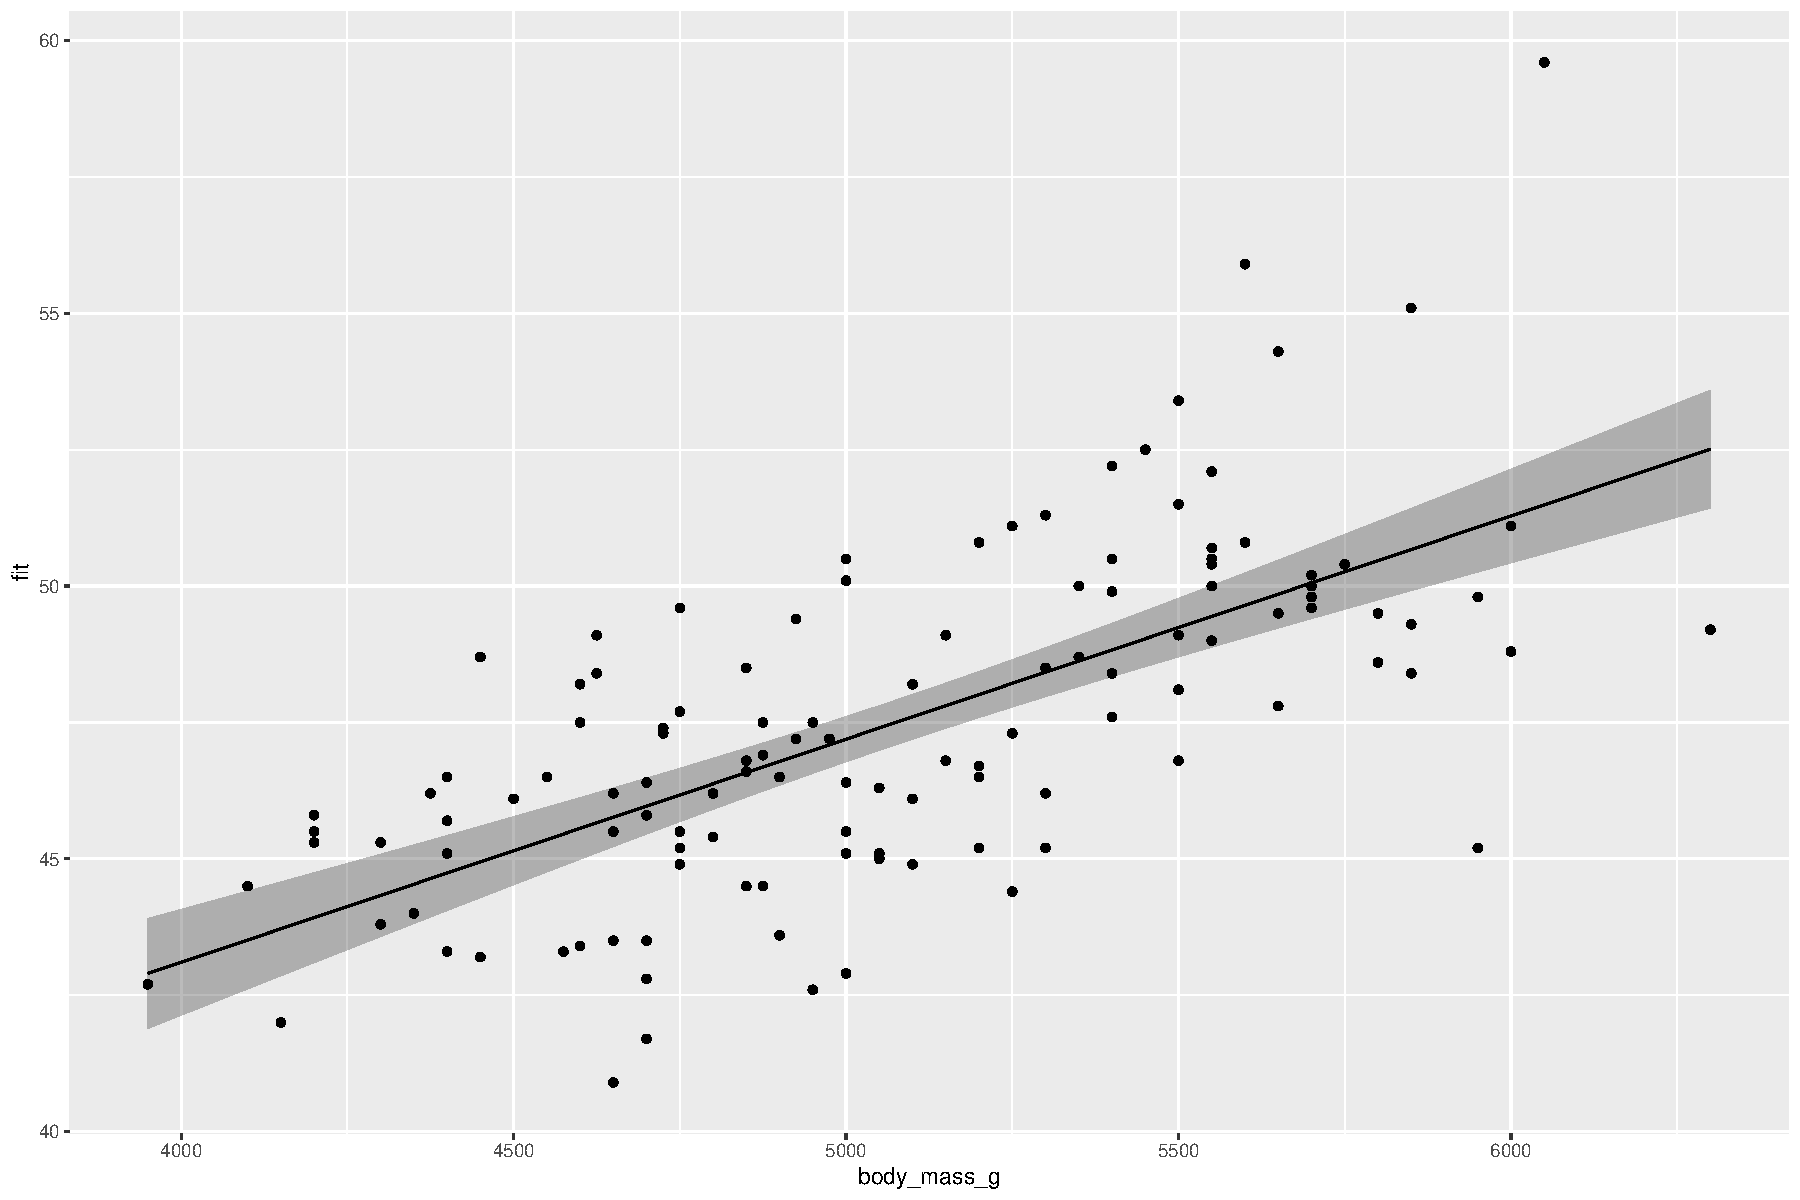
\includegraphics{Bayes_Lab_1_files/figure-pdf/unnamed-chunk-29-1.pdf}

\begin{Shaded}
\begin{Highlighting}[]
\NormalTok{nd2 }\OtherTok{\textless{}{-}} \FunctionTok{tibble}\NormalTok{(}\AttributeTok{body\_mass\_g =} \FunctionTok{seq}\NormalTok{(}\AttributeTok{from =} \FunctionTok{min}\NormalTok{(gentoo}\SpecialCharTok{$}\NormalTok{body\_mass\_g, }\AttributeTok{na.rm=}\ConstantTok{TRUE}\NormalTok{),}
                               \AttributeTok{to =} \FunctionTok{max}\NormalTok{(gentoo}\SpecialCharTok{$}\NormalTok{body\_mass\_g, }\AttributeTok{na.rm=}\ConstantTok{TRUE}\NormalTok{),}
                               \AttributeTok{length.out =} \DecValTok{50}\NormalTok{))}

\FunctionTok{predict}\NormalTok{(fit2.ols,}
        \AttributeTok{interval =} \StringTok{"confidence"}\NormalTok{,}
        \AttributeTok{newdata =}\NormalTok{ nd2) }\SpecialCharTok{\%\textgreater{}\%} 
  \FunctionTok{data.frame}\NormalTok{() }\SpecialCharTok{\%\textgreater{}\%} 
  \FunctionTok{bind\_cols}\NormalTok{(nd2) }\SpecialCharTok{\%\textgreater{}\%} 
  \FunctionTok{ggplot}\NormalTok{(}\FunctionTok{aes}\NormalTok{(}\AttributeTok{x =}\NormalTok{ body\_mass\_g)) }\SpecialCharTok{+}
  \CommentTok{\# 95\% confidence interval ribbon}
  \FunctionTok{geom\_ribbon}\NormalTok{(}\FunctionTok{aes}\NormalTok{(}\AttributeTok{ymin =}\NormalTok{ lwr, }\AttributeTok{ymax =}\NormalTok{ upr),}
              \AttributeTok{alpha =} \DecValTok{1}\SpecialCharTok{/}\DecValTok{3}\NormalTok{) }\SpecialCharTok{+}
  \CommentTok{\# point estimate line}
  \FunctionTok{geom\_line}\NormalTok{(}\FunctionTok{aes}\NormalTok{(}\AttributeTok{y =}\NormalTok{ fit)) }\SpecialCharTok{+}
  \FunctionTok{geom\_point}\NormalTok{(}\AttributeTok{data =}\NormalTok{ gentoo,}
             \FunctionTok{aes}\NormalTok{(}\AttributeTok{y =}\NormalTok{ bill\_length\_mm))}
\end{Highlighting}
\end{Shaded}

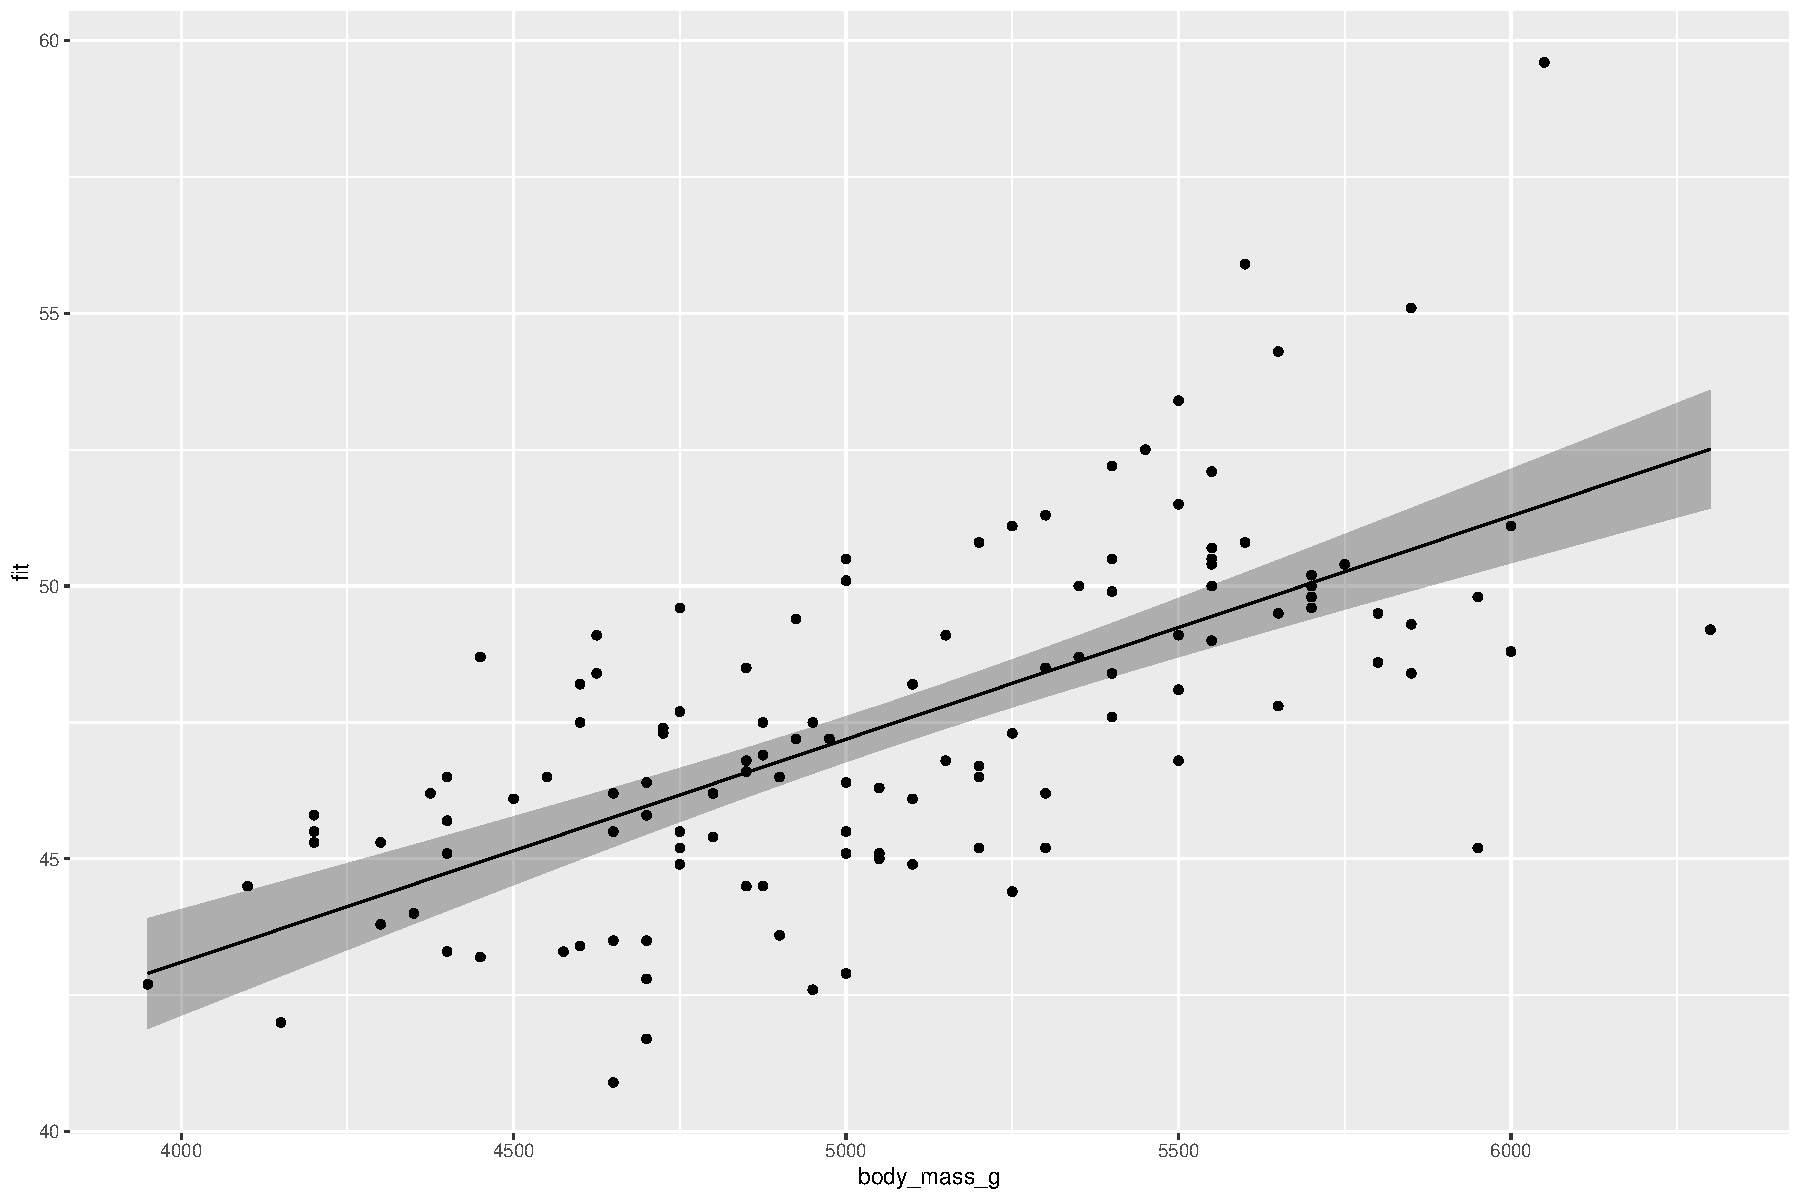
\includegraphics{Bayes_Lab_1_files/figure-pdf/unnamed-chunk-29-2.pdf}

Can you fit the same default Bayesian \texttt{brm()} model to these
data?

\begin{Shaded}
\begin{Highlighting}[]
\NormalTok{fit2.b }\OtherTok{\textless{}{-}} \FunctionTok{brm}\NormalTok{(}
  \AttributeTok{data =}\NormalTok{ gentoo,}
\NormalTok{  bill\_length\_mm }\SpecialCharTok{\textasciitilde{}} \DecValTok{1} \SpecialCharTok{+}\NormalTok{ body\_mass\_g}
\NormalTok{)}
\end{Highlighting}
\end{Shaded}

How about plotting the results with \texttt{conditional\_effects()}?

\begin{Shaded}
\begin{Highlighting}[]
\FunctionTok{conditional\_effects}\NormalTok{(fit2.b)}
\end{Highlighting}
\end{Shaded}

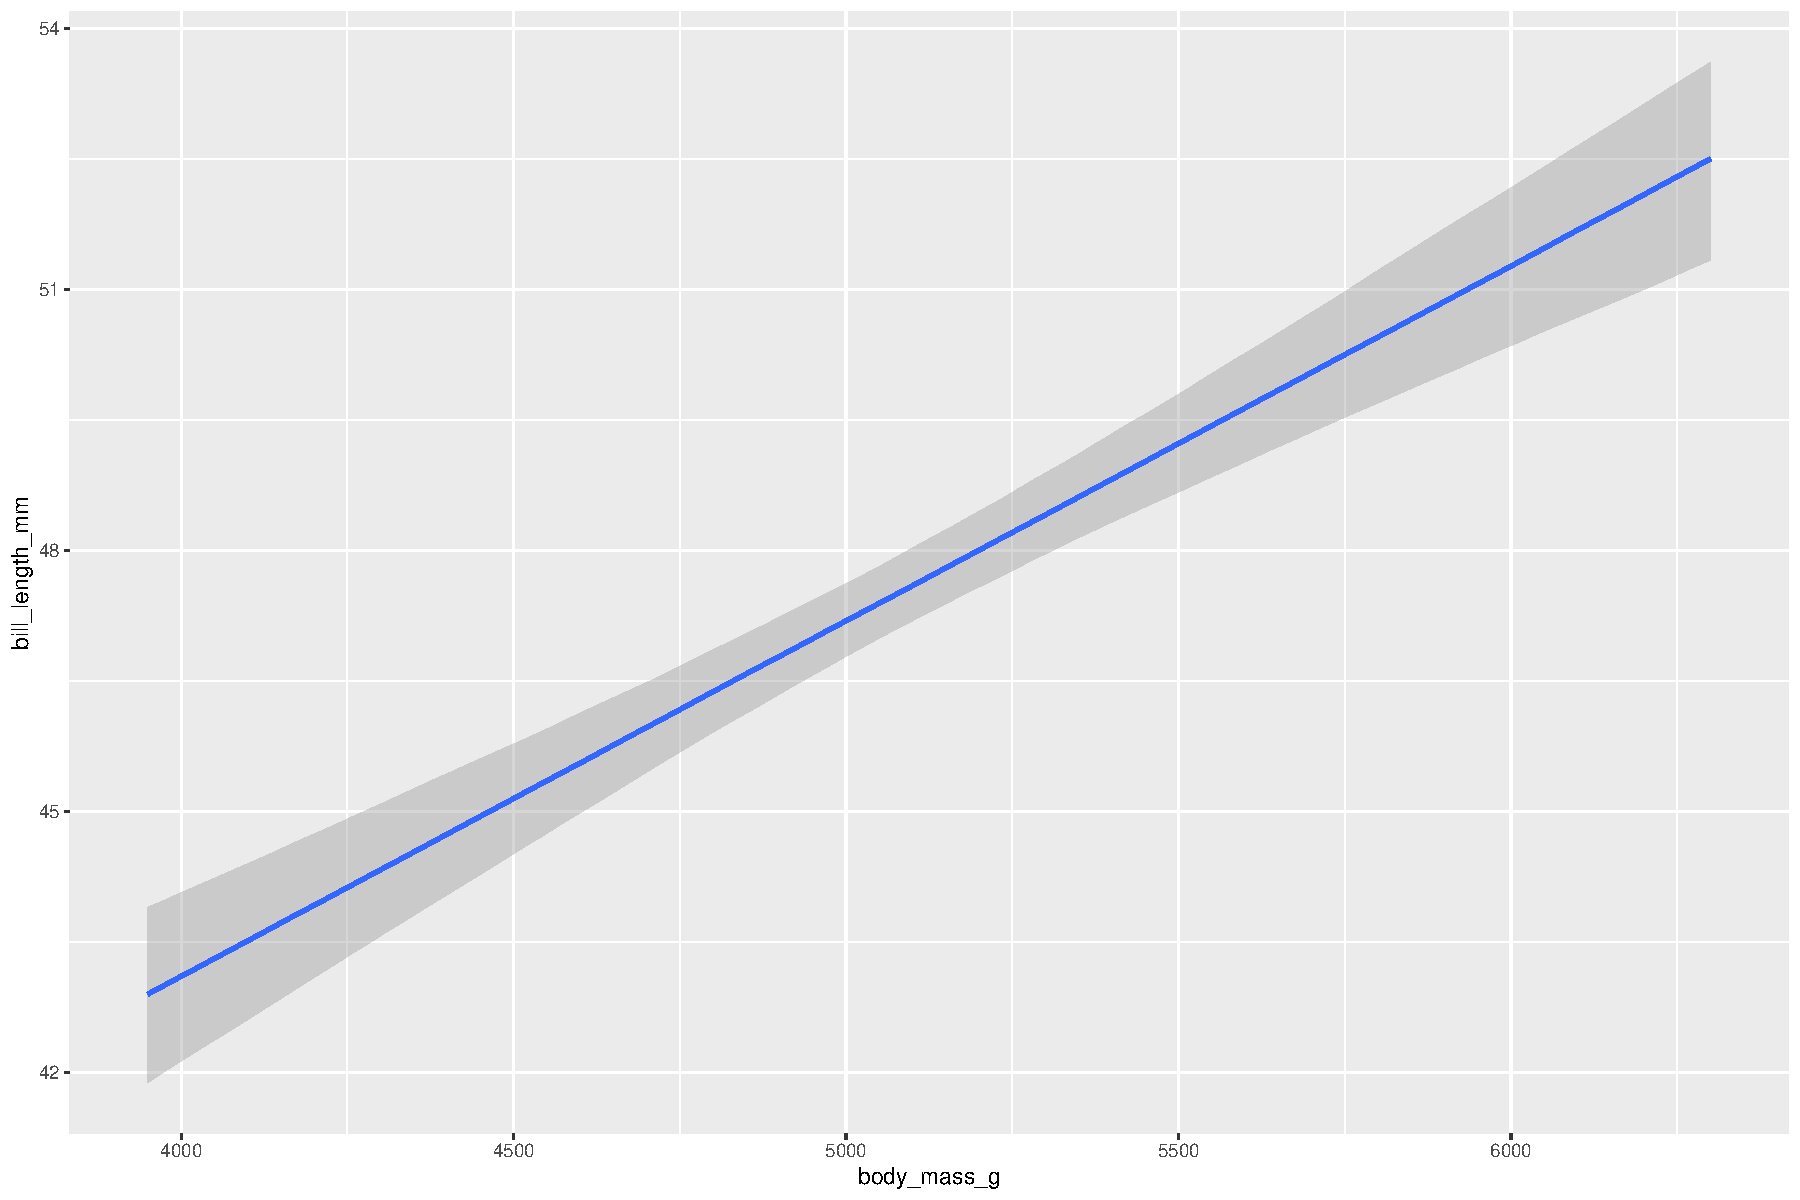
\includegraphics{Bayes_Lab_1_files/figure-pdf/unnamed-chunk-31-1.pdf}

\begin{Shaded}
\begin{Highlighting}[]
\CommentTok{\# \%\textgreater{}\% }
\CommentTok{\#   plot(points = TRUE)}
\end{Highlighting}
\end{Shaded}

Can you make a coefficient plot comparing the new OLS and Bayesian beta
coefficients?

\begin{Shaded}
\begin{Highlighting}[]
\FunctionTok{bind\_rows}\NormalTok{(}
  \FunctionTok{tidy}\NormalTok{(fit2.ols, }\AttributeTok{conf.int =} \ConstantTok{TRUE}\NormalTok{) }\SpecialCharTok{\%\textgreater{}\%} \FunctionTok{select}\NormalTok{(term, estimate, }\FunctionTok{contains}\NormalTok{(}\StringTok{"conf"}\NormalTok{)),}
  \FunctionTok{tidy}\NormalTok{(fit2.b) }\SpecialCharTok{\%\textgreater{}\%} \FunctionTok{select}\NormalTok{(term, estimate, }\FunctionTok{contains}\NormalTok{(}\StringTok{"conf"}\NormalTok{)) }\SpecialCharTok{\%\textgreater{}\%} \FunctionTok{filter}\NormalTok{(term }\SpecialCharTok{!=} \StringTok{"sd\_\_Observation"}\NormalTok{)}
\NormalTok{) }\SpecialCharTok{\%\textgreater{}\%} 
  \FunctionTok{mutate}\NormalTok{(}\AttributeTok{method =} \FunctionTok{rep}\NormalTok{(}\FunctionTok{c}\NormalTok{(}\StringTok{"lm()"}\NormalTok{, }\StringTok{"brm()"}\NormalTok{), }\AttributeTok{each =} \DecValTok{2}\NormalTok{)) }\SpecialCharTok{\%\textgreater{}\%} 
  
  \FunctionTok{ggplot}\NormalTok{(}\FunctionTok{aes}\NormalTok{(}\AttributeTok{x =}\NormalTok{ estimate, }\AttributeTok{xmin =}\NormalTok{ conf.low, }\AttributeTok{xmax =}\NormalTok{ conf.high, }\AttributeTok{y =}\NormalTok{ method)) }\SpecialCharTok{+}
  \FunctionTok{geom\_pointrange}\NormalTok{() }\SpecialCharTok{+}
  \FunctionTok{scale\_x\_continuous}\NormalTok{(}\StringTok{"parameter space"}\NormalTok{, }\AttributeTok{expand =} \FunctionTok{expansion}\NormalTok{(}\AttributeTok{mult =} \FloatTok{0.2}\NormalTok{)) }\SpecialCharTok{+}
  \FunctionTok{scale\_y\_discrete}\NormalTok{(}\AttributeTok{expand =} \FunctionTok{expansion}\NormalTok{(}\AttributeTok{mult =} \DecValTok{5}\NormalTok{)) }\SpecialCharTok{+}
  \FunctionTok{facet\_wrap}\NormalTok{(}\SpecialCharTok{\textasciitilde{}}\NormalTok{ term, }\AttributeTok{scales =} \StringTok{"free\_x"}\NormalTok{)}
\end{Highlighting}
\end{Shaded}

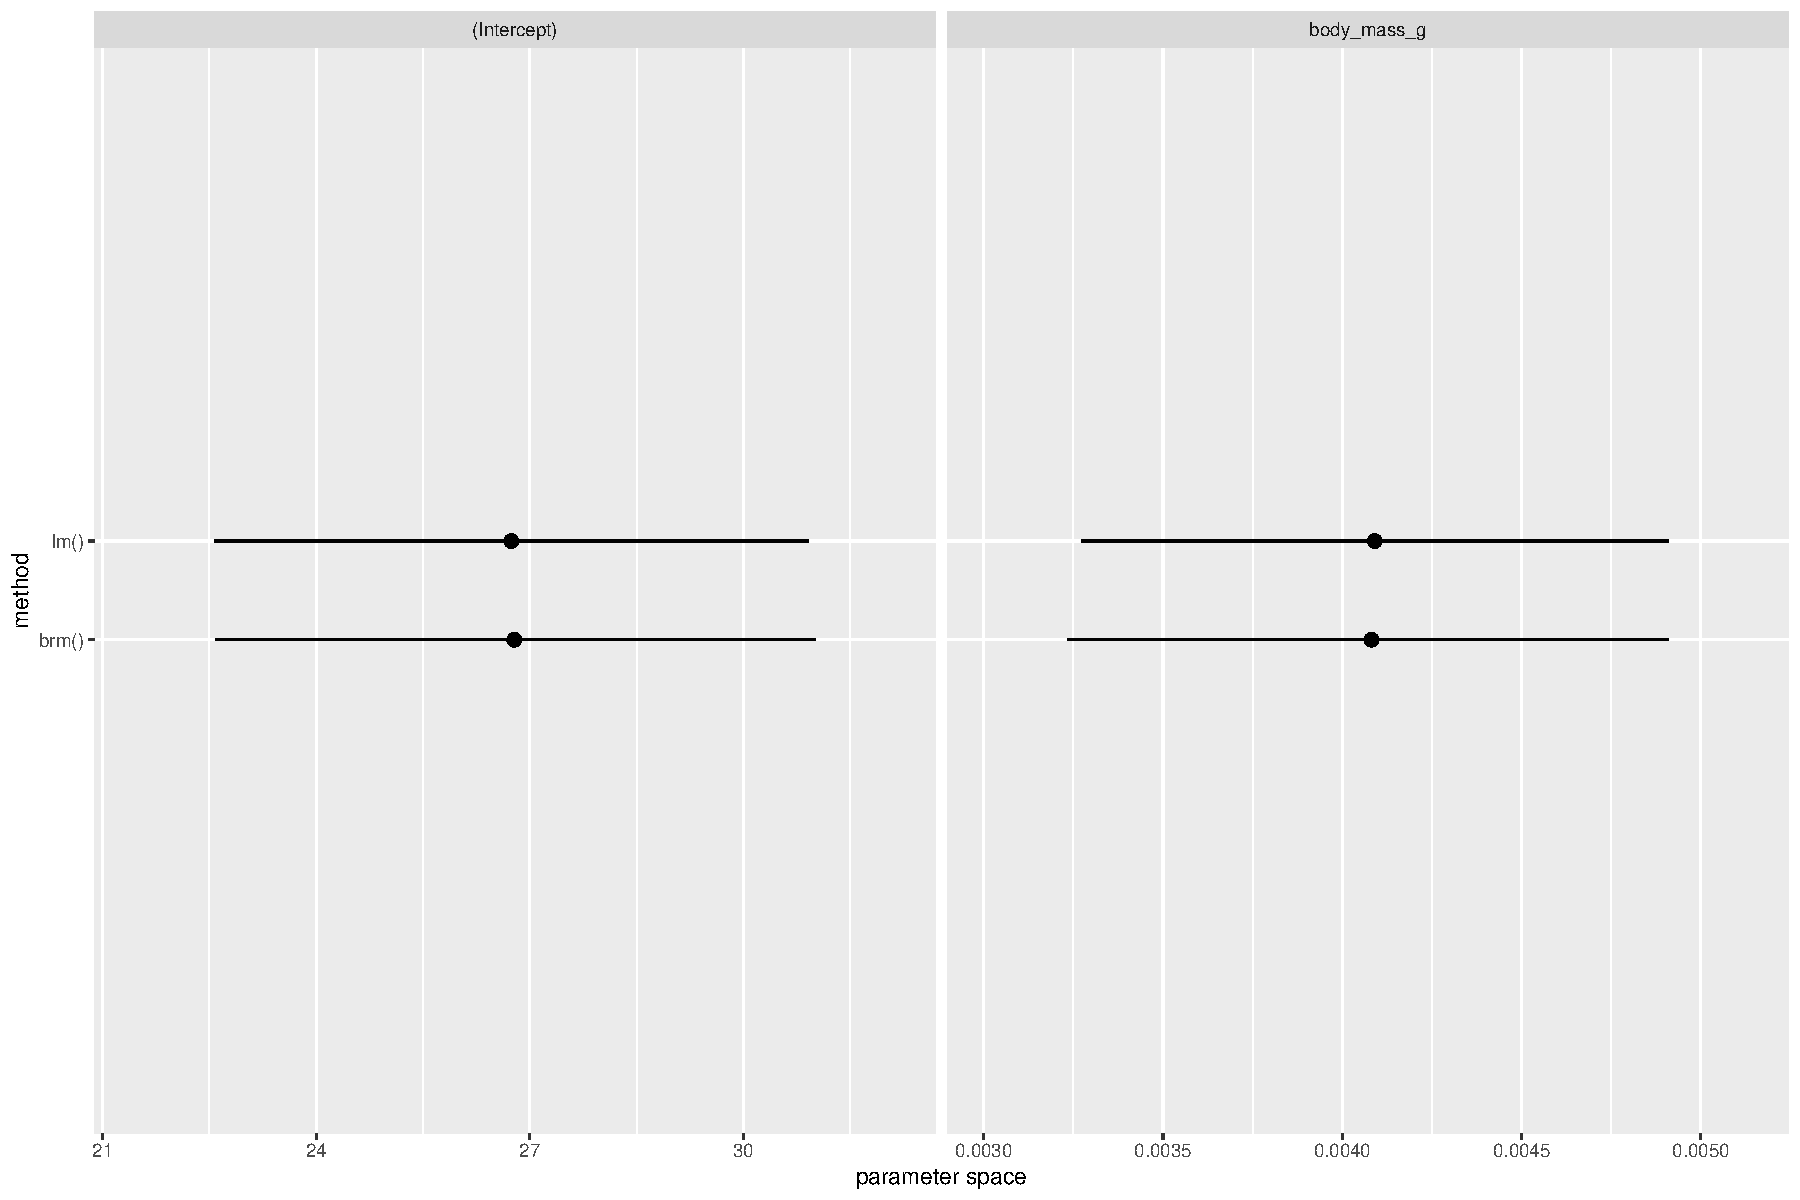
\includegraphics{Bayes_Lab_1_files/figure-pdf/unnamed-chunk-32-1.pdf}

\section{Part 2: Penguins and their
posteriors}\label{part-2-penguins-and-their-posteriors}

\subsection{Exploring model results}\label{exploring-model-results}

We can extract the posterior draws from our Bayesian models with the
\texttt{as\_draws\_df()} function.

\begin{Shaded}
\begin{Highlighting}[]
\FunctionTok{as\_draws\_df}\NormalTok{(fit1.b)}
\end{Highlighting}
\end{Shaded}

\begin{verbatim}
# A draws_df: 1000 iterations, 4 chains, and 6 variables
   b_Intercept b_body_mass_g sigma Intercept lprior lp__
1           32        0.0044   3.3        49   -4.4 -172
2           30        0.0050   3.1        49   -4.4 -172
3           33        0.0043   2.5        49   -4.2 -172
4           33        0.0043   2.5        49   -4.2 -172
5           32        0.0045   2.8        49   -4.3 -171
6           31        0.0047   2.6        49   -4.2 -172
7           33        0.0042   2.8        49   -4.3 -171
8           32        0.0044   2.9        49   -4.3 -171
9           31        0.0048   3.0        49   -4.3 -171
10          32        0.0045   2.9        49   -4.3 -171
# ... with 3990 more draws
# ... hidden reserved variables {'.chain', '.iteration', '.draw'}
\end{verbatim}

Note the meta data. We can get a sense of the full posterior
distributions of the \(\beta\) parameters with plots.

\begin{Shaded}
\begin{Highlighting}[]
\CommentTok{\# wrangle}
\FunctionTok{as\_draws\_df}\NormalTok{(fit1.b) }\SpecialCharTok{\%\textgreater{}\%} 
  \FunctionTok{pivot\_longer}\NormalTok{(}\FunctionTok{starts\_with}\NormalTok{(}\StringTok{"b\_"}\NormalTok{)) }\SpecialCharTok{\%\textgreater{}\%} 
  
  \CommentTok{\# plot!}
  \FunctionTok{ggplot}\NormalTok{(}\FunctionTok{aes}\NormalTok{(}\AttributeTok{x =}\NormalTok{ value)) }\SpecialCharTok{+} 
  \CommentTok{\# geom\_density(fill = "grey20") +}
  \FunctionTok{geom\_histogram}\NormalTok{(}\AttributeTok{bins =} \DecValTok{40}\NormalTok{) }\SpecialCharTok{+}
  \FunctionTok{facet\_wrap}\NormalTok{(}\SpecialCharTok{\textasciitilde{}}\NormalTok{ name, }\AttributeTok{scales =} \StringTok{"free"}\NormalTok{)}
\end{Highlighting}
\end{Shaded}

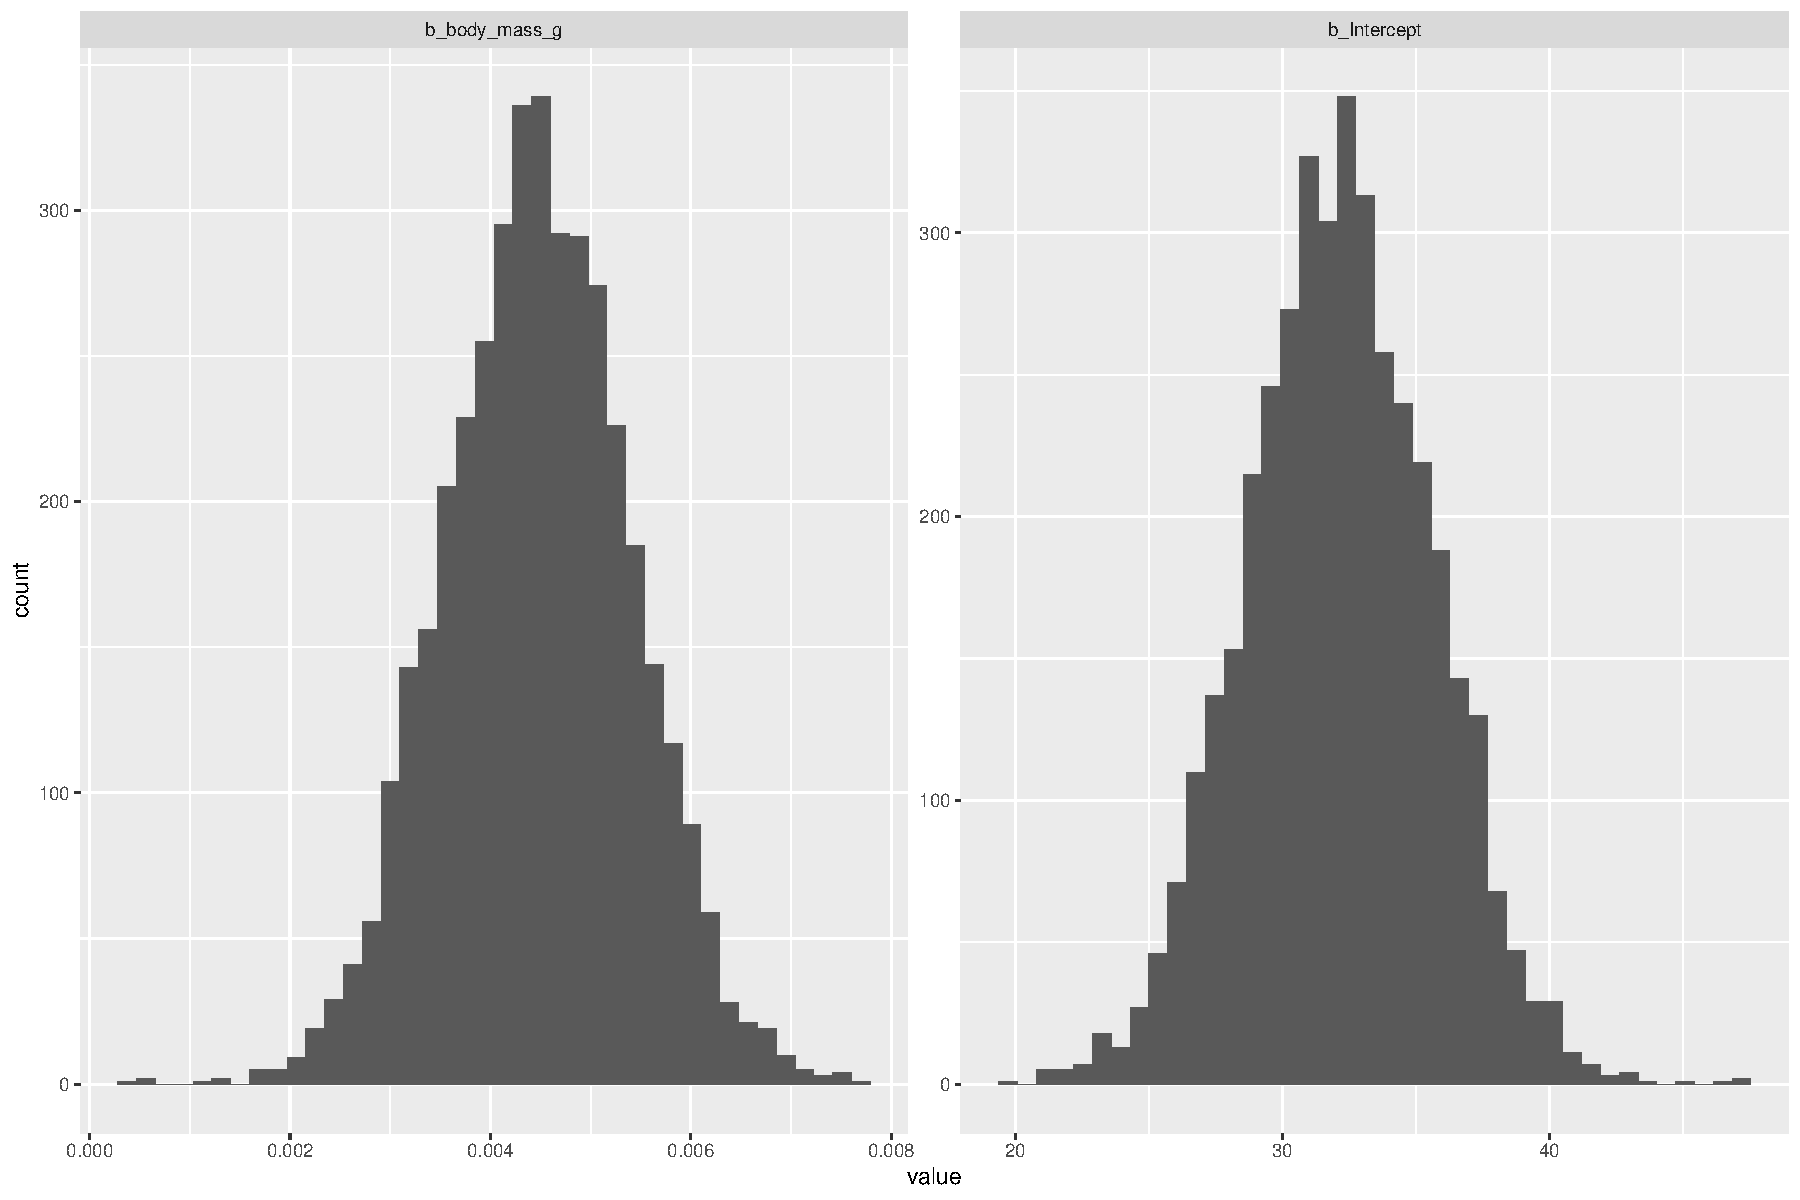
\includegraphics{Bayes_Lab_1_files/figure-pdf/unnamed-chunk-34-1.pdf}

We might summarize those posterior distributions with basic descriptive
statistics, like their means, SD's, and inner 95-percentile range.

\begin{Shaded}
\begin{Highlighting}[]
\FunctionTok{as\_draws\_df}\NormalTok{(fit1.b) }\SpecialCharTok{\%\textgreater{}\%} 
  \FunctionTok{pivot\_longer}\NormalTok{(}\FunctionTok{starts\_with}\NormalTok{(}\StringTok{"b\_"}\NormalTok{)) }\SpecialCharTok{\%\textgreater{}\%} 
  \FunctionTok{group\_by}\NormalTok{(name) }\SpecialCharTok{\%\textgreater{}\%} 
  \FunctionTok{summarise}\NormalTok{(}\AttributeTok{mean =} \FunctionTok{mean}\NormalTok{(value),}
            \AttributeTok{sd =} \FunctionTok{sd}\NormalTok{(value),}
            \AttributeTok{ll =} \FunctionTok{quantile}\NormalTok{(value, }\AttributeTok{probs =} \FloatTok{0.025}\NormalTok{),}
            \AttributeTok{ul =} \FunctionTok{quantile}\NormalTok{(value, }\AttributeTok{probs =} \FloatTok{0.975}\NormalTok{))}
\end{Highlighting}
\end{Shaded}

\begin{verbatim}
# A tibble: 2 x 5
  name              mean       sd       ll       ul
  <chr>            <dbl>    <dbl>    <dbl>    <dbl>
1 b_Intercept   32.1     3.50     25.4     38.9    
2 b_body_mass_g  0.00447 0.000932  0.00268  0.00625
\end{verbatim}

Notice how these values match up exactly with those from
\texttt{fixef()}.

\begin{Shaded}
\begin{Highlighting}[]
\FunctionTok{fixef}\NormalTok{(fit1.b)}
\end{Highlighting}
\end{Shaded}

\begin{verbatim}
                Estimate    Est.Error         Q2.5        Q97.5
Intercept   32.139661018 3.4974943137 25.449370922 38.886468789
body_mass_g  0.004471587 0.0009315803  0.002675154  0.006246179
\end{verbatim}

Thus,

\begin{itemize}
\tightlist
\item
  The Bayesian posterior mean is analogous to the frequentist point
  estimate.
\item
  The Bayesian posterior SD is analogous to the frequentist standard
  error.
\item
  The Bayesian posterior percentile-based 95\% (credible) interval is
  analogous to the frequentist 95\% confidence interval.
\end{itemize}

These are not exactly the same, mind you. But they serve similar
functions.

We can also get a sense of these distributions with the \texttt{plot()}
function.

\begin{Shaded}
\begin{Highlighting}[]
\FunctionTok{plot}\NormalTok{(fit1.b)}
\end{Highlighting}
\end{Shaded}

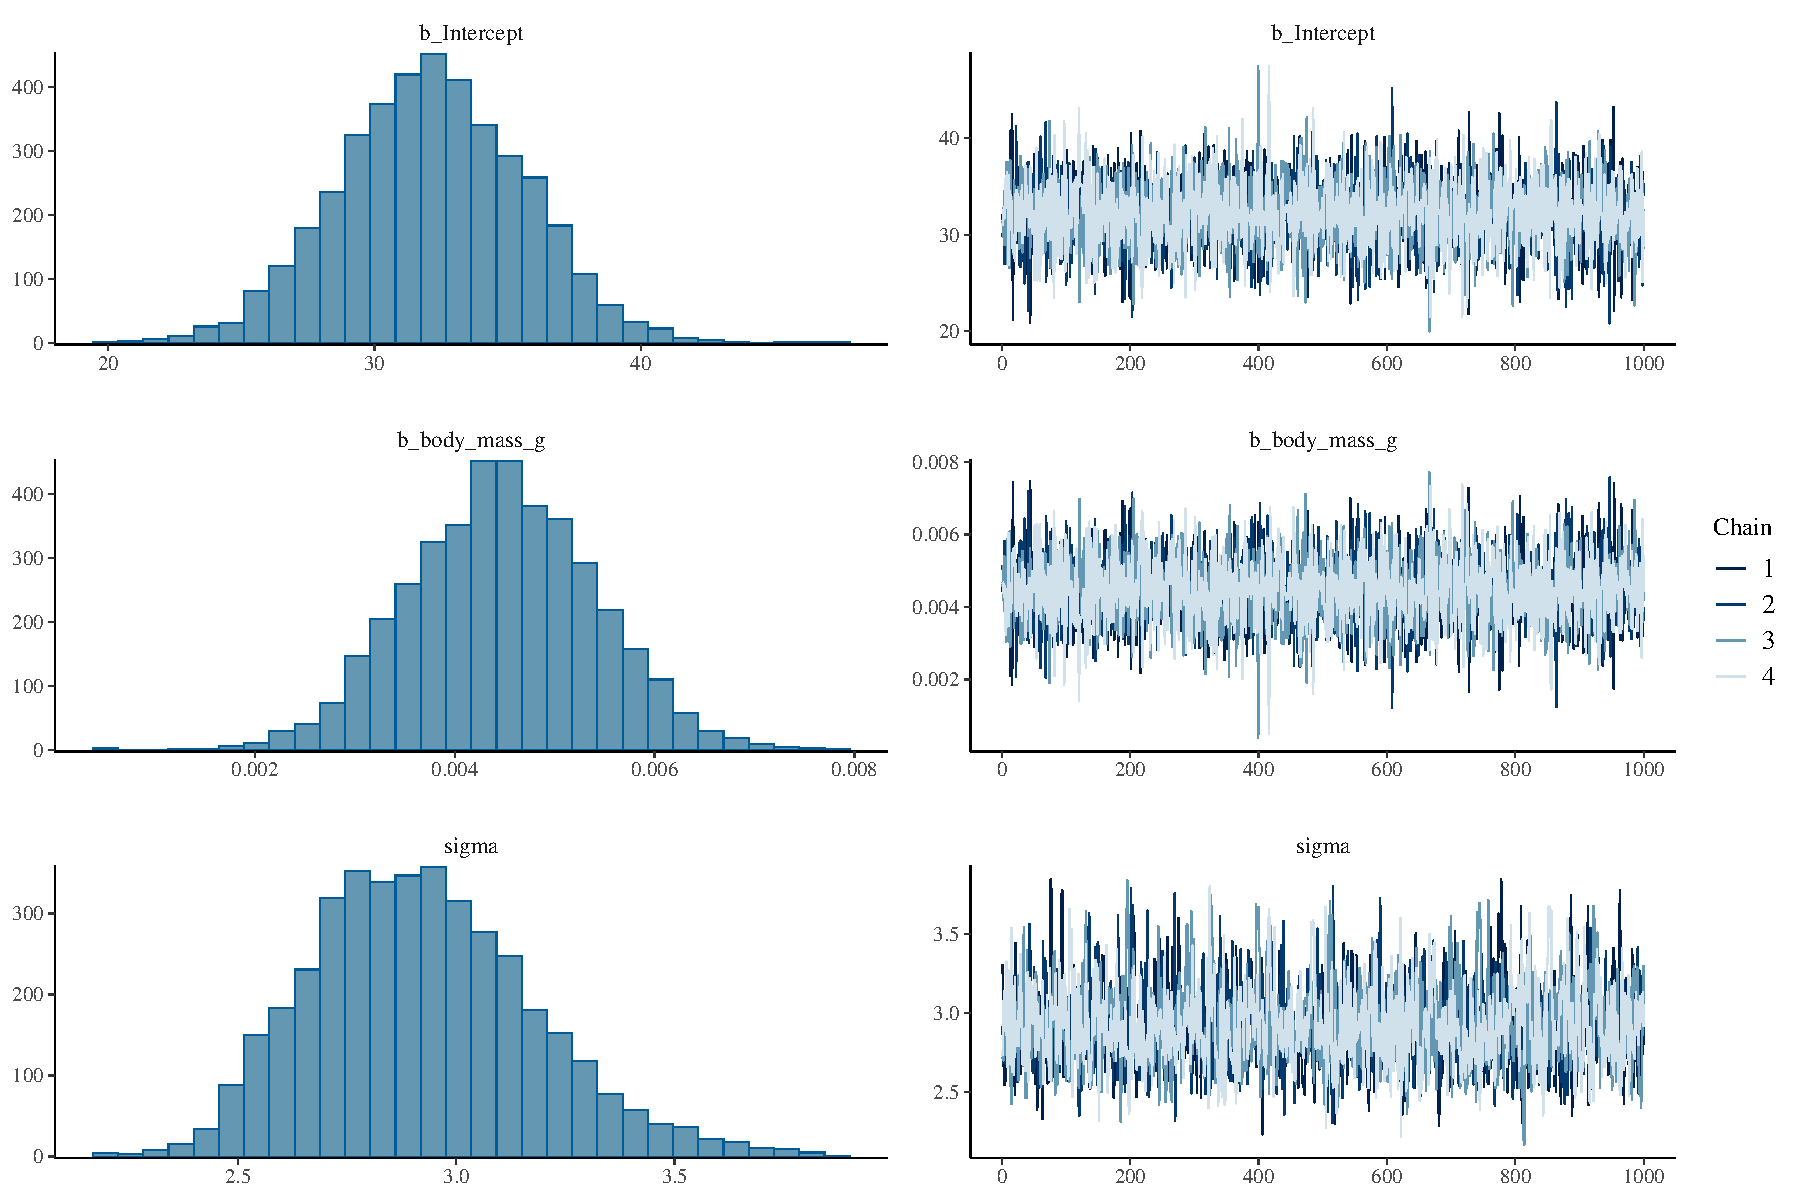
\includegraphics{Bayes_Lab_1_files/figure-pdf/unnamed-chunk-37-1.pdf}

Ignore the trace plots on the right for a moment. And let's consider the
\texttt{pairs()} plot.

\begin{Shaded}
\begin{Highlighting}[]
\FunctionTok{pairs}\NormalTok{(fit1.b)}
\end{Highlighting}
\end{Shaded}

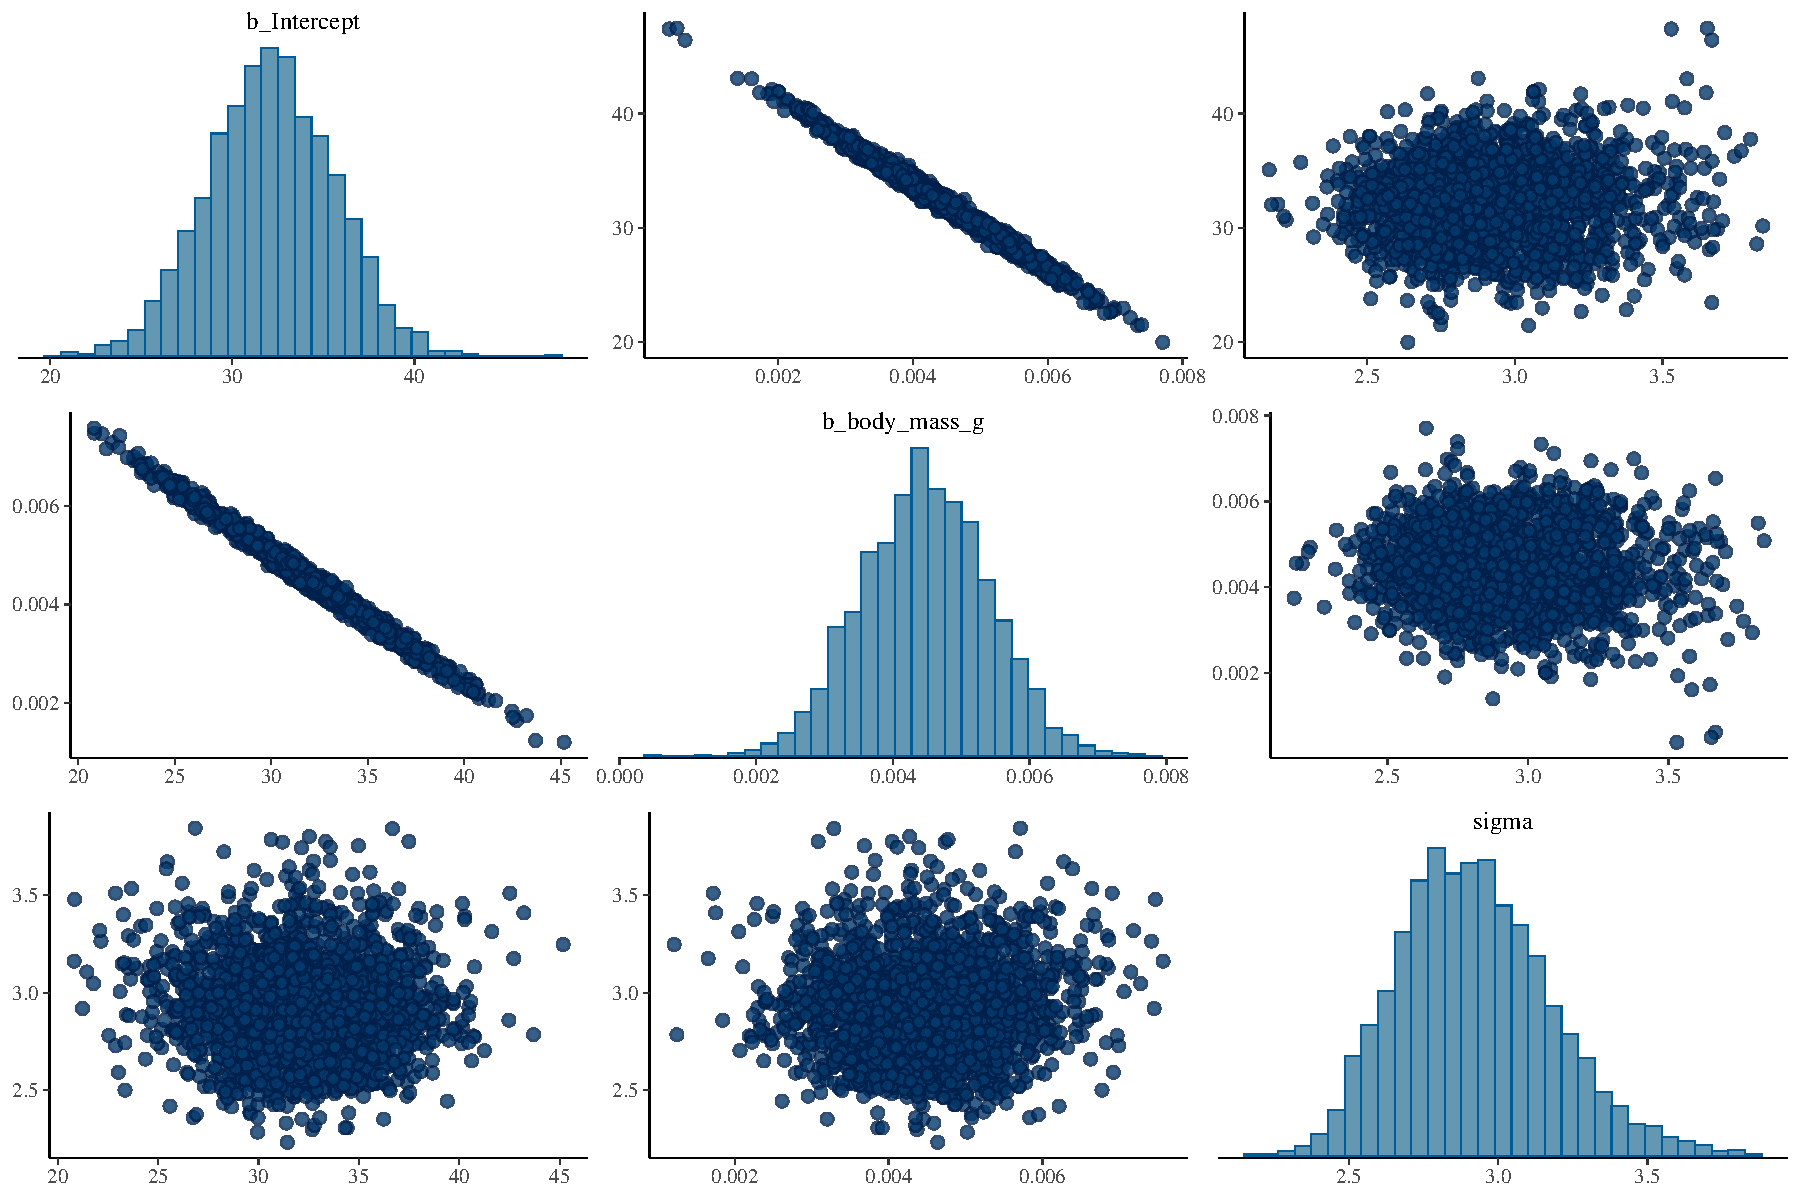
\includegraphics{Bayes_Lab_1_files/figure-pdf/unnamed-chunk-38-1.pdf}

\begin{Shaded}
\begin{Highlighting}[]
\CommentTok{\# we can adjust some of the settings with the off\_diag\_args argument}
\FunctionTok{pairs}\NormalTok{(fit1.b, }\AttributeTok{off\_diag\_args =} \FunctionTok{list}\NormalTok{(}\AttributeTok{size =} \DecValTok{1}\SpecialCharTok{/}\DecValTok{4}\NormalTok{, }\AttributeTok{alpha =} \DecValTok{1}\SpecialCharTok{/}\DecValTok{4}\NormalTok{))}
\end{Highlighting}
\end{Shaded}

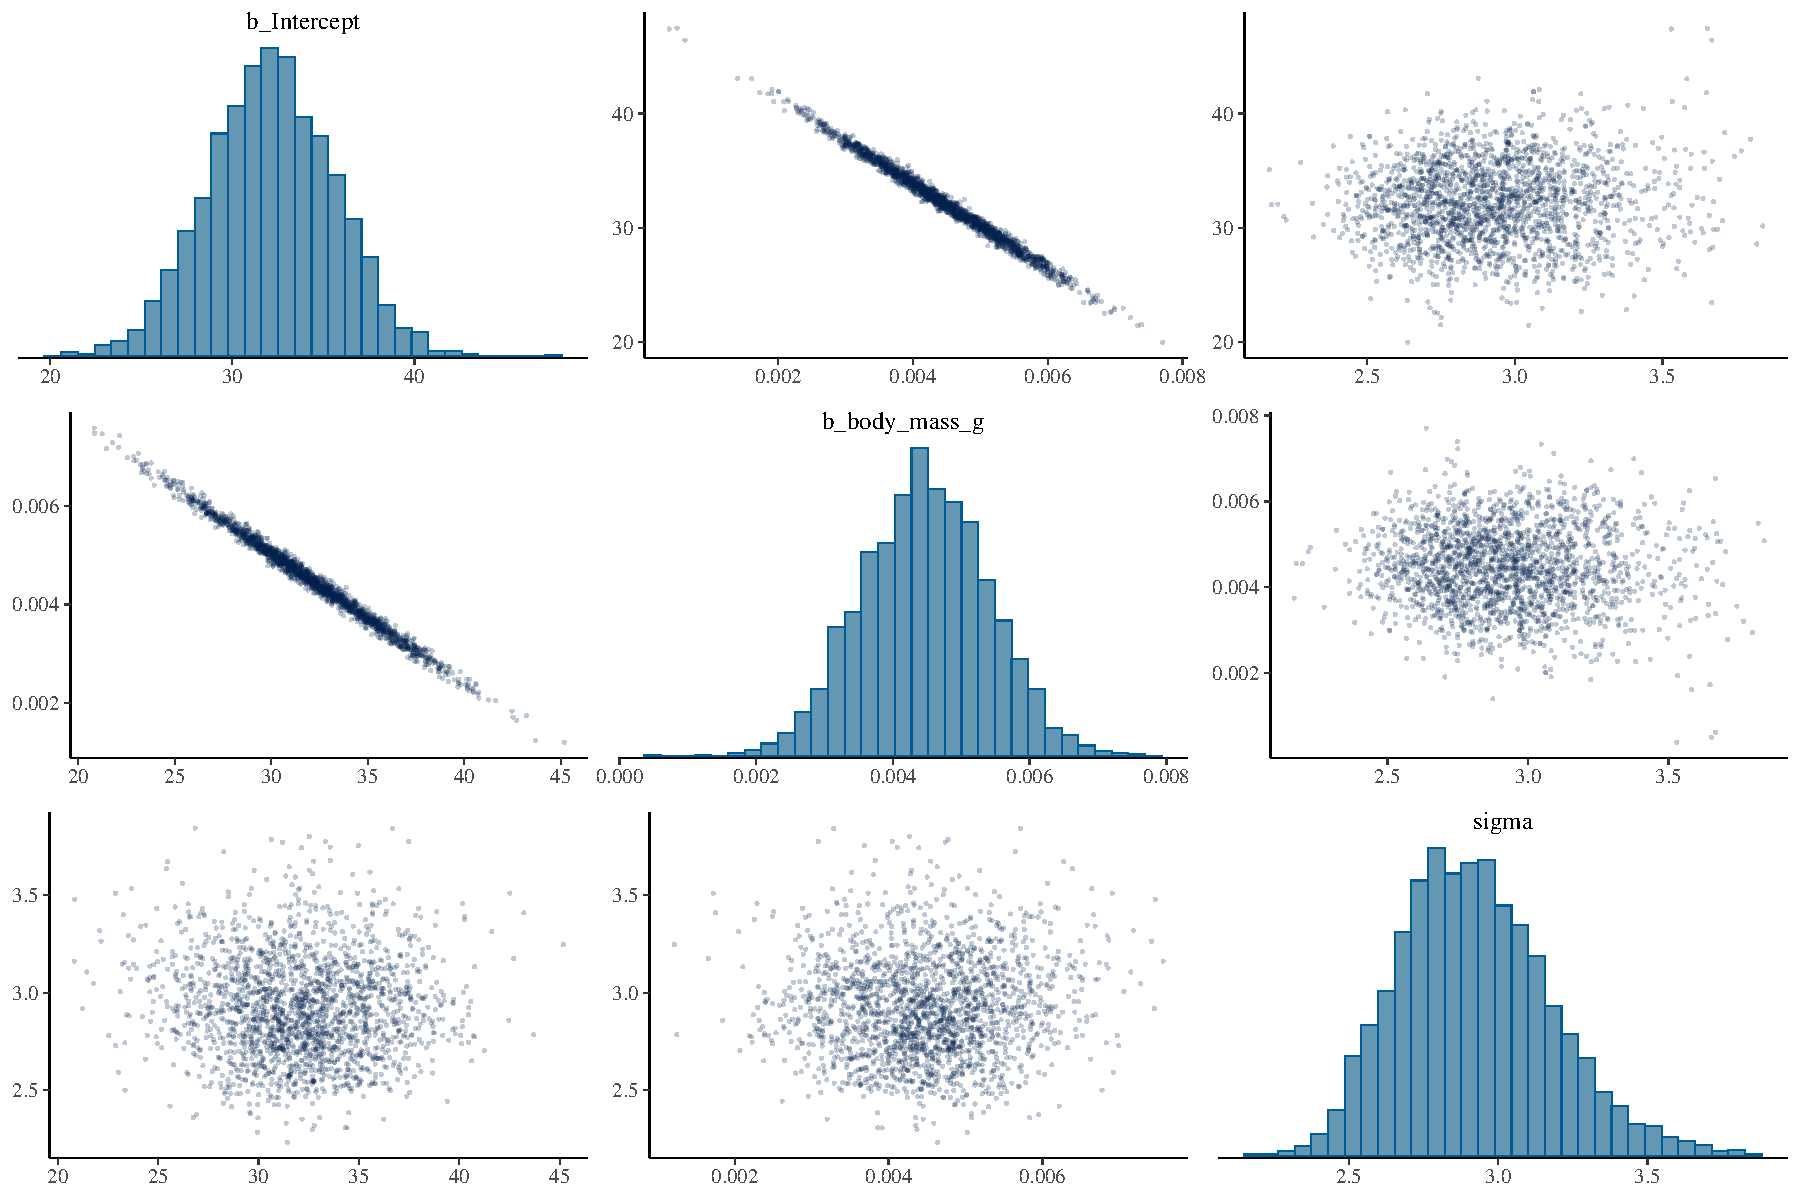
\includegraphics{Bayes_Lab_1_files/figure-pdf/unnamed-chunk-38-2.pdf}

\subsubsection{Question 2.1 : In the parlance of Probability, do you
know what is the term by which the distributions in the diagonal of the
above plot are known as? And the distributions in the
off-diagonal?}\label{question-2.1-in-the-parlance-of-probability-do-you-know-what-is-the-term-by-which-the-distributions-in-the-diagonal-of-the-above-plot-are-known-as-and-the-distributions-in-the-off-diagonal}

\begin{verbatim}
The diagonal ones are the marginal distributions of individual parameters.

The off-diagnoal ones are the bivariate marginal distributions, or the joint distributions of the paired two parameters, marginalized over the remaining parameters.
\end{verbatim}

Notice how the two \(\beta\) parameters seem to have a strong negative
correlation. We can quantify that correlation with the \texttt{vcov()}
function.

\begin{Shaded}
\begin{Highlighting}[]
\FunctionTok{vcov}\NormalTok{(fit1.b)                      }\CommentTok{\# variance/covariance metric}
\end{Highlighting}
\end{Shaded}

\begin{verbatim}
              Intercept   body_mass_g
Intercept   12.23246647 -3.240360e-03
body_mass_g -0.00324036  8.678418e-07
\end{verbatim}

\begin{Shaded}
\begin{Highlighting}[]
\FunctionTok{vcov}\NormalTok{(fit1.b, }\AttributeTok{correlation =} \ConstantTok{TRUE}\NormalTok{)  }\CommentTok{\# correlation metric}
\end{Highlighting}
\end{Shaded}

\begin{verbatim}
             Intercept body_mass_g
Intercept    1.0000000  -0.9945256
body_mass_g -0.9945256   1.0000000
\end{verbatim}

This correlation/covariance among the parameters is not unique to
Bayesian models. Here's the \texttt{vcov()} output for the OLS model.

\begin{Shaded}
\begin{Highlighting}[]
\FunctionTok{vcov}\NormalTok{(fit1.ols)  }\CommentTok{\# variance/covariance metric}
\end{Highlighting}
\end{Shaded}

\begin{verbatim}
             (Intercept)   body_mass_g
(Intercept) 11.856743861 -3.143295e-03
body_mass_g -0.003143295  8.420092e-07
\end{verbatim}

I'm not aware of an easy way to get that output in a correlation metric
for our OLS model. Here's how to compute the correlation by hand.

\begin{Shaded}
\begin{Highlighting}[]
\NormalTok{cov\_xy }\OtherTok{\textless{}{-}} \FunctionTok{vcov}\NormalTok{(fit1.ols)[}\DecValTok{2}\NormalTok{, }\DecValTok{1}\NormalTok{]  }\CommentTok{\# covariance between the intercept and slope}
\NormalTok{var\_x  }\OtherTok{\textless{}{-}} \FunctionTok{vcov}\NormalTok{(fit1.ols)[}\DecValTok{1}\NormalTok{, }\DecValTok{1}\NormalTok{]  }\CommentTok{\# variance for the intercept}
\NormalTok{var\_y  }\OtherTok{\textless{}{-}} \FunctionTok{vcov}\NormalTok{(fit1.ols)[}\DecValTok{2}\NormalTok{, }\DecValTok{2}\NormalTok{]  }\CommentTok{\# variance for the slope}

\CommentTok{\# convert the covariance into a correlation}
\NormalTok{cov\_xy }\SpecialCharTok{/}\NormalTok{ (}\FunctionTok{sqrt}\NormalTok{(var\_x) }\SpecialCharTok{*} \FunctionTok{sqrt}\NormalTok{(var\_y))}
\end{Highlighting}
\end{Shaded}

\begin{verbatim}
[1] -0.9948188
\end{verbatim}

That code follows the definition of a covariance, which can be expressed
as

\[
\text{Cov}(x, y) = \rho \sigma_x \sigma_y,
\]

where \(\sigma_x\) is the standard deviation for x, \(\sigma_y\) is the
standard deviation for y, and \(\rho\) is their correlation. And thus,
you can convert a covariance into a correlation with the formula

\[
\rho = \frac{\sigma_{xy}}{\sigma_x \sigma_y},
\]

where \(\sigma_{xy}\) is the covariance of x and y.

\subsection{Draws}\label{draws}

Let's save the \texttt{as\_draws\_df()} output for our model as an
object called \texttt{draws}.

\begin{Shaded}
\begin{Highlighting}[]
\NormalTok{draws }\OtherTok{\textless{}{-}} \FunctionTok{as\_draws\_df}\NormalTok{(fit1.b)}
\FunctionTok{glimpse}\NormalTok{(draws)}
\end{Highlighting}
\end{Shaded}

\begin{verbatim}
Rows: 4,000
Columns: 9
$ b_Intercept   <dbl> 32.04902, 29.82826, 32.75581, 32.75581, 31.90975, 31.428~
$ b_body_mass_g <dbl> 0.004416532, 0.005004505, 0.004315146, 0.004315146, 0.00~
$ sigma         <dbl> 3.305827, 3.074178, 2.546395, 2.546395, 2.817548, 2.5701~
$ Intercept     <dbl> 48.53632, 48.51052, 48.86463, 48.86463, 48.57453, 48.799~
$ lprior        <dbl> -4.413119, -4.355407, -4.199641, -4.199641, -4.285679, -~
$ lp__          <dbl> -172.4514, -171.7148, -171.7431, -171.7431, -171.1050, -~
$ .chain        <int> 1, 1, 1, 1, 1, 1, 1, 1, 1, 1, 1, 1, 1, 1, 1, 1, 1, 1, 1,~
$ .iteration    <int> 1, 2, 3, 4, 5, 6, 7, 8, 9, 10, 11, 12, 13, 14, 15, 16, 1~
$ .draw         <int> 1, 2, 3, 4, 5, 6, 7, 8, 9, 10, 11, 12, 13, 14, 15, 16, 1~
\end{verbatim}

For each parameter in the model, we have 4,000 draws from the posterior.

\subsubsection{Question 2.2: How does this concept relate to
representing uncertainty? Can you anticipate how predictions are made
based upon these 4000 draws and the linear regression
formula?}\label{question-2.2-how-does-this-concept-relate-to-representing-uncertainty-can-you-anticipate-how-predictions-are-made-based-upon-these-4000-draws-and-the-linear-regression-formula}

\begin{verbatim}
Since we hae 4000 posterior samples, the spread can tell us how uncertain we are about each parameter. We can also get the mean and the 95% confidence interval from the distribution.

For each value of x, the predictions are made by averaging the predicted values across the 4000 samples of the parameters.
\end{verbatim}

\[
\widehat{\text{bill_length_mm}}_i = \beta_0 + \beta_1 \text{body_mass_g}_i.
\]

Let's break the 4000 draws down with our \texttt{draws} object.

\begin{Shaded}
\begin{Highlighting}[]
\CommentTok{\# adjust the parameter names }
\NormalTok{draws }\OtherTok{\textless{}{-}}\NormalTok{ draws }\SpecialCharTok{\%\textgreater{}\%} 
  \FunctionTok{mutate}\NormalTok{(}\AttributeTok{beta0 =}\NormalTok{ b\_Intercept,}
         \AttributeTok{beta1 =}\NormalTok{ b\_body\_mass\_g)}

\CommentTok{\# Note: go through this one line at a time}
\NormalTok{draws }\SpecialCharTok{\%\textgreater{}\%} 
  \FunctionTok{select}\NormalTok{(.draw, beta0, beta1) }\SpecialCharTok{\%\textgreater{}\%} 
  \FunctionTok{mutate}\NormalTok{(}\AttributeTok{body\_mass\_g =} \FunctionTok{mean}\NormalTok{(chinstrap}\SpecialCharTok{$}\NormalTok{body\_mass\_g)) }\SpecialCharTok{\%\textgreater{}\%} 
  \FunctionTok{mutate}\NormalTok{(}\AttributeTok{y\_hat =}\NormalTok{ beta0 }\SpecialCharTok{+}\NormalTok{ beta1 }\SpecialCharTok{*}\NormalTok{ body\_mass\_g) }\SpecialCharTok{\%\textgreater{}\%} 
  
  \FunctionTok{ggplot}\NormalTok{(}\FunctionTok{aes}\NormalTok{(}\AttributeTok{x =}\NormalTok{ y\_hat)) }\SpecialCharTok{+}
  \FunctionTok{geom\_histogram}\NormalTok{(}\AttributeTok{bins =} \DecValTok{40}\NormalTok{) }\SpecialCharTok{+}
  \FunctionTok{labs}\NormalTok{(}\AttributeTok{title =} \StringTok{"Bayesians have posterior distributions"}\NormalTok{,}
       \AttributeTok{x =} \FunctionTok{expression}\NormalTok{(}\FunctionTok{hat}\NormalTok{(}\FunctionTok{italic}\NormalTok{(y))}\SpecialCharTok{*}\StringTok{\textquotesingle{}|\textquotesingle{}}\SpecialCharTok{*}\FunctionTok{italic}\NormalTok{(x)}\SpecialCharTok{==}\FloatTok{3733.1}\NormalTok{)) }\SpecialCharTok{+}
  \FunctionTok{coord\_cartesian}\NormalTok{(}\AttributeTok{xlim =} \FunctionTok{c}\NormalTok{(}\DecValTok{47}\NormalTok{, }\DecValTok{51}\NormalTok{))}
\end{Highlighting}
\end{Shaded}

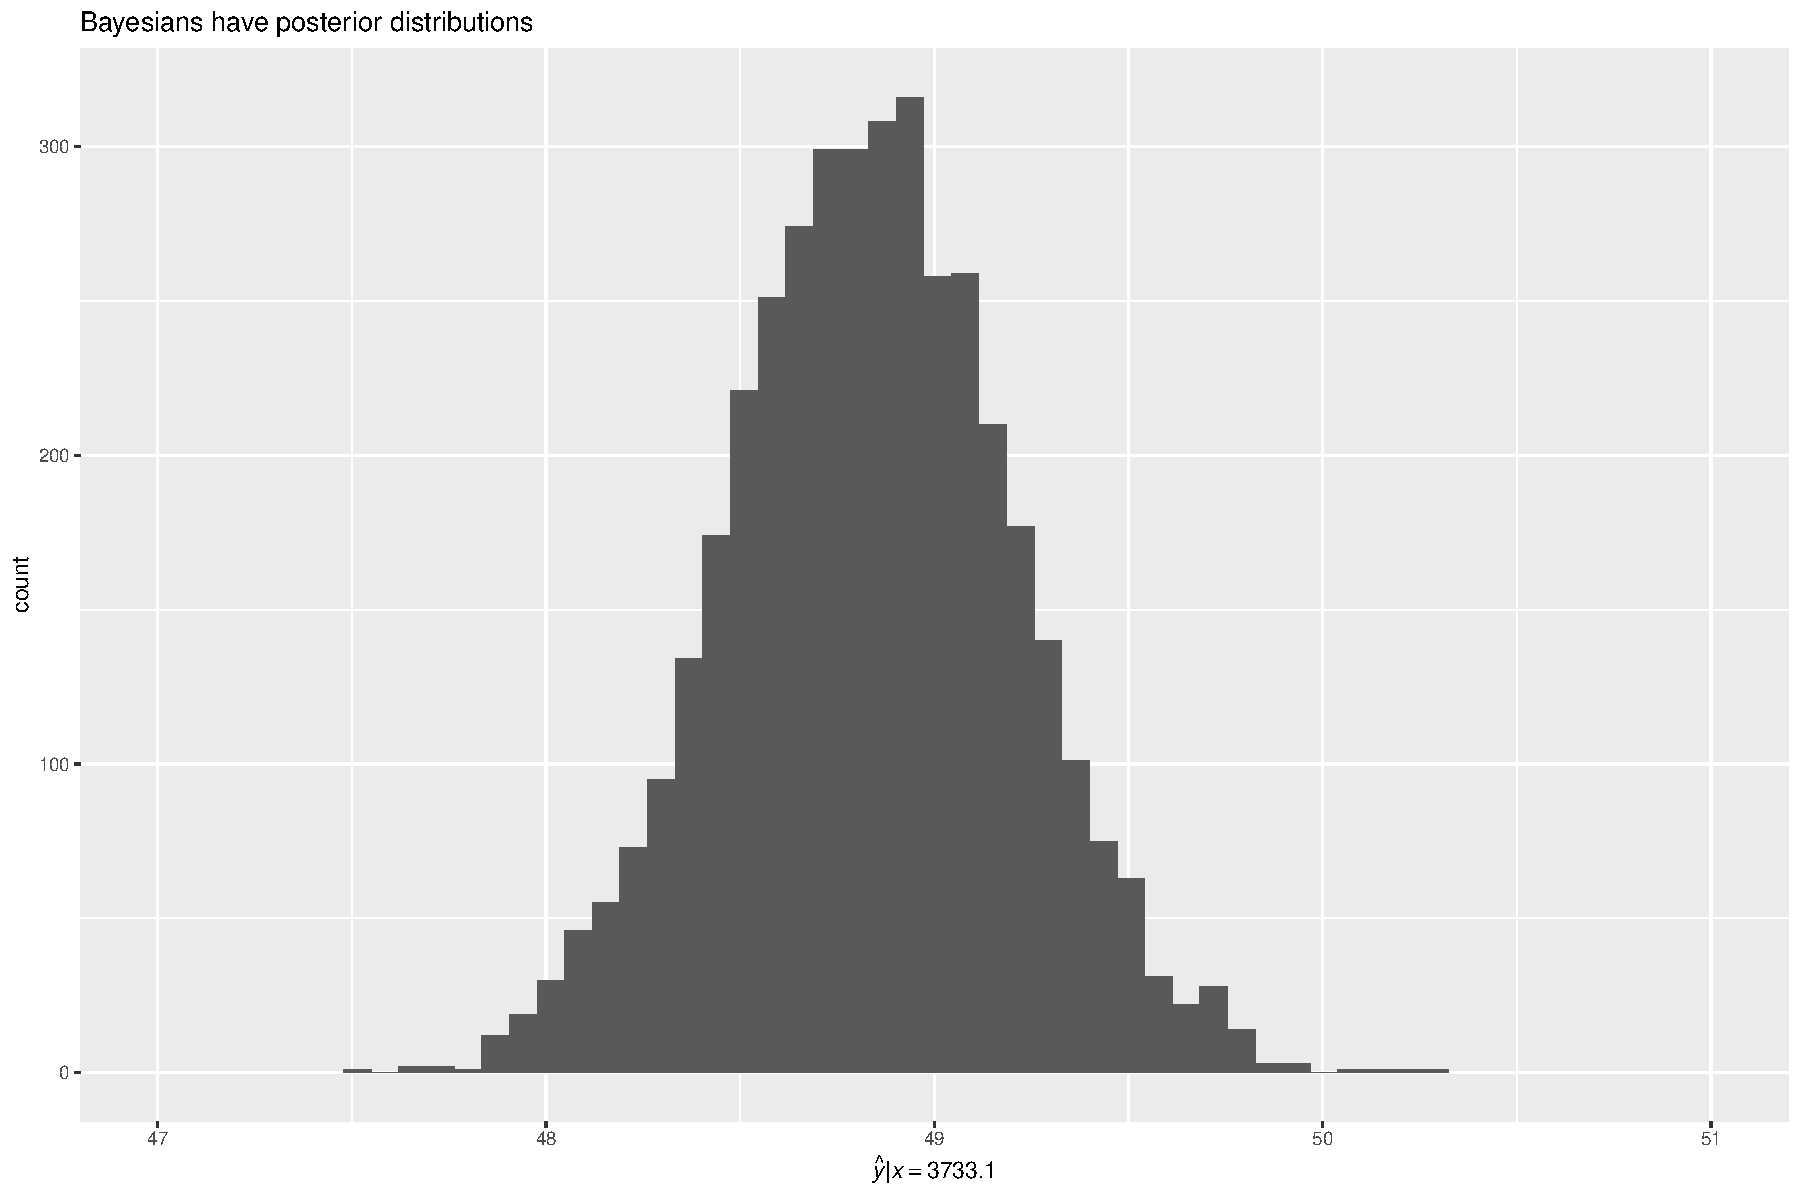
\includegraphics{Bayes_Lab_1_files/figure-pdf/unnamed-chunk-43-1.pdf}

Here's what that is for the OLS model.

\begin{Shaded}
\begin{Highlighting}[]
\FunctionTok{predict}\NormalTok{(fit1.ols,}
        \AttributeTok{newdata =} \FunctionTok{tibble}\NormalTok{(}\AttributeTok{body\_mass\_g =} \FunctionTok{mean}\NormalTok{(chinstrap}\SpecialCharTok{$}\NormalTok{body\_mass\_g)),}
        \AttributeTok{interval =} \StringTok{"confidence"}\NormalTok{) }\SpecialCharTok{\%\textgreater{}\%} 
  \FunctionTok{data.frame}\NormalTok{() }\SpecialCharTok{\%\textgreater{}\%} 
  
  \FunctionTok{ggplot}\NormalTok{(}\FunctionTok{aes}\NormalTok{(}\AttributeTok{x =}\NormalTok{ fit, }\AttributeTok{xmin =}\NormalTok{ lwr, }\AttributeTok{xmax =}\NormalTok{ upr, }\AttributeTok{y =} \DecValTok{0}\NormalTok{)) }\SpecialCharTok{+}
  \FunctionTok{geom\_pointrange}\NormalTok{() }\SpecialCharTok{+}
  \FunctionTok{scale\_y\_continuous}\NormalTok{(}\ConstantTok{NULL}\NormalTok{, }\AttributeTok{breaks =} \ConstantTok{NULL}\NormalTok{) }\SpecialCharTok{+}
  \FunctionTok{labs}\NormalTok{(}\AttributeTok{title =} \StringTok{"Frequentists have point estmates and 95\% CI\textquotesingle{}s"}\NormalTok{,}
       \AttributeTok{x =} \FunctionTok{expression}\NormalTok{(}\FunctionTok{hat}\NormalTok{(}\FunctionTok{italic}\NormalTok{(y))}\SpecialCharTok{*}\StringTok{\textquotesingle{}|\textquotesingle{}}\SpecialCharTok{*}\FunctionTok{italic}\NormalTok{(x)}\SpecialCharTok{==}\FloatTok{3733.1}\NormalTok{)) }\SpecialCharTok{+}
  \FunctionTok{coord\_cartesian}\NormalTok{(}\AttributeTok{xlim =} \FunctionTok{c}\NormalTok{(}\DecValTok{47}\NormalTok{, }\DecValTok{51}\NormalTok{))}
\end{Highlighting}
\end{Shaded}

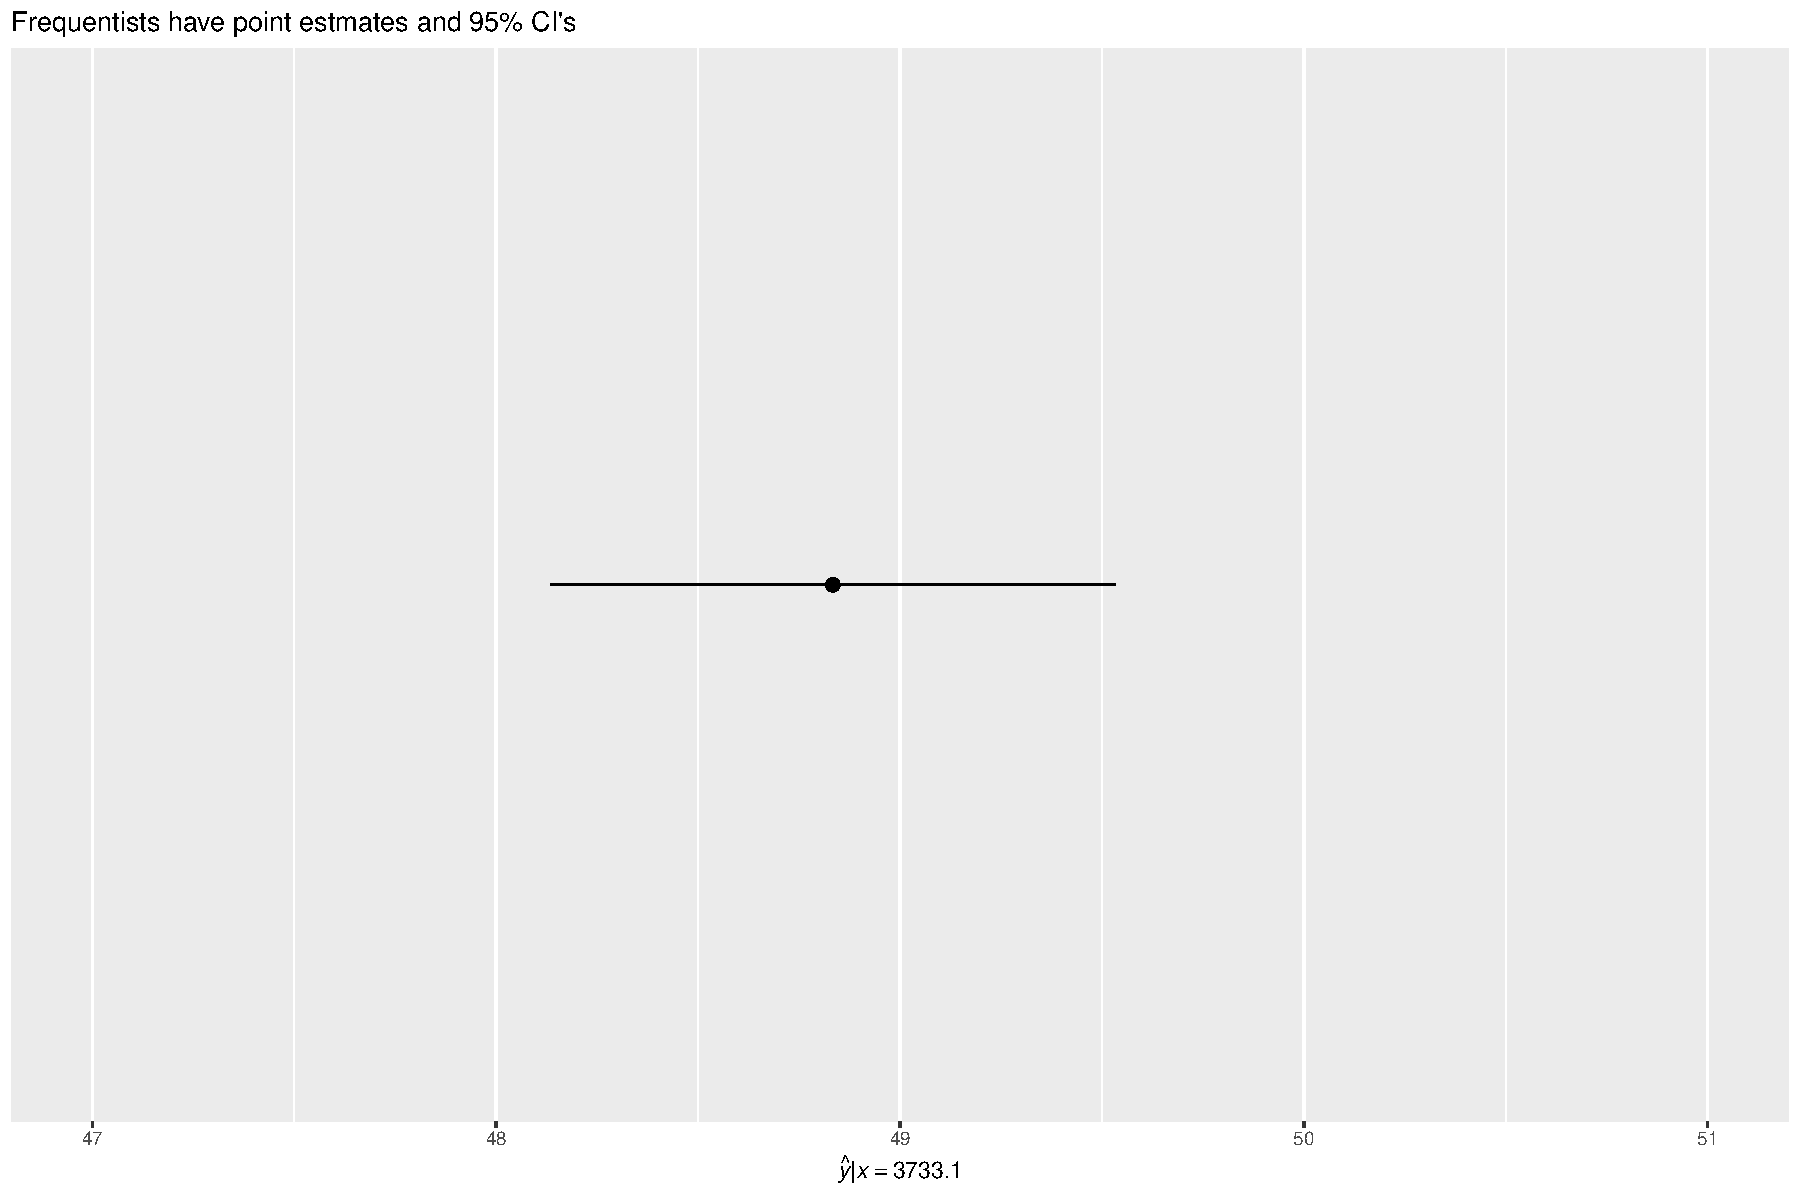
\includegraphics{Bayes_Lab_1_files/figure-pdf/unnamed-chunk-44-1.pdf}

Another handy way to present a Bayesian posterior is as a density with a
point-interval summary below.

\begin{Shaded}
\begin{Highlighting}[]
\FunctionTok{library}\NormalTok{(ggdist) }\CommentTok{\#for stat\_half\_eye and mean\_qi}
\NormalTok{draws }\SpecialCharTok{\%\textgreater{}\%} 
  \FunctionTok{mutate}\NormalTok{(}\AttributeTok{body\_mass\_g =} \FunctionTok{mean}\NormalTok{(chinstrap}\SpecialCharTok{$}\NormalTok{body\_mass\_g)) }\SpecialCharTok{\%\textgreater{}\%} 
  \FunctionTok{mutate}\NormalTok{(}\AttributeTok{y\_hat =}\NormalTok{ beta0 }\SpecialCharTok{+}\NormalTok{ beta1 }\SpecialCharTok{*}\NormalTok{ body\_mass\_g) }\SpecialCharTok{\%\textgreater{}\%} 
  
  \FunctionTok{ggplot}\NormalTok{(}\FunctionTok{aes}\NormalTok{(}\AttributeTok{x =}\NormalTok{ y\_hat)) }\SpecialCharTok{+}
  \FunctionTok{stat\_halfeye}\NormalTok{(}\AttributeTok{point\_interval =}\NormalTok{ mean\_qi, }\AttributeTok{.width =}\NormalTok{ .}\DecValTok{95}\NormalTok{) }\SpecialCharTok{+}
  \CommentTok{\# scale\_y\_continuous(NULL, breaks = NULL) +}
  \FunctionTok{labs}\NormalTok{(}\AttributeTok{title =} \StringTok{"Bayesians have posterior distributions"}\NormalTok{,}
       \AttributeTok{x =} \FunctionTok{expression}\NormalTok{(}\FunctionTok{hat}\NormalTok{(}\FunctionTok{italic}\NormalTok{(y))}\SpecialCharTok{*}\StringTok{\textquotesingle{}|\textquotesingle{}}\SpecialCharTok{*}\FunctionTok{italic}\NormalTok{(x)}\SpecialCharTok{==}\FloatTok{3733.1}\NormalTok{)) }\SpecialCharTok{+}
  \FunctionTok{coord\_cartesian}\NormalTok{(}\AttributeTok{xlim =} \FunctionTok{c}\NormalTok{(}\DecValTok{47}\NormalTok{, }\DecValTok{51}\NormalTok{))}
\end{Highlighting}
\end{Shaded}

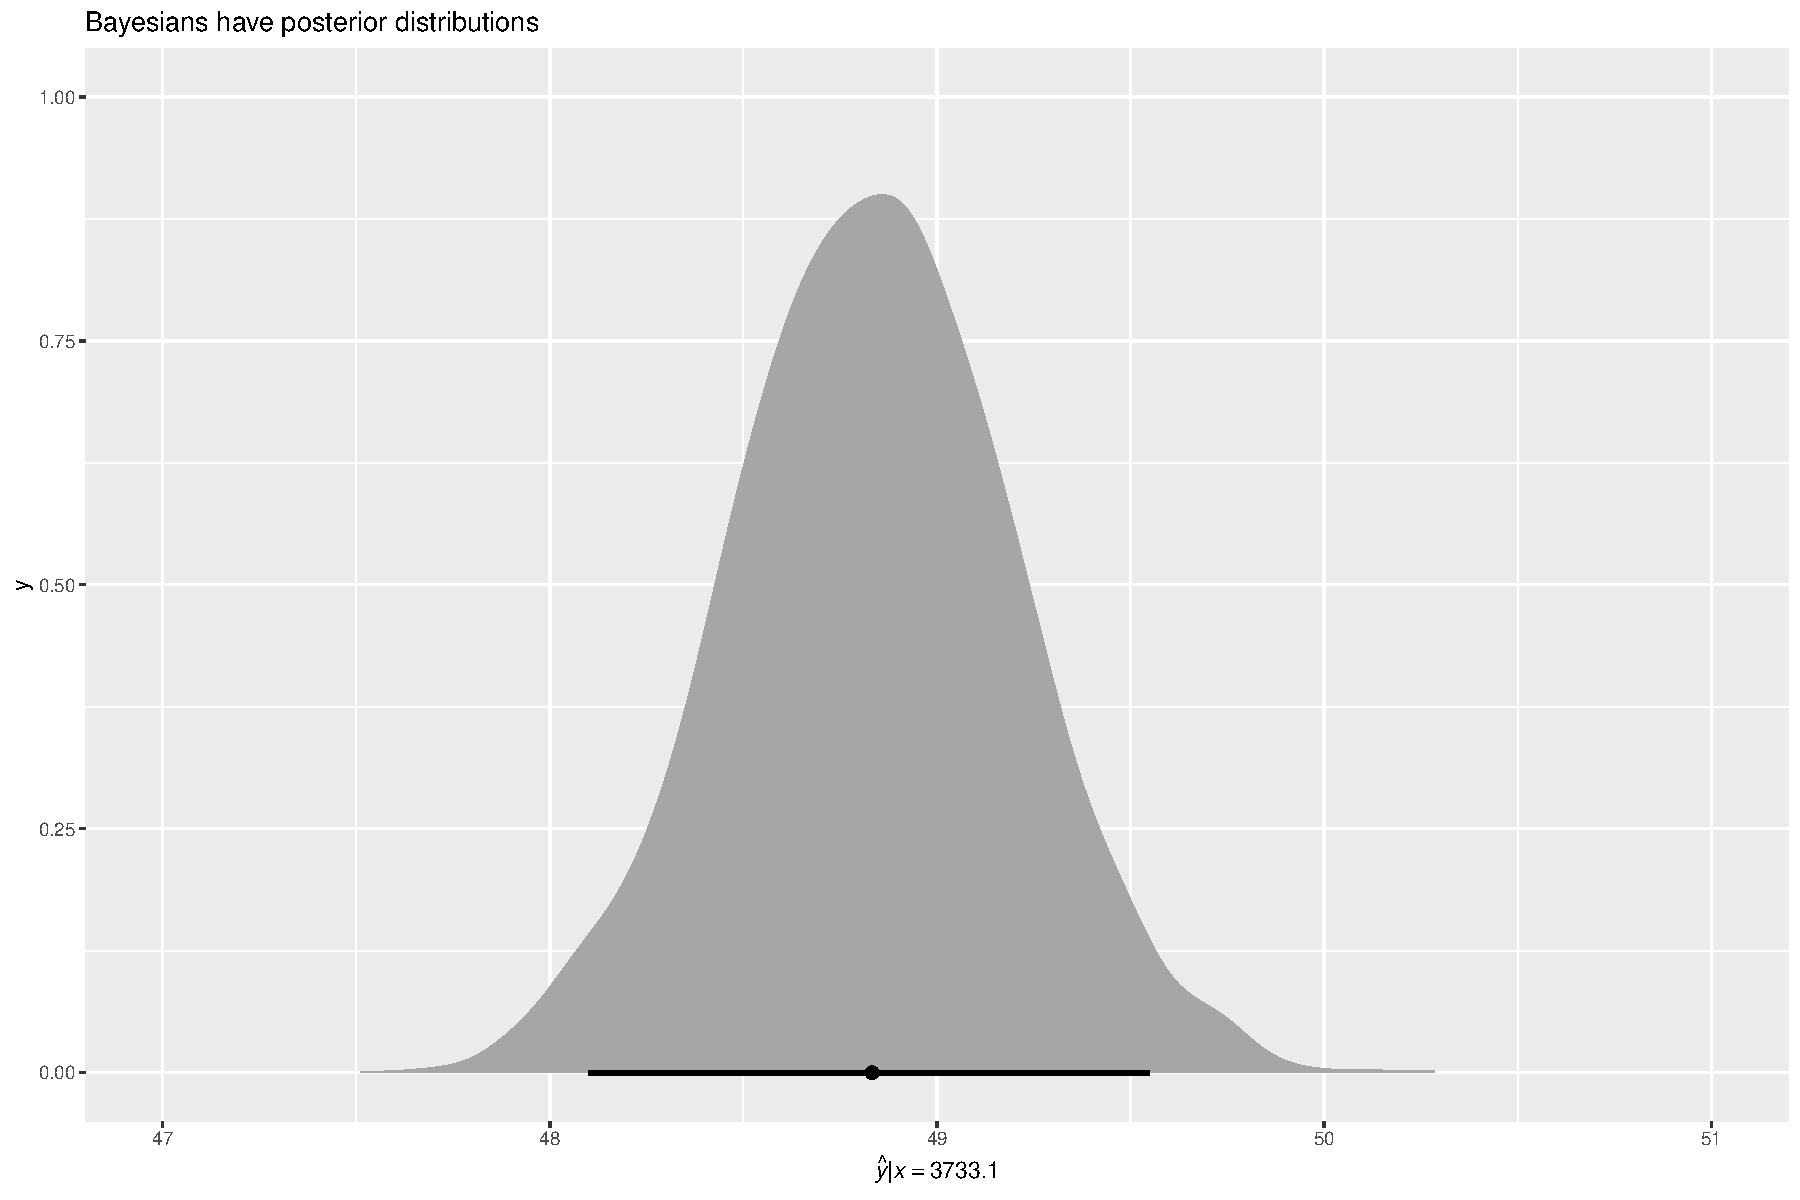
\includegraphics{Bayes_Lab_1_files/figure-pdf/unnamed-chunk-45-1.pdf}

The dot at the base of the plot is the posterior mean, and the
horizontal line marks the 95\% percentile-based interval. If you'd like
to mark the median instead, set \texttt{point\_interval\ =\ median\_qi}.
If you're like a different kind of horizontal interval, adjust the
\texttt{.width} argument.

\begin{Shaded}
\begin{Highlighting}[]
\NormalTok{draws }\SpecialCharTok{\%\textgreater{}\%} 
  \FunctionTok{mutate}\NormalTok{(}\AttributeTok{body\_mass\_g =} \FunctionTok{mean}\NormalTok{(chinstrap}\SpecialCharTok{$}\NormalTok{body\_mass\_g)) }\SpecialCharTok{\%\textgreater{}\%} 
  \FunctionTok{mutate}\NormalTok{(}\AttributeTok{y\_hat =}\NormalTok{ beta0 }\SpecialCharTok{+}\NormalTok{ beta1 }\SpecialCharTok{*}\NormalTok{ body\_mass\_g) }\SpecialCharTok{\%\textgreater{}\%} 
  
  \FunctionTok{ggplot}\NormalTok{(}\FunctionTok{aes}\NormalTok{(}\AttributeTok{x =}\NormalTok{ y\_hat)) }\SpecialCharTok{+}
  \CommentTok{\# note the changes to this line}
  \FunctionTok{stat\_halfeye}\NormalTok{(}\AttributeTok{point\_interval =}\NormalTok{ median\_qi, }\AttributeTok{.width =} \FunctionTok{c}\NormalTok{(.}\DecValTok{5}\NormalTok{, .}\DecValTok{99}\NormalTok{)) }\SpecialCharTok{+}
  \FunctionTok{scale\_y\_continuous}\NormalTok{(}\ConstantTok{NULL}\NormalTok{, }\AttributeTok{breaks =} \ConstantTok{NULL}\NormalTok{) }\SpecialCharTok{+}
  \FunctionTok{labs}\NormalTok{(}\AttributeTok{title =} \StringTok{"Bayesians have posterior distributions"}\NormalTok{,}
       \AttributeTok{subtitle =} \StringTok{"The dot marks the median.}\SpecialCharTok{\textbackslash{}n}\StringTok{The thicker line marks the 50\% interval, and}\SpecialCharTok{\textbackslash{}n}\StringTok{the thinner line marks the 99\% interval."}\NormalTok{,}
       \AttributeTok{x =} \FunctionTok{expression}\NormalTok{(}\FunctionTok{hat}\NormalTok{(}\FunctionTok{italic}\NormalTok{(y))}\SpecialCharTok{*}\StringTok{\textquotesingle{}|\textquotesingle{}}\SpecialCharTok{*}\FunctionTok{italic}\NormalTok{(x)}\SpecialCharTok{==}\FloatTok{3733.1}\NormalTok{)) }\SpecialCharTok{+}
  \FunctionTok{coord\_cartesian}\NormalTok{(}\AttributeTok{xlim =} \FunctionTok{c}\NormalTok{(}\DecValTok{47}\NormalTok{, }\DecValTok{51}\NormalTok{))}
\end{Highlighting}
\end{Shaded}

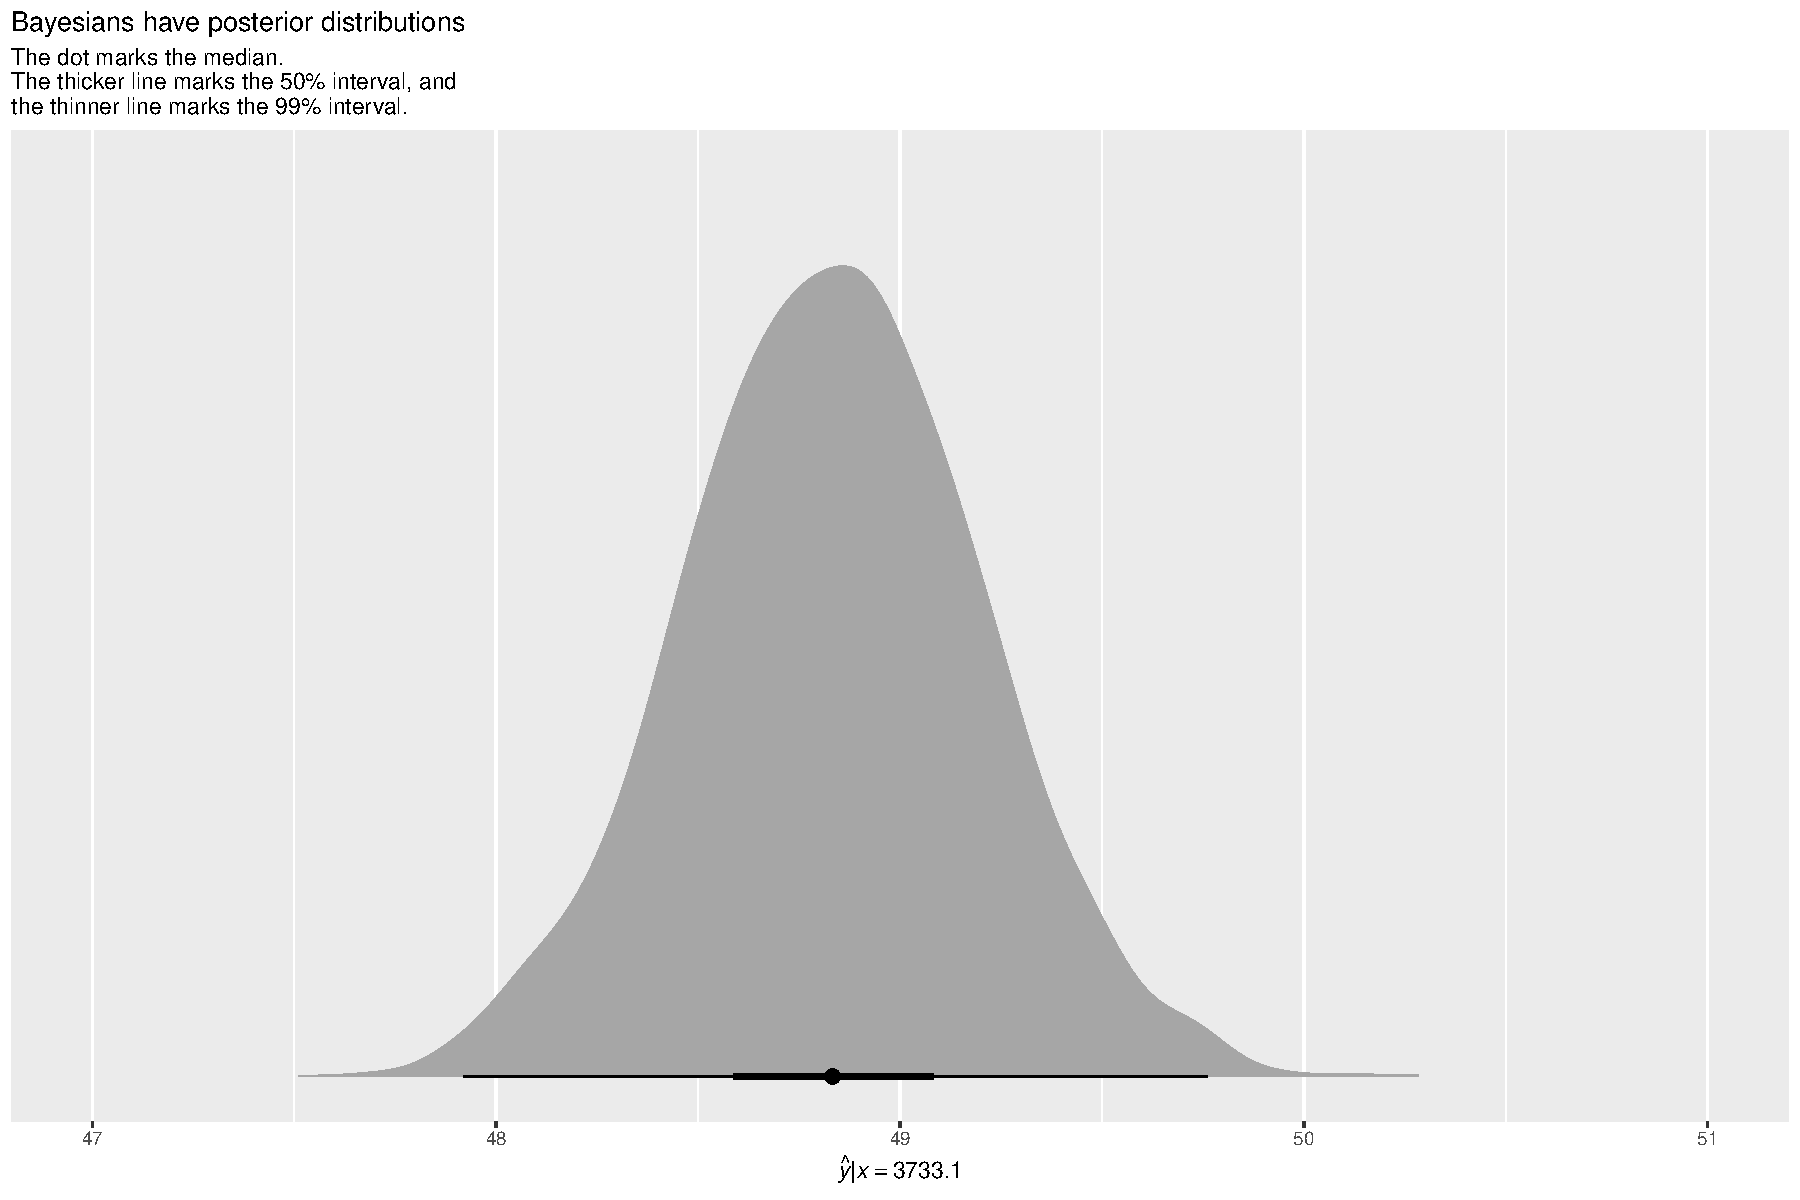
\includegraphics{Bayes_Lab_1_files/figure-pdf/unnamed-chunk-46-1.pdf}

\subsection{About those means, SD's, and
intervals.}\label{about-those-means-sds-and-intervals.}

You can describe a Bayesian posterior in a lot of different ways.
Earlier we said the posterior mean is the Bayesian point estimate. This
isn't strictly true. Means are very popular, but you can summarize a
posterior by its mean, median, or mode.

Let's see what this looks like in practice. First, we compute and save
our statistics for each of our model parameters.

\begin{Shaded}
\begin{Highlighting}[]
\NormalTok{points }\OtherTok{\textless{}{-}}\NormalTok{ draws }\SpecialCharTok{\%\textgreater{}\%} 
  \FunctionTok{rename}\NormalTok{(}\StringTok{\textasciigrave{}}\AttributeTok{beta[0]}\StringTok{\textasciigrave{}} \OtherTok{=}\NormalTok{ beta0,}
         \StringTok{\textasciigrave{}}\AttributeTok{beta[1]}\StringTok{\textasciigrave{}} \OtherTok{=}\NormalTok{ beta1) }\SpecialCharTok{\%\textgreater{}\%} 
  \FunctionTok{pivot\_longer}\NormalTok{(}\AttributeTok{cols =} \FunctionTok{c}\NormalTok{(}\StringTok{\textasciigrave{}}\AttributeTok{beta[0]}\StringTok{\textasciigrave{}}\NormalTok{, }\StringTok{\textasciigrave{}}\AttributeTok{beta[1]}\StringTok{\textasciigrave{}}\NormalTok{, sigma), }
               \AttributeTok{names\_to =} \StringTok{"parameter"}\NormalTok{) }\SpecialCharTok{\%\textgreater{}\%} 
  \FunctionTok{group\_by}\NormalTok{(parameter) }\SpecialCharTok{\%\textgreater{}\%} 
  \FunctionTok{summarise}\NormalTok{(}\AttributeTok{mean =} \FunctionTok{mean}\NormalTok{(value),}
            \AttributeTok{median =} \FunctionTok{median}\NormalTok{(value),}
            \AttributeTok{mode =} \FunctionTok{Mode}\NormalTok{(value)) }\SpecialCharTok{\%\textgreater{}\%} 
  \FunctionTok{pivot\_longer}\NormalTok{(}\FunctionTok{starts\_with}\NormalTok{(}\StringTok{"m"}\NormalTok{), }\AttributeTok{names\_to =} \StringTok{"statistic"}\NormalTok{)}

\CommentTok{\# what?}
\NormalTok{points}
\end{Highlighting}
\end{Shaded}

\begin{verbatim}
# A tibble: 9 x 3
  parameter statistic    value
  <chr>     <chr>        <dbl>
1 beta[0]   mean      32.1    
2 beta[0]   median    32.1    
3 beta[0]   mode      32.3    
4 beta[1]   mean       0.00447
5 beta[1]   median     0.00446
6 beta[1]   mode       0.00441
7 sigma     mean       2.92   
8 sigma     median     2.90   
9 sigma     mode       2.83   
\end{verbatim}

Now plot.

\begin{Shaded}
\begin{Highlighting}[]
\NormalTok{draws }\SpecialCharTok{\%\textgreater{}\%} 
  \FunctionTok{rename}\NormalTok{(}\StringTok{\textasciigrave{}}\AttributeTok{beta[0]}\StringTok{\textasciigrave{}} \OtherTok{=}\NormalTok{ beta0,}
         \StringTok{\textasciigrave{}}\AttributeTok{beta[1]}\StringTok{\textasciigrave{}} \OtherTok{=}\NormalTok{ beta1) }\SpecialCharTok{\%\textgreater{}\%} 
  \FunctionTok{pivot\_longer}\NormalTok{(}\AttributeTok{cols =} \FunctionTok{c}\NormalTok{(}\StringTok{\textasciigrave{}}\AttributeTok{beta[0]}\StringTok{\textasciigrave{}}\NormalTok{, }\StringTok{\textasciigrave{}}\AttributeTok{beta[1]}\StringTok{\textasciigrave{}}\NormalTok{, sigma), }
               \AttributeTok{names\_to =} \StringTok{"parameter"}\NormalTok{) }\SpecialCharTok{\%\textgreater{}\%} 
  
  \FunctionTok{ggplot}\NormalTok{(}\FunctionTok{aes}\NormalTok{(}\AttributeTok{x =}\NormalTok{ value)) }\SpecialCharTok{+}
  \FunctionTok{geom\_density}\NormalTok{() }\SpecialCharTok{+}
  \FunctionTok{geom\_vline}\NormalTok{(}\AttributeTok{data =}\NormalTok{ points,}
             \FunctionTok{aes}\NormalTok{(}\AttributeTok{xintercept =}\NormalTok{ value, }\AttributeTok{color =}\NormalTok{ statistic),}
             \AttributeTok{size =} \DecValTok{3}\SpecialCharTok{/}\DecValTok{4}\NormalTok{) }\SpecialCharTok{+}
  \FunctionTok{scale\_color\_viridis\_d}\NormalTok{(}\AttributeTok{option =} \StringTok{"A"}\NormalTok{, }\AttributeTok{end =}\NormalTok{ .}\DecValTok{8}\NormalTok{) }\SpecialCharTok{+}
  \FunctionTok{scale\_y\_continuous}\NormalTok{(}\ConstantTok{NULL}\NormalTok{, }\AttributeTok{breaks =} \ConstantTok{NULL}\NormalTok{) }\SpecialCharTok{+}
  \FunctionTok{xlab}\NormalTok{(}\StringTok{"parameter space"}\NormalTok{) }\SpecialCharTok{+}
  \FunctionTok{facet\_wrap}\NormalTok{(}\SpecialCharTok{\textasciitilde{}}\NormalTok{ parameter, }\AttributeTok{labeller =}\NormalTok{ label\_parsed, }\AttributeTok{scales =} \StringTok{"free"}\NormalTok{, }\AttributeTok{ncol =} \DecValTok{1}\NormalTok{) }\SpecialCharTok{+}
  \FunctionTok{theme}\NormalTok{(}\AttributeTok{strip.text =} \FunctionTok{element\_text}\NormalTok{(}\AttributeTok{size =} \DecValTok{14}\NormalTok{))}
\end{Highlighting}
\end{Shaded}

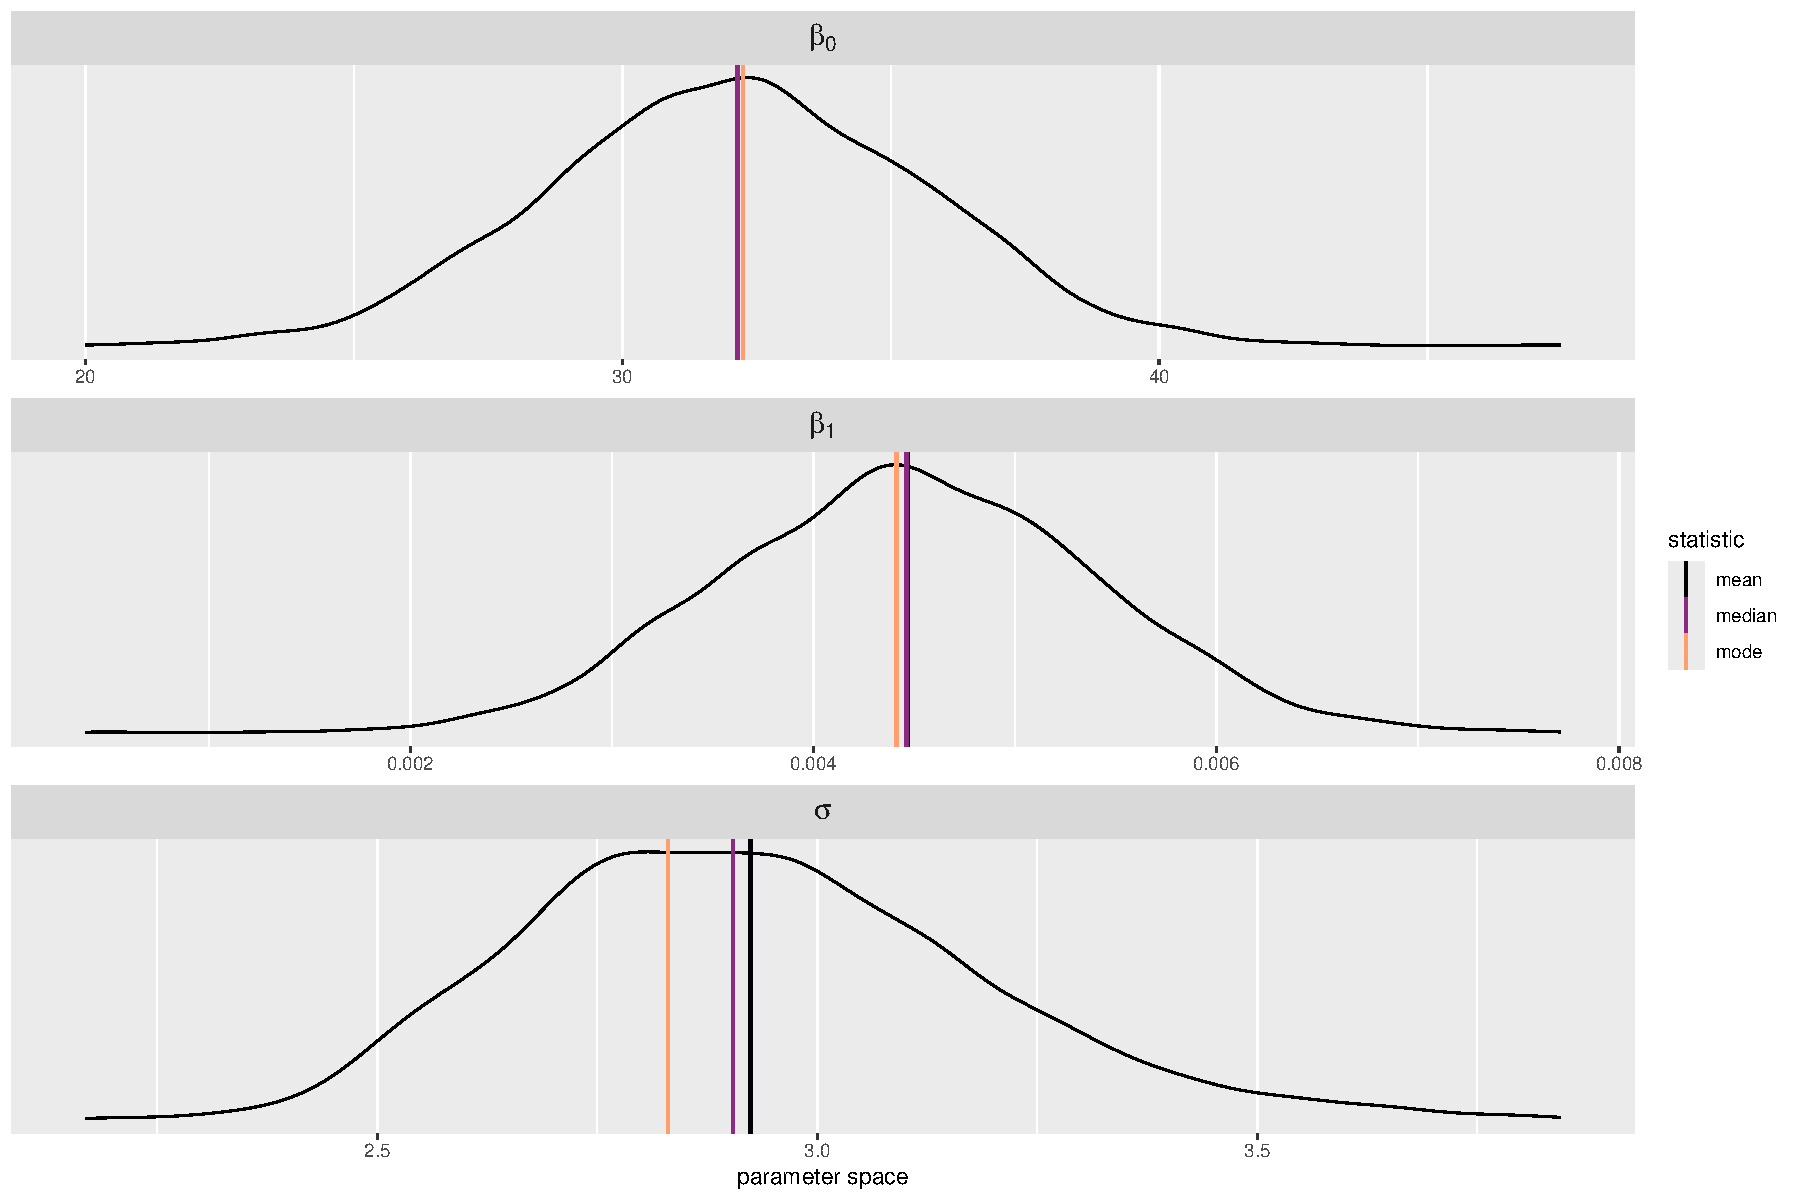
\includegraphics{Bayes_Lab_1_files/figure-pdf/unnamed-chunk-48-1.pdf}

\subsubsection{\texorpdfstring{Question 2.3: Discuss the skew in
\(\sigma\).Why it might arise,
etc.?}{Question 2.3: Discuss the skew in \textbackslash sigma.Why it might arise, etc.?}}\label{question-2.3-discuss-the-skew-in-sigma.why-it-might-arise-etc.}

\begin{verbatim}
$\sigma$ might be skewed becasue a few reasons.

First, it can't be negative, so it is bounded below 0.

Second, we might have a weak prior for $\sigma$, which will result in posterior uncertainty that includes the possibility of high residual variability, resulting in a longer right tail in the posterior.

Third, there could be some outliers that inflates $\sigma$, making its posterior distribution more right-skewed.
\end{verbatim}

\begin{itemize}
\tightlist
\item
  The mean is the \textbf{brms} default summary, and McElreath (2015,
  2020) defaulted to the mean in his texts.
\item
  The median is also available for many \textbf{brms} functions, and
  it's what Gelman et al (2020) recommend.
\item
  The mode can be attractive for very skewed distributions, and it's
  what Kruschke (2015) used in his text.
\end{itemize}

With many \textbf{brms} functions, you can request the median by setting
\texttt{robust\ =\ TRUE}. For example:

\begin{Shaded}
\begin{Highlighting}[]
\FunctionTok{fixef}\NormalTok{(fit1.b)                 }\CommentTok{\# means}
\end{Highlighting}
\end{Shaded}

\begin{verbatim}
                Estimate    Est.Error         Q2.5        Q97.5
Intercept   32.139661018 3.4974943137 25.449370922 38.886468789
body_mass_g  0.004471587 0.0009315803  0.002675154  0.006246179
\end{verbatim}

\begin{Shaded}
\begin{Highlighting}[]
\FunctionTok{fixef}\NormalTok{(fit1.b, }\AttributeTok{robust =} \ConstantTok{TRUE}\NormalTok{)  }\CommentTok{\# medians}
\end{Highlighting}
\end{Shaded}

\begin{verbatim}
                Estimate    Est.Error         Q2.5        Q97.5
Intercept   32.146445975 3.5193252356 25.449370922 38.886468789
body_mass_g  0.004462795 0.0009301993  0.002675154  0.006246179
\end{verbatim}

\subsubsection{Question 2.4: Given the skew in sigma and what you know
about summary statistics, what might be the implication of using just
the mean, median, or mode of posteriors to make a
prediction?}\label{question-2.4-given-the-skew-in-sigma-and-what-you-know-about-summary-statistics-what-might-be-the-implication-of-using-just-the-mean-median-or-mode-of-posteriors-to-make-a-prediction}

\begin{verbatim}
The mean is pulled toward the tail, so using the mean of sigma will lead to wider predicted intervals (more conservative), but we might overestimate uncertainty in new predictions if the skew is strong.

The median is robust to the skew, so using the median provides a balanced summary that is not too influenced by tail values.

The mode is often below the mean when the distribution is right skewed, so using the mode of sigma could underestimate uncertainty and produce overconfident predictions.

Overall, it is better to use the entire posterior, which full captures the uncertainty, including the skew, instead of using only a single value of the distribution.
\end{verbatim}

\paragraph{SD's and MAD SD's.}\label{sds-and-mad-sds.}

Earlier we said the posterior SD is the Bayesian standard error. This
isn't strictly true. You can also use the \emph{median absolute
deviation} (MAD SD). If we let \(M\) stand for the median of some
variable \(y\), which varies across \(i\) cases, we can define the MAD
SD as

\[
\textit{MAD SD} = 1.4826 \times \operatorname{median}_{i = 1}^n |y_i - M|,
\]

where \(1.4826\) is a constant that scales the MAD SD into a
standard-deviation metric. Here's what this looks like in practice.

\begin{Shaded}
\begin{Highlighting}[]
\CommentTok{\# go through this line by line}
\NormalTok{draws }\SpecialCharTok{\%\textgreater{}\%} 
  \FunctionTok{select}\NormalTok{(beta0) }\SpecialCharTok{\%\textgreater{}\%} 
  \FunctionTok{mutate}\NormalTok{(}\AttributeTok{mdn =} \FunctionTok{median}\NormalTok{(beta0)) }\SpecialCharTok{\%\textgreater{}\%} 
  \FunctionTok{mutate}\NormalTok{(}\StringTok{\textasciigrave{}}\AttributeTok{|yi {-} mdn|}\StringTok{\textasciigrave{}} \OtherTok{=} \FunctionTok{abs}\NormalTok{(beta0 }\SpecialCharTok{{-}}\NormalTok{ mdn)) }\SpecialCharTok{\%\textgreater{}\%} 
  \FunctionTok{summarise}\NormalTok{(}\AttributeTok{MAD\_SD =} \FloatTok{1.4826} \SpecialCharTok{*} \FunctionTok{median}\NormalTok{(}\StringTok{\textasciigrave{}}\AttributeTok{|yi {-} mdn|}\StringTok{\textasciigrave{}}\NormalTok{))}
\end{Highlighting}
\end{Shaded}

\begin{verbatim}
# A tibble: 1 x 1
  MAD_SD
   <dbl>
1   3.52
\end{verbatim}

Base \textbf{R} also has a \texttt{mad()} function.

\begin{Shaded}
\begin{Highlighting}[]
\NormalTok{?mad}
\end{Highlighting}
\end{Shaded}

\begin{verbatim}
Help on topic 'mad' was found in the following packages:

  Package               Library
  posterior             /Users/kw1166/Library/Caches/org.R-project.R/R/renv/cache/v5/macos/R-4.4/x86_64-apple-darwin20/posterior/1.6.0/fc1213566f2ed9f0b15bef656ed1000b
  stats                 /Library/Frameworks/R.framework/Versions/4.4-x86_64/Resources/library


Using the first match ...
\end{verbatim}

\begin{Shaded}
\begin{Highlighting}[]
\NormalTok{draws }\SpecialCharTok{\%\textgreater{}\%} 
  \FunctionTok{summarise}\NormalTok{(}\AttributeTok{MAD\_SD =} \FunctionTok{mad}\NormalTok{(beta0))}
\end{Highlighting}
\end{Shaded}

\begin{verbatim}
# A tibble: 1 x 1
  MAD_SD
   <dbl>
1   3.52
\end{verbatim}

You can request the MAD SD from many \textbf{brms} functions by setting
\texttt{robust\ =\ TRUE}.

\begin{Shaded}
\begin{Highlighting}[]
\FunctionTok{fixef}\NormalTok{(fit1.b)                 }\CommentTok{\# SD}
\end{Highlighting}
\end{Shaded}

\begin{verbatim}
                Estimate    Est.Error         Q2.5        Q97.5
Intercept   32.139661018 3.4974943137 25.449370922 38.886468789
body_mass_g  0.004471587 0.0009315803  0.002675154  0.006246179
\end{verbatim}

\begin{Shaded}
\begin{Highlighting}[]
\FunctionTok{fixef}\NormalTok{(fit1.b, }\AttributeTok{robust =} \ConstantTok{TRUE}\NormalTok{)  }\CommentTok{\# MAD SD}
\end{Highlighting}
\end{Shaded}

\begin{verbatim}
                Estimate    Est.Error         Q2.5        Q97.5
Intercept   32.146445975 3.5193252356 25.449370922 38.886468789
body_mass_g  0.004462795 0.0009301993  0.002675154  0.006246179
\end{verbatim}

\begin{itemize}
\tightlist
\item
  To my eye, many authors (e.g., Kruschke, McElreath) just use the SD.
\item
  Gelman et al (see Section 5.3) recommend the MAD SD.
\end{itemize}

\paragraph{Bayesian intervals.}\label{bayesian-intervals.}

Bayesians describe the widths of their posteriors with intervals. I've
seen these variously described as confidence intervals, credible
intervals, probability intervals, and even uncertainty intervals. My
recommendation is just pick a term, and clearly tell your audience what
you mean (e.g., at the end of a Method section in a journal article).

To my eye, the most popular interval is a 95\% percentile-based
interval. 95\% is conventional, perhaps due to the popularity of the
95\% frequentist confidence interval, which is related to the 0.05 alpha
level used for the conventional \(p\)-value cutoff. However, you can use
other percentiles. Some common alternatives are 99\%, 89\%, 80\%, and
50\%.

Also, Bayesian intervals aren't always percentile based. An alternative
is the highest posterior density interval (HPDI), which has mathematical
properties some find desirable.

\textbf{brms} only supports percentile-based intervals, but it does
allow for a variety of different ranges via the \texttt{prob} argument.
For example, here's how to request 80\% intervals in \texttt{summary()}.

\begin{Shaded}
\begin{Highlighting}[]
\FunctionTok{summary}\NormalTok{(fit1.b, }\AttributeTok{prob =}\NormalTok{ .}\DecValTok{80}\NormalTok{)}
\end{Highlighting}
\end{Shaded}

\begin{verbatim}
 Family: gaussian 
  Links: mu = identity; sigma = identity 
Formula: bill_length_mm ~ 1 + body_mass_g 
   Data: chinstrap (Number of observations: 68) 
  Draws: 4 chains, each with iter = 2000; warmup = 1000; thin = 1;
         total post-warmup draws = 4000

Regression Coefficients:
            Estimate Est.Error l-80% CI u-80% CI Rhat Bulk_ESS Tail_ESS
Intercept      32.14      3.50    27.61    36.64 1.00     4820     2982
body_mass_g     0.00      0.00     0.00     0.01 1.00     4861     3170

Further Distributional Parameters:
      Estimate Est.Error l-80% CI u-80% CI Rhat Bulk_ESS Tail_ESS
sigma     2.92      0.26     2.60     3.26 1.00     2015     1688

Draws were sampled using sampling(NUTS). For each parameter, Bulk_ESS
and Tail_ESS are effective sample size measures, and Rhat is the potential
scale reduction factor on split chains (at convergence, Rhat = 1).
\end{verbatim}

Regarding interval widths:

\begin{itemize}
\tightlist
\item
  95\% Intervals are widely used.
\item
  McElreat likes 89\% intervals, and uses them as a default in his
  \textbf{rethinking} package.
\item
  Some of the \textbf{bayesplot}, \textbf{ggdist}, and
  \textbf{tidybayes} functions return 80\% intervals.
\item
  Some of the \textbf{ggdist}, and \textbf{tidybayes} functions return
  66\% or 50\% intervals.
\item
  I've heard Gelman report his fondness for 50\% intervals on his blog
  (https://statmodeling.stat.columbia.edu/2016/11/05/why-i-prefer-50-to-95-intervals/).
\end{itemize}

Regarding interval types:

\begin{itemize}
\tightlist
\item
  Percentile-based intervals are widely used in the Stan ecosystem, and
  are supported in texts like Gelman et al.
\item
  Kruschke has consistently advocates for HPDI's in his articles, and in
  his text.
\end{itemize}

\subsubsection{\texorpdfstring{Posterior summaries with
\textbf{tidybayes}.}{Posterior summaries with tidybayes.}}\label{posterior-summaries-with-tidybayes.}

Matthew Kay's \textbf{tidybayes} package
(https://mjskay.github.io/tidybayes/) offers an array of convenience
functions for summarizing posterior distributions with points and
intervals. See the \emph{Point summaries and intervals} section of Kay's
\emph{Extracting and visualizing tidy draws from brms models} vignette
(https://mjskay.github.io/tidybayes/articles/tidy-brms.html\#point-summaries-and-intervals)
for a detailed breakdown. In short, the family of functions use the
naming scheme
\texttt{{[}median\textbar{}mean\textbar{}mode{]}\_{[}qi\textbar{}hdi{]}}.
Here are a few examples.

\begin{Shaded}
\begin{Highlighting}[]
\NormalTok{draws }\SpecialCharTok{\%\textgreater{}\%} \FunctionTok{mean\_qi}\NormalTok{(beta0)                        }\CommentTok{\# mean and 95\% percentile interval}
\end{Highlighting}
\end{Shaded}

\begin{verbatim}
# A tibble: 1 x 6
  beta0 .lower .upper .width .point .interval
  <dbl>  <dbl>  <dbl>  <dbl> <chr>  <chr>    
1  32.1   25.4   38.9   0.95 mean   qi       
\end{verbatim}

\begin{Shaded}
\begin{Highlighting}[]
\NormalTok{draws }\SpecialCharTok{\%\textgreater{}\%} \FunctionTok{median\_qi}\NormalTok{(beta0, }\AttributeTok{.width =}\NormalTok{ .}\DecValTok{80}\NormalTok{)        }\CommentTok{\# median and 80\% percentile interval}
\end{Highlighting}
\end{Shaded}

\begin{verbatim}
# A tibble: 1 x 6
  beta0 .lower .upper .width .point .interval
  <dbl>  <dbl>  <dbl>  <dbl> <chr>  <chr>    
1  32.1   27.6   36.6    0.8 median qi       
\end{verbatim}

\begin{Shaded}
\begin{Highlighting}[]
\NormalTok{draws }\SpecialCharTok{\%\textgreater{}\%} \FunctionTok{mode\_hdi}\NormalTok{(beta0, }\AttributeTok{.width =} \FunctionTok{c}\NormalTok{(.}\DecValTok{5}\NormalTok{, .}\DecValTok{95}\NormalTok{))  }\CommentTok{\# mode, with 95 and 50\% HPDI\textquotesingle{}s}
\end{Highlighting}
\end{Shaded}

\begin{verbatim}
# A tibble: 2 x 6
  beta0 .lower .upper .width .point .interval
  <dbl>  <dbl>  <dbl>  <dbl> <chr>  <chr>    
1  32.3   29.5   34.2   0.5  mode   hdi      
2  32.3   25.4   38.8   0.95 mode   hdi      
\end{verbatim}

As an aside, the \texttt{Mode()} function we used a while back was also
from \textbf{tidybayes}.

\subsubsection{Spaghetti plots.}\label{spaghetti-plots.}

Remember how we said the \texttt{draw} was something like 4,000 separate
equations for our Bayesian model? Let's see that again.

\begin{Shaded}
\begin{Highlighting}[]
\NormalTok{draws }\SpecialCharTok{\%\textgreater{}\%} 
  \FunctionTok{select}\NormalTok{(.draw, beta0, beta1) }\SpecialCharTok{\%\textgreater{}\%} 
  \FunctionTok{mutate}\NormalTok{(}\AttributeTok{body\_mass\_g =} \FunctionTok{mean}\NormalTok{(chinstrap}\SpecialCharTok{$}\NormalTok{body\_mass\_g)) }\SpecialCharTok{\%\textgreater{}\%} 
  \CommentTok{\# here\textquotesingle{}s the equation}
  \FunctionTok{mutate}\NormalTok{(}\AttributeTok{y\_hat =}\NormalTok{ beta0 }\SpecialCharTok{+}\NormalTok{ beta1 }\SpecialCharTok{*}\NormalTok{ body\_mass\_g) }\SpecialCharTok{\%\textgreater{}\%} 
  \CommentTok{\# subset the top 6}
  \FunctionTok{head}\NormalTok{()}
\end{Highlighting}
\end{Shaded}

\begin{verbatim}
# A tibble: 6 x 5
  .draw beta0   beta1 body_mass_g y_hat
  <int> <dbl>   <dbl>       <dbl> <dbl>
1     1  32.0 0.00442       3733.  48.5
2     2  29.8 0.00500       3733.  48.5
3     3  32.8 0.00432       3733.  48.9
4     4  32.8 0.00432       3733.  48.9
5     5  31.9 0.00446       3733.  48.6
6     6  31.4 0.00465       3733.  48.8
\end{verbatim}

One way we might emphasize the 4,000 equations is with a spaghetti plot.
When we display the fitted line for \texttt{bill\_length\_mm} over the
range of \texttt{body\_mass\_g} values, we can display a single line for
each posterior draw. Here's what that can look like.

\begin{Shaded}
\begin{Highlighting}[]
\FunctionTok{range}\NormalTok{(chinstrap}\SpecialCharTok{$}\NormalTok{body\_mass\_g)}
\end{Highlighting}
\end{Shaded}

\begin{verbatim}
[1] 2700 4800
\end{verbatim}

\begin{Shaded}
\begin{Highlighting}[]
\CommentTok{\# Note: go through this one line at a time}
\NormalTok{draws }\SpecialCharTok{\%\textgreater{}\%} 
  \FunctionTok{select}\NormalTok{(.draw, beta0, beta1) }\SpecialCharTok{\%\textgreater{}\%} 
  \FunctionTok{expand\_grid}\NormalTok{(}\AttributeTok{body\_mass\_g =} \FunctionTok{range}\NormalTok{(chinstrap}\SpecialCharTok{$}\NormalTok{body\_mass\_g)) }\SpecialCharTok{\%\textgreater{}\%} 
  \FunctionTok{mutate}\NormalTok{(}\AttributeTok{y\_hat =}\NormalTok{ beta0 }\SpecialCharTok{+}\NormalTok{ beta1 }\SpecialCharTok{*}\NormalTok{ body\_mass\_g) }\SpecialCharTok{\%\textgreater{}\%} 
  
  \CommentTok{\# plot!}
  \FunctionTok{ggplot}\NormalTok{(}\FunctionTok{aes}\NormalTok{(}\AttributeTok{x =}\NormalTok{ body\_mass\_g, }\AttributeTok{y =}\NormalTok{ y\_hat, }\AttributeTok{group =}\NormalTok{ .draw)) }\SpecialCharTok{+}
  \FunctionTok{geom\_line}\NormalTok{(}\AttributeTok{linewidth =} \DecValTok{1}\SpecialCharTok{/}\DecValTok{10}\NormalTok{, }\AttributeTok{alpha =} \DecValTok{1}\SpecialCharTok{/}\DecValTok{10}\NormalTok{)}
\end{Highlighting}
\end{Shaded}

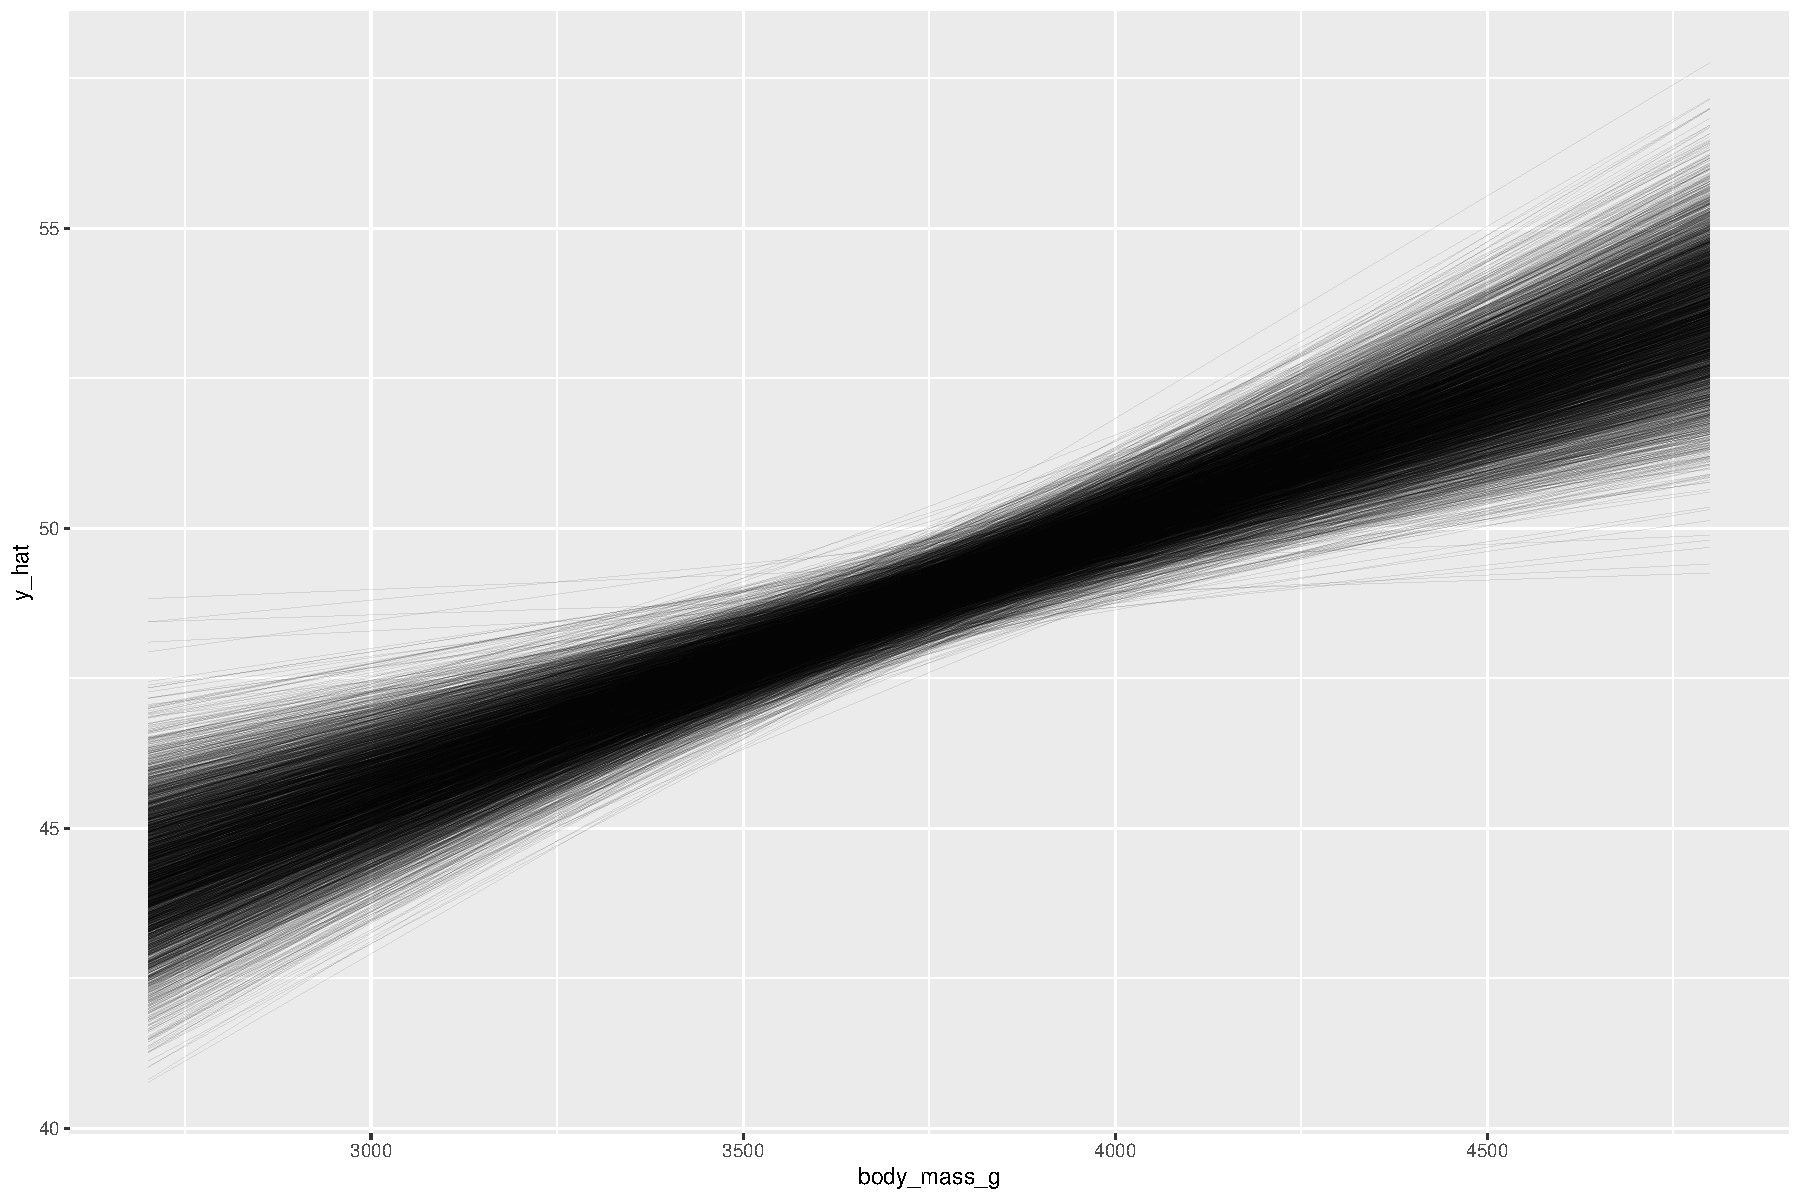
\includegraphics{Bayes_Lab_1_files/figure-pdf/unnamed-chunk-56-1.pdf}

It might be easier to see what's going on with a random subset of, say,
10 of the posterior draws.

\begin{Shaded}
\begin{Highlighting}[]
\FunctionTok{set.seed}\NormalTok{(}\DecValTok{10}\NormalTok{)}

\NormalTok{draws }\SpecialCharTok{\%\textgreater{}\%} 
  \CommentTok{\# take a random sample of 10 rows}
  \FunctionTok{slice\_sample}\NormalTok{(}\AttributeTok{n =} \DecValTok{10}\NormalTok{) }\SpecialCharTok{\%\textgreater{}\%} 
  \FunctionTok{select}\NormalTok{(.draw, beta0, beta1) }\SpecialCharTok{\%\textgreater{}\%} 
  \FunctionTok{expand\_grid}\NormalTok{(}\AttributeTok{body\_mass\_g =} \FunctionTok{range}\NormalTok{(chinstrap}\SpecialCharTok{$}\NormalTok{body\_mass\_g)) }\SpecialCharTok{\%\textgreater{}\%} 
  \FunctionTok{mutate}\NormalTok{(}\AttributeTok{y\_hat =}\NormalTok{ beta0 }\SpecialCharTok{+}\NormalTok{ beta1 }\SpecialCharTok{*}\NormalTok{ body\_mass\_g) }\SpecialCharTok{\%\textgreater{}\%} 
  
  \FunctionTok{ggplot}\NormalTok{(}\FunctionTok{aes}\NormalTok{(}\AttributeTok{x =}\NormalTok{ body\_mass\_g, }\AttributeTok{y =}\NormalTok{ y\_hat, }\AttributeTok{group =}\NormalTok{ .draw)) }\SpecialCharTok{+}
  \FunctionTok{geom\_line}\NormalTok{(}\AttributeTok{linewidth =} \DecValTok{1}\SpecialCharTok{/}\DecValTok{2}\NormalTok{, }\AttributeTok{alpha =} \DecValTok{1}\SpecialCharTok{/}\DecValTok{2}\NormalTok{)}
\end{Highlighting}
\end{Shaded}

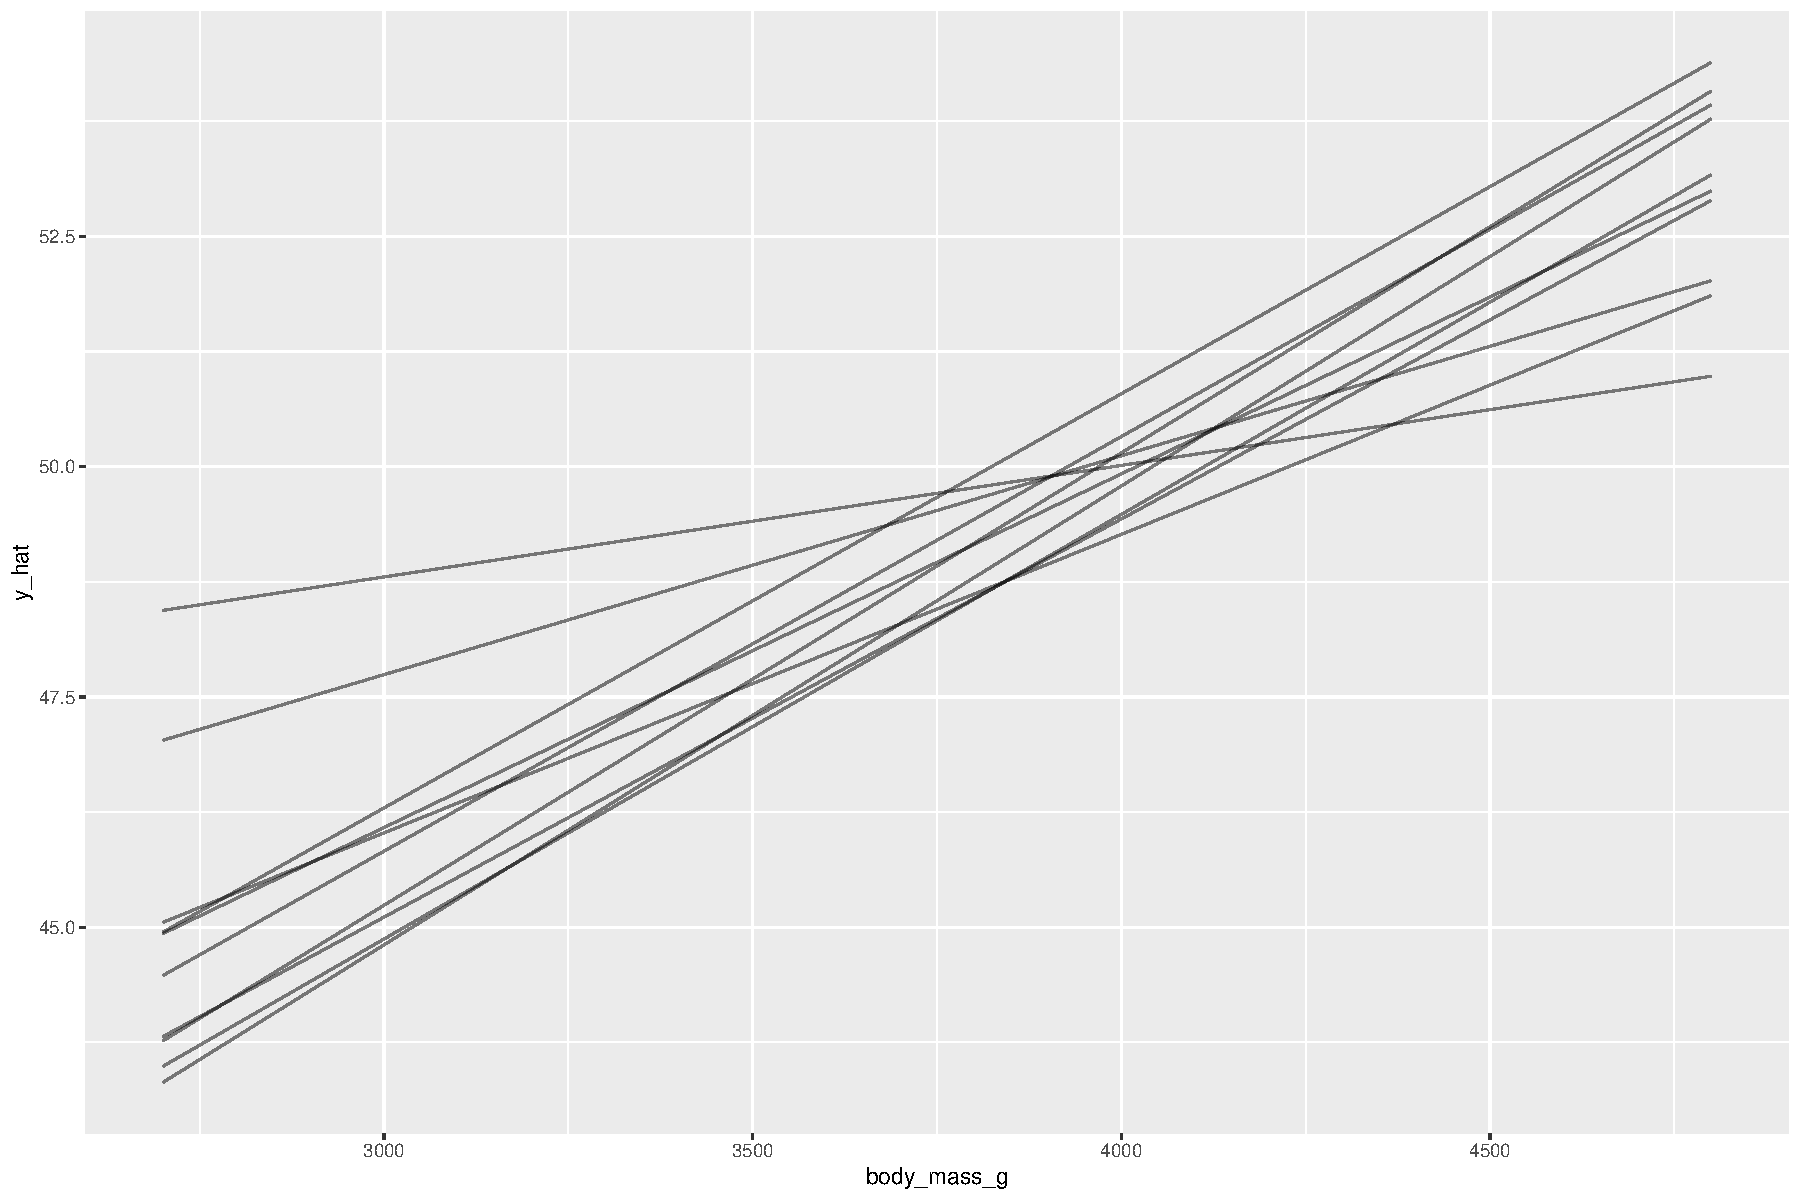
\includegraphics{Bayes_Lab_1_files/figure-pdf/unnamed-chunk-57-1.pdf}

While we're at it, let's take 20 draws and do a little color coding.

\begin{Shaded}
\begin{Highlighting}[]
\FunctionTok{set.seed}\NormalTok{(}\DecValTok{20}\NormalTok{)}

\NormalTok{draws }\SpecialCharTok{\%\textgreater{}\%} 
  \CommentTok{\# take a random sample of 20 rows}
  \FunctionTok{slice\_sample}\NormalTok{(}\AttributeTok{n =} \DecValTok{20}\NormalTok{) }\SpecialCharTok{\%\textgreater{}\%} 
  \FunctionTok{select}\NormalTok{(.draw, beta0, beta1) }\SpecialCharTok{\%\textgreater{}\%} 
  \FunctionTok{expand\_grid}\NormalTok{(}\AttributeTok{body\_mass\_g =} \FunctionTok{range}\NormalTok{(chinstrap}\SpecialCharTok{$}\NormalTok{body\_mass\_g)) }\SpecialCharTok{\%\textgreater{}\%} 
  \FunctionTok{mutate}\NormalTok{(}\AttributeTok{y\_hat =}\NormalTok{ beta0 }\SpecialCharTok{+}\NormalTok{ beta1 }\SpecialCharTok{*}\NormalTok{ body\_mass\_g) }\SpecialCharTok{\%\textgreater{}\%} 
  
  \FunctionTok{ggplot}\NormalTok{(}\FunctionTok{aes}\NormalTok{(}\AttributeTok{x =}\NormalTok{ body\_mass\_g, }\AttributeTok{y =}\NormalTok{ y\_hat, }\AttributeTok{group =}\NormalTok{ .draw, }\AttributeTok{color =}\NormalTok{ beta0)) }\SpecialCharTok{+}
  \FunctionTok{geom\_line}\NormalTok{() }\SpecialCharTok{+}
  \FunctionTok{scale\_color\_viridis\_c}\NormalTok{(}\FunctionTok{expression}\NormalTok{(beta[}\DecValTok{0}\NormalTok{]}\SpecialCharTok{\textasciitilde{}}\NormalTok{(the}\SpecialCharTok{\textasciitilde{}}\NormalTok{intercept)), }\AttributeTok{end =}\NormalTok{ .}\DecValTok{9}\NormalTok{)}
\end{Highlighting}
\end{Shaded}

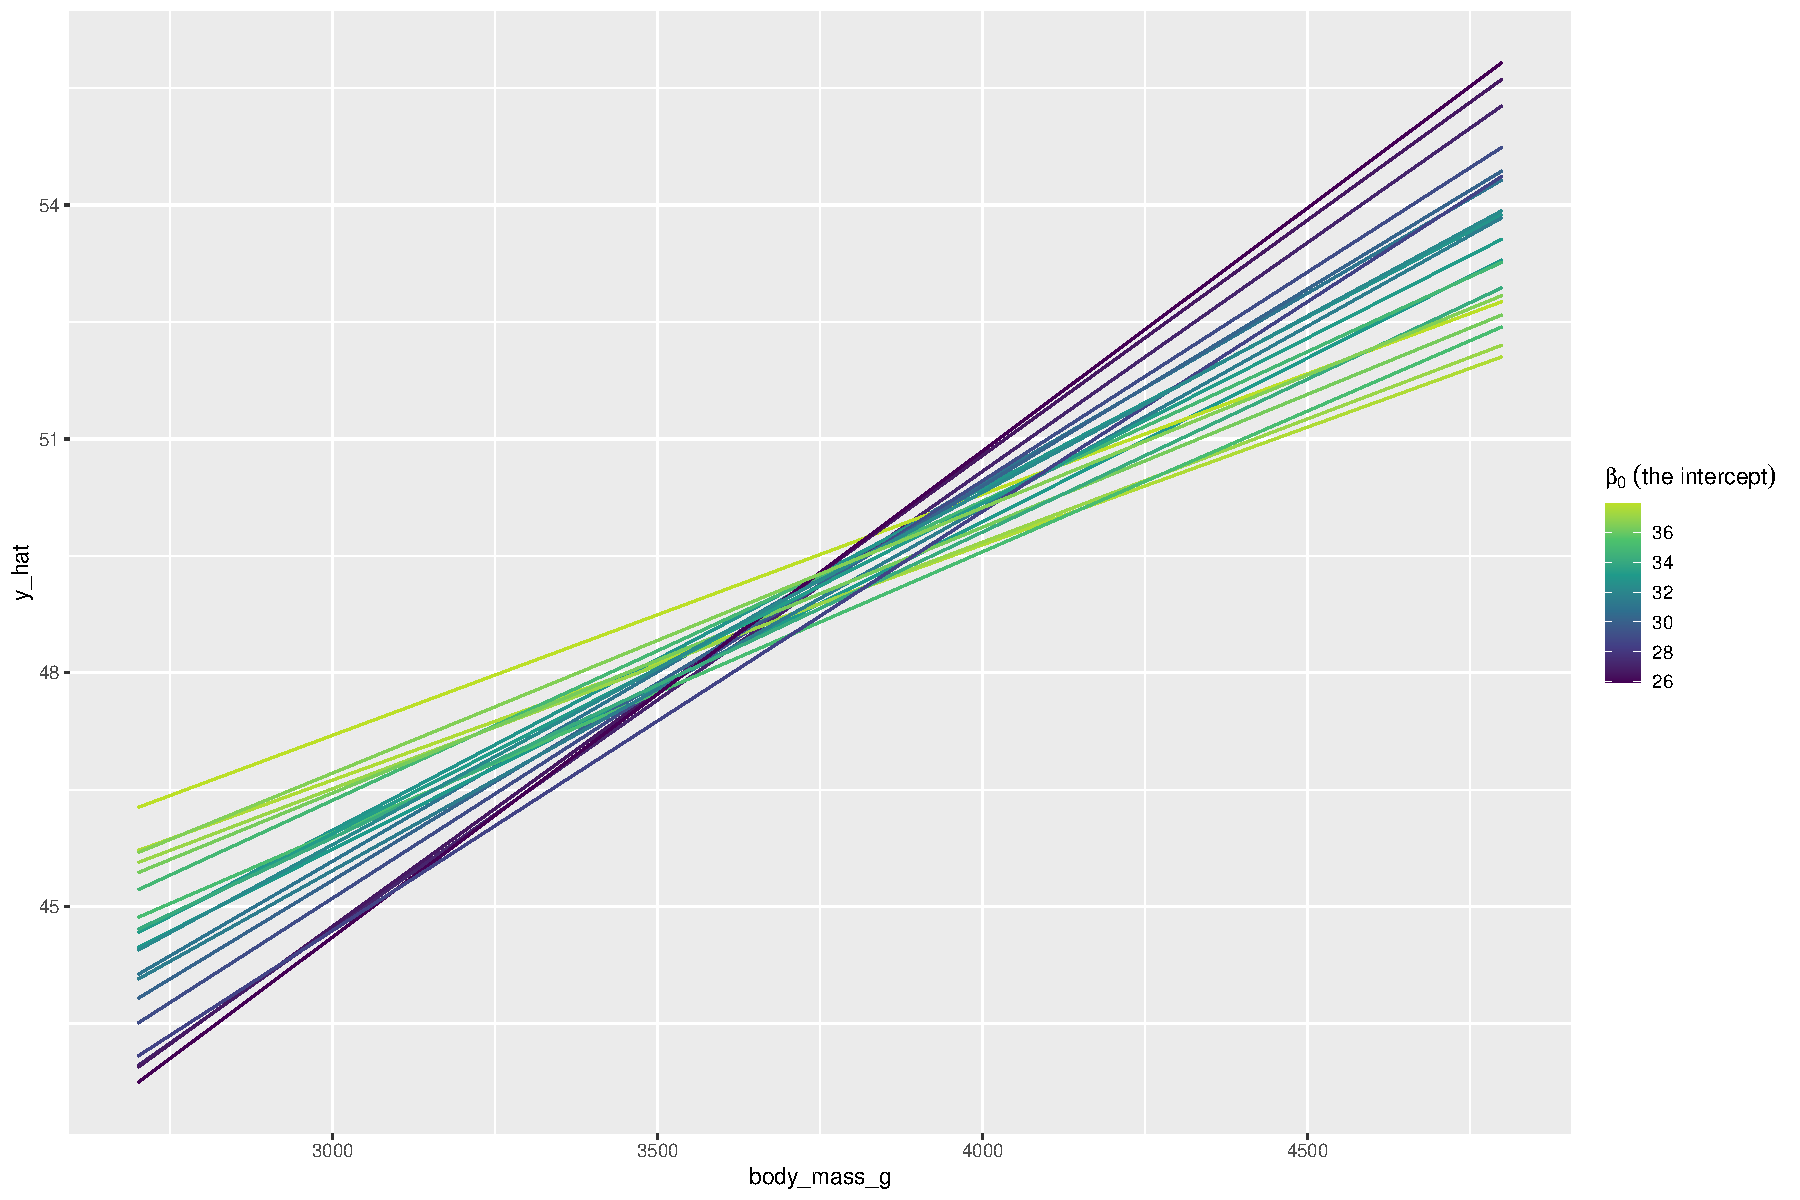
\includegraphics{Bayes_Lab_1_files/figure-pdf/unnamed-chunk-58-1.pdf}

Do you remember how we said \(\beta_0\) and \(\beta_1\) had a strong
negative correlation? Notice how the lines computed by lower \(\beta_0\)
values also tend to have higher slopes. This will happen all the time
with conventional regression models.

\subsubsection{Question 2.5: We have done all this without yet
specifying a prior. What do you think is going
on?}\label{question-2.5-we-have-done-all-this-without-yet-specifying-a-prior.-what-do-you-think-is-going-on}

\begin{verbatim}
The brms package assigns default priors (weakly informative priors) to all the parameters, even though we didn't specify any.
\end{verbatim}

\subsection{Question/Exercise:}\label{questionexercise}

In the last part, we made a subset of the \texttt{penguins} data called
\texttt{gentoo}, which was only the cases for which
\texttt{species\ ==\ "Gentoo"}. Do that again and refit the Bayesian
model to those data. Can you then remake some of the figures in this
file with the new version of the model?

\begin{Shaded}
\begin{Highlighting}[]
\CommentTok{\# wrangle}
\FunctionTok{as\_draws\_df}\NormalTok{(fit2.b) }\SpecialCharTok{\%\textgreater{}\%} 
  \FunctionTok{pivot\_longer}\NormalTok{(}\FunctionTok{starts\_with}\NormalTok{(}\StringTok{"b\_"}\NormalTok{)) }\SpecialCharTok{\%\textgreater{}\%} 
  
  \CommentTok{\# plot!}
  \FunctionTok{ggplot}\NormalTok{(}\FunctionTok{aes}\NormalTok{(}\AttributeTok{x =}\NormalTok{ value)) }\SpecialCharTok{+} 
  \CommentTok{\# geom\_density(fill = "grey20") +}
  \FunctionTok{geom\_histogram}\NormalTok{(}\AttributeTok{bins =} \DecValTok{40}\NormalTok{) }\SpecialCharTok{+}
  \FunctionTok{facet\_wrap}\NormalTok{(}\SpecialCharTok{\textasciitilde{}}\NormalTok{ name, }\AttributeTok{scales =} \StringTok{"free"}\NormalTok{)}
\end{Highlighting}
\end{Shaded}

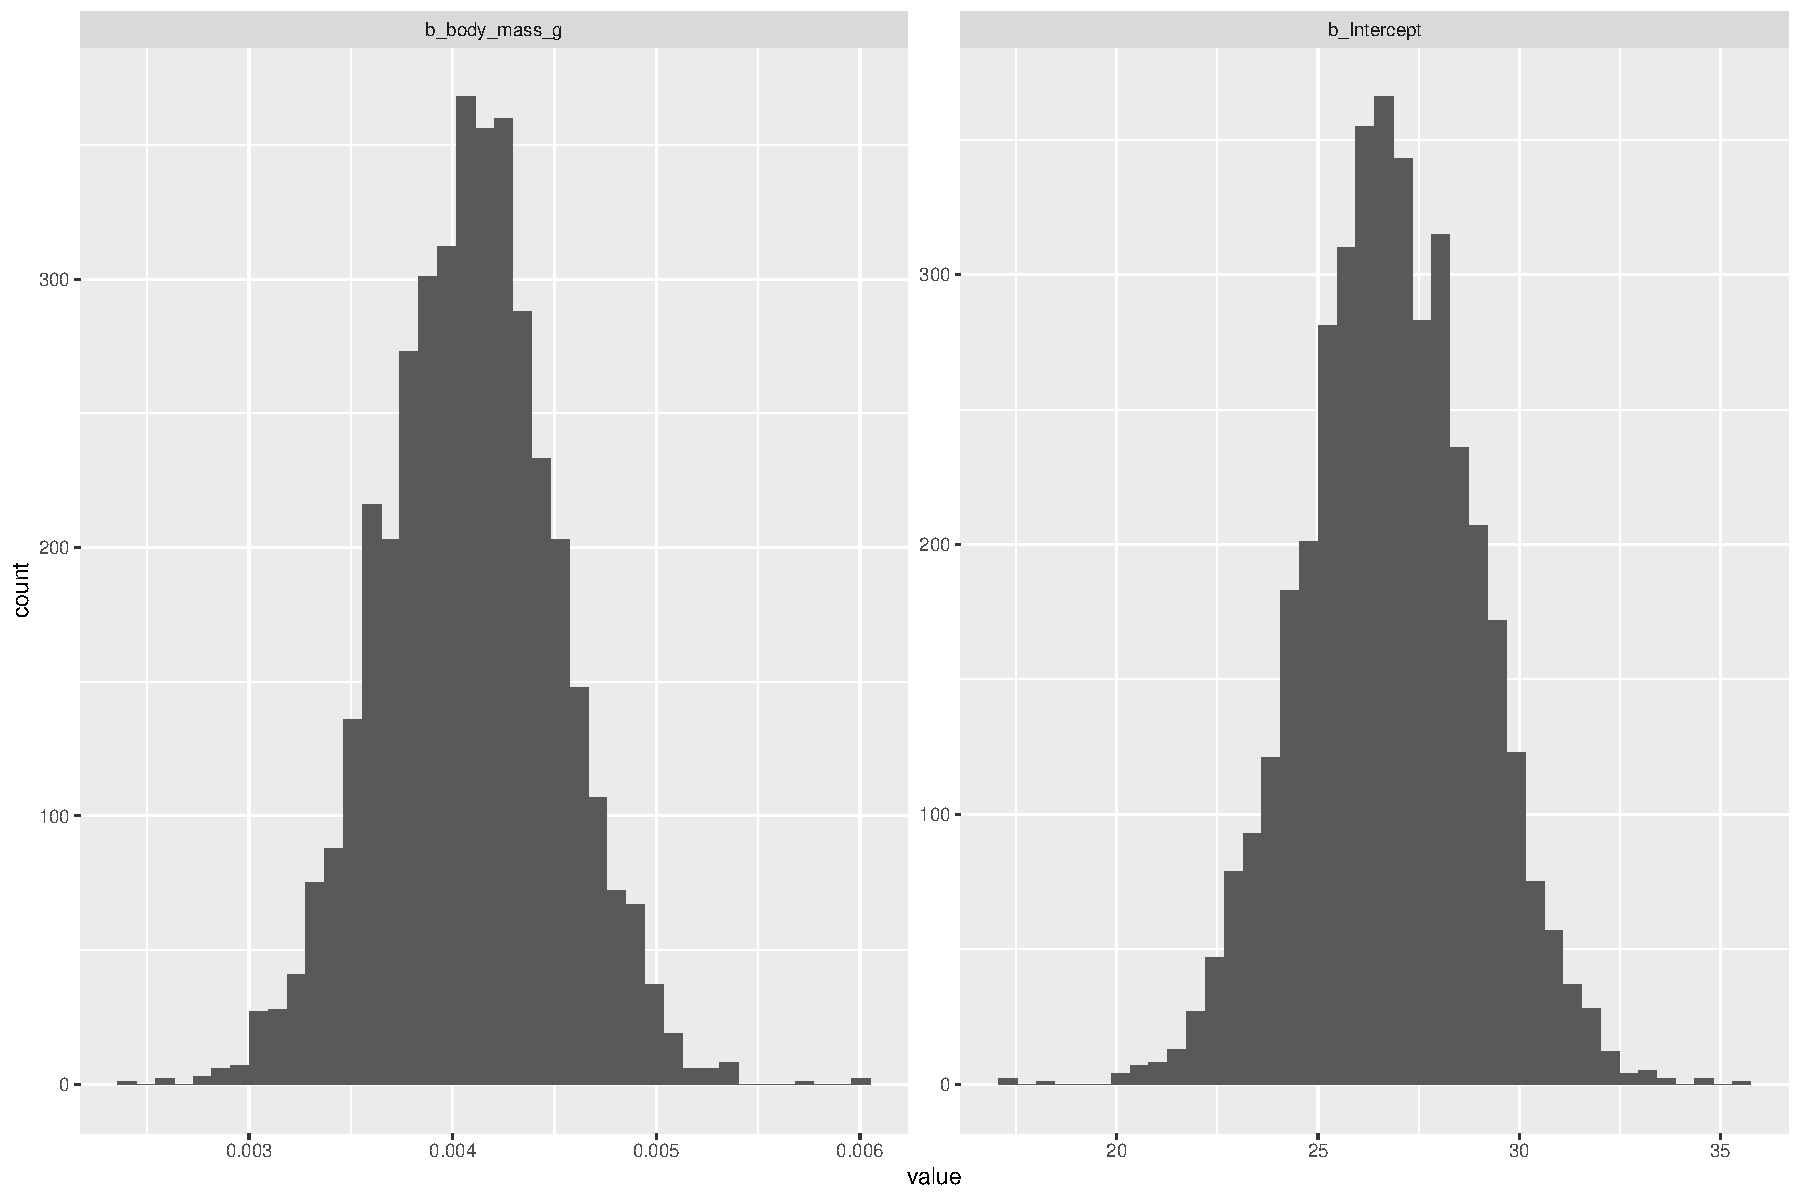
\includegraphics{Bayes_Lab_1_files/figure-pdf/unnamed-chunk-59-1.pdf}

\begin{Shaded}
\begin{Highlighting}[]
\FunctionTok{pairs}\NormalTok{(fit2.b)}
\end{Highlighting}
\end{Shaded}

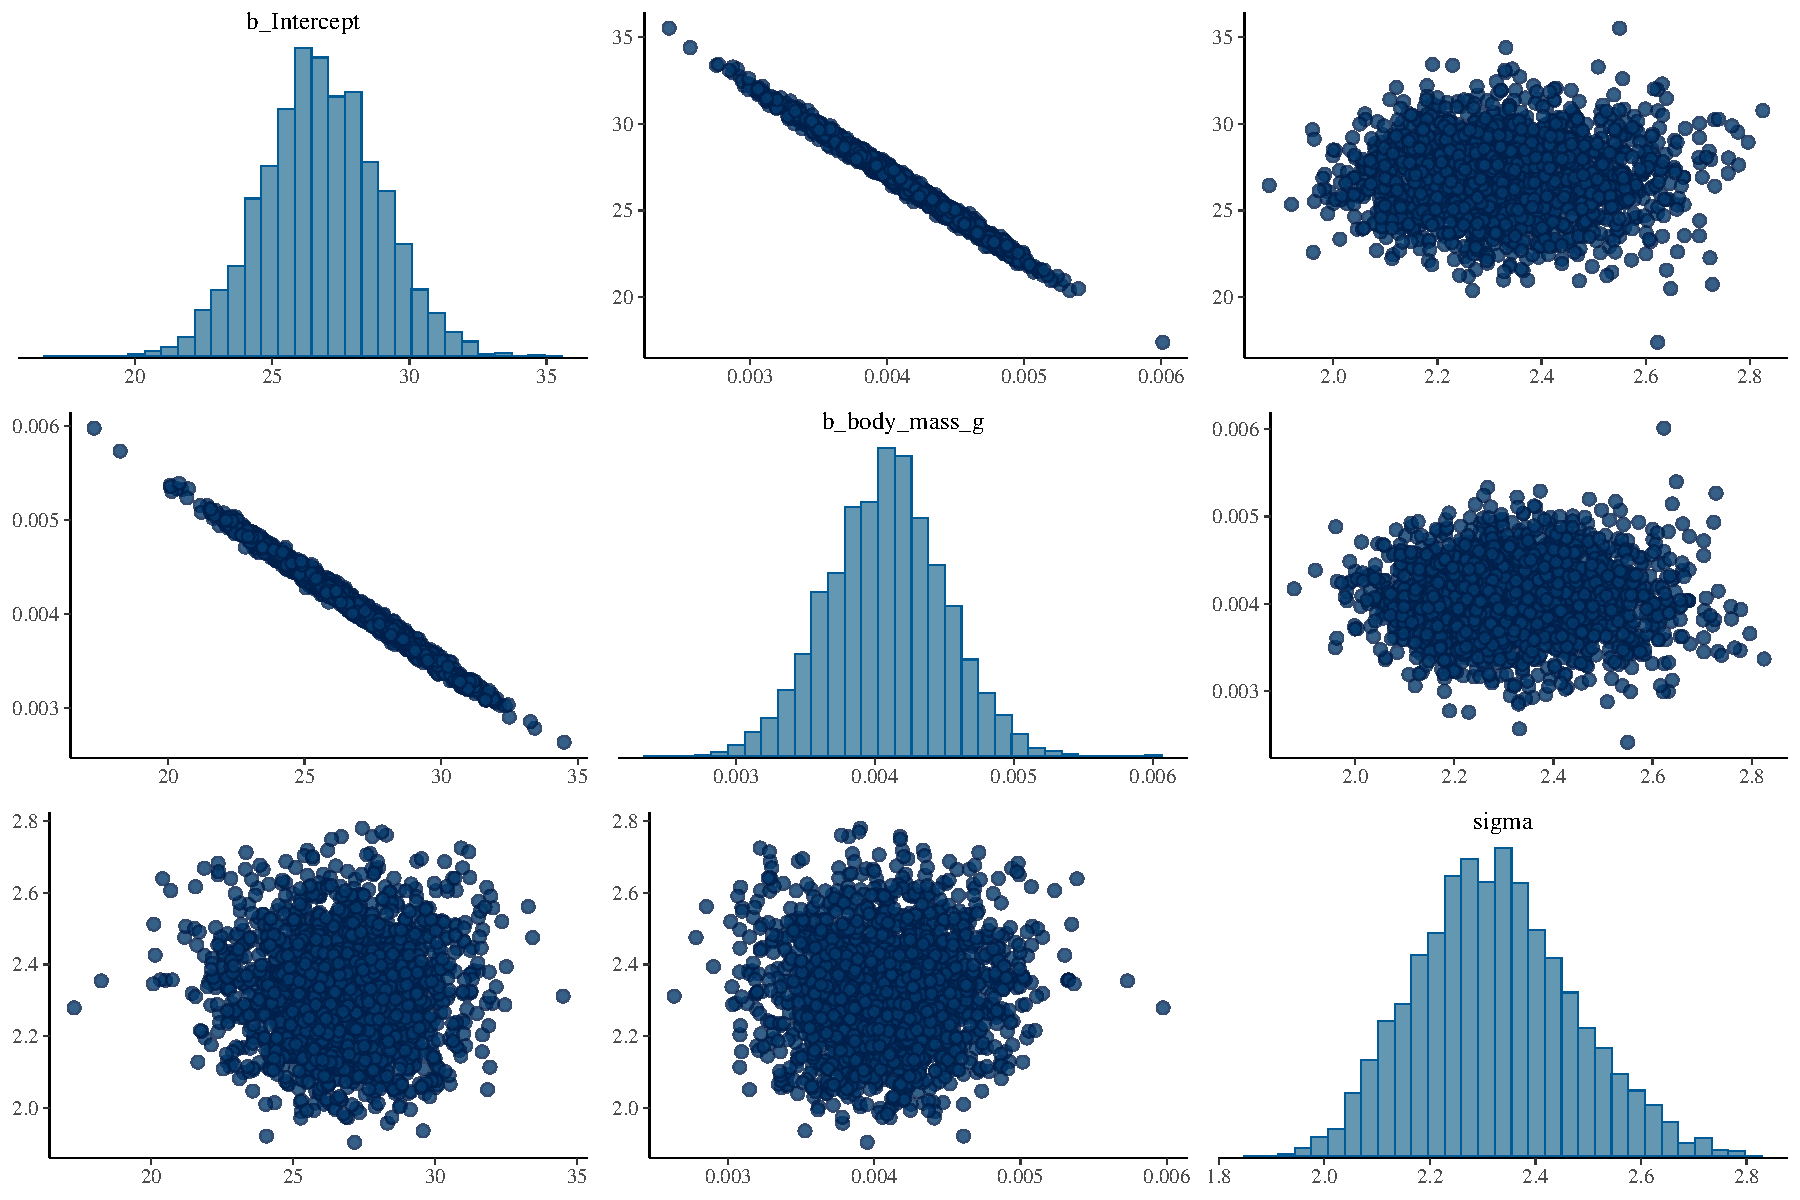
\includegraphics{Bayes_Lab_1_files/figure-pdf/unnamed-chunk-59-2.pdf}

\begin{Shaded}
\begin{Highlighting}[]
\NormalTok{draws2 }\OtherTok{\textless{}{-}} \FunctionTok{as\_draws\_df}\NormalTok{(fit2.b)}

\CommentTok{\# adjust the parameter names }
\NormalTok{draws2 }\OtherTok{\textless{}{-}}\NormalTok{ draws2 }\SpecialCharTok{\%\textgreater{}\%} 
  \FunctionTok{mutate}\NormalTok{(}\AttributeTok{beta0 =}\NormalTok{ b\_Intercept,}
         \AttributeTok{beta1 =}\NormalTok{ b\_body\_mass\_g)}

\NormalTok{draws2 }\SpecialCharTok{\%\textgreater{}\%} 
  \FunctionTok{mutate}\NormalTok{(}\AttributeTok{body\_mass\_g =} \FunctionTok{mean}\NormalTok{(gentoo}\SpecialCharTok{$}\NormalTok{body\_mass\_g, }\AttributeTok{na.rm=}\ConstantTok{TRUE}\NormalTok{)) }\SpecialCharTok{\%\textgreater{}\%} 
  \FunctionTok{mutate}\NormalTok{(}\AttributeTok{y\_hat =}\NormalTok{ beta0 }\SpecialCharTok{+}\NormalTok{ beta1 }\SpecialCharTok{*}\NormalTok{ body\_mass\_g) }\SpecialCharTok{\%\textgreater{}\%} 
  \FunctionTok{ggplot}\NormalTok{(}\FunctionTok{aes}\NormalTok{(}\AttributeTok{x =}\NormalTok{ y\_hat)) }\SpecialCharTok{+}
  \CommentTok{\# note the changes to this line}
  \FunctionTok{stat\_halfeye}\NormalTok{(}\AttributeTok{point\_interval =}\NormalTok{ median\_qi, }\AttributeTok{.width =} \FunctionTok{c}\NormalTok{(.}\DecValTok{5}\NormalTok{, .}\DecValTok{99}\NormalTok{)) }\SpecialCharTok{+}
  \FunctionTok{scale\_y\_continuous}\NormalTok{(}\ConstantTok{NULL}\NormalTok{, }\AttributeTok{breaks =} \ConstantTok{NULL}\NormalTok{) }\SpecialCharTok{+}
  \FunctionTok{labs}\NormalTok{(}\AttributeTok{title =} \StringTok{"Bayesians have posterior distributions"}\NormalTok{,}
       \AttributeTok{subtitle =} \StringTok{"The dot marks the median.}\SpecialCharTok{\textbackslash{}n}\StringTok{The thicker line marks the 50\% interval, and}\SpecialCharTok{\textbackslash{}n}\StringTok{th thinner line marks the 99\% interval."}\NormalTok{)}
\end{Highlighting}
\end{Shaded}

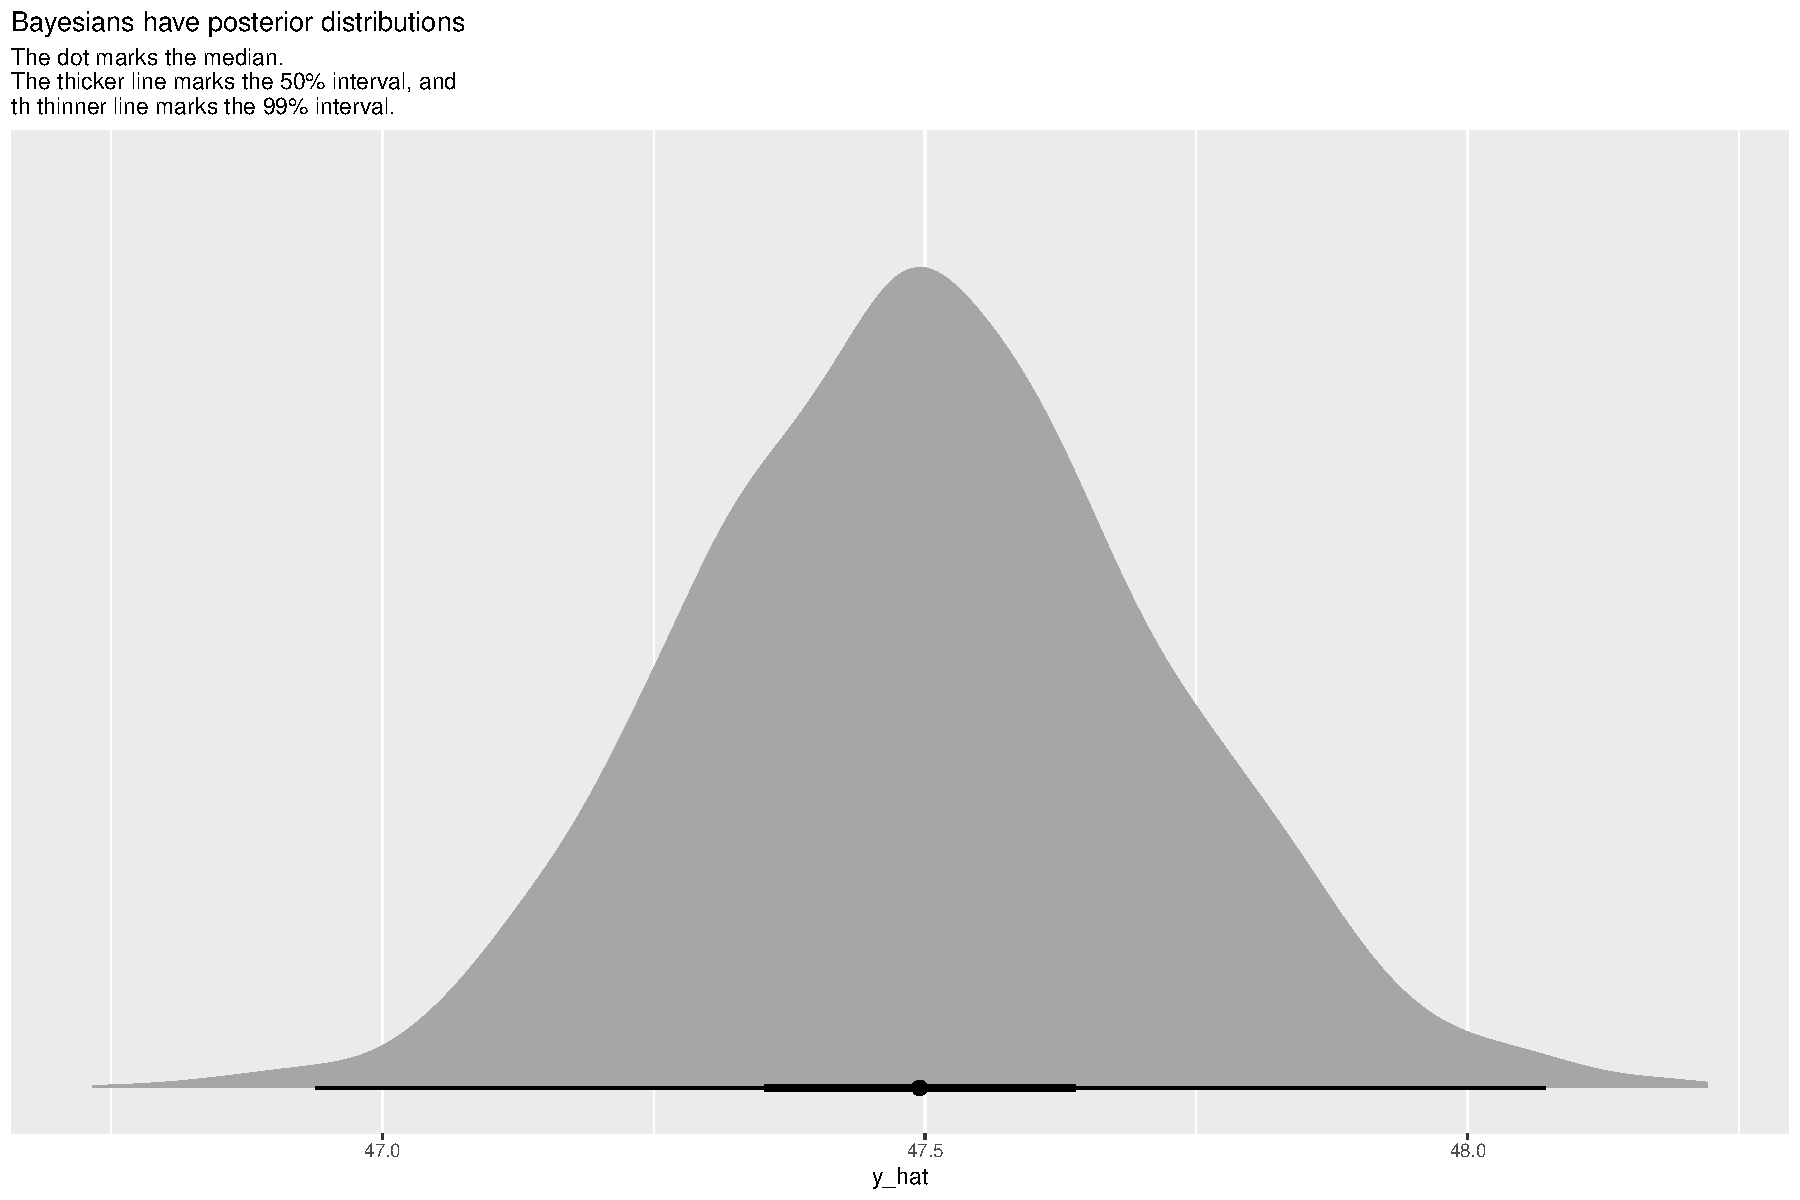
\includegraphics{Bayes_Lab_1_files/figure-pdf/unnamed-chunk-60-1.pdf}

\begin{Shaded}
\begin{Highlighting}[]
\NormalTok{points }\OtherTok{\textless{}{-}}\NormalTok{ draws2 }\SpecialCharTok{\%\textgreater{}\%} 
  \FunctionTok{rename}\NormalTok{(}\StringTok{\textasciigrave{}}\AttributeTok{beta[0]}\StringTok{\textasciigrave{}} \OtherTok{=}\NormalTok{ beta0,}
         \StringTok{\textasciigrave{}}\AttributeTok{beta[1]}\StringTok{\textasciigrave{}} \OtherTok{=}\NormalTok{ beta1) }\SpecialCharTok{\%\textgreater{}\%} 
  \FunctionTok{pivot\_longer}\NormalTok{(}\AttributeTok{cols =} \FunctionTok{c}\NormalTok{(}\StringTok{\textasciigrave{}}\AttributeTok{beta[0]}\StringTok{\textasciigrave{}}\NormalTok{, }\StringTok{\textasciigrave{}}\AttributeTok{beta[1]}\StringTok{\textasciigrave{}}\NormalTok{, sigma), }
               \AttributeTok{names\_to =} \StringTok{"parameter"}\NormalTok{) }\SpecialCharTok{\%\textgreater{}\%} 
  \FunctionTok{group\_by}\NormalTok{(parameter) }\SpecialCharTok{\%\textgreater{}\%} 
  \FunctionTok{summarise}\NormalTok{(}\AttributeTok{mean =} \FunctionTok{mean}\NormalTok{(value),}
            \AttributeTok{median =} \FunctionTok{median}\NormalTok{(value),}
            \AttributeTok{mode =} \FunctionTok{Mode}\NormalTok{(value)) }\SpecialCharTok{\%\textgreater{}\%} 
  \FunctionTok{pivot\_longer}\NormalTok{(}\FunctionTok{starts\_with}\NormalTok{(}\StringTok{"m"}\NormalTok{), }\AttributeTok{names\_to =} \StringTok{"statistic"}\NormalTok{)}


\NormalTok{draws2 }\SpecialCharTok{\%\textgreater{}\%} 
  \FunctionTok{rename}\NormalTok{(}\StringTok{\textasciigrave{}}\AttributeTok{beta[0]}\StringTok{\textasciigrave{}} \OtherTok{=}\NormalTok{ beta0,}
         \StringTok{\textasciigrave{}}\AttributeTok{beta[1]}\StringTok{\textasciigrave{}} \OtherTok{=}\NormalTok{ beta1) }\SpecialCharTok{\%\textgreater{}\%} 
  \FunctionTok{pivot\_longer}\NormalTok{(}\AttributeTok{cols =} \FunctionTok{c}\NormalTok{(}\StringTok{\textasciigrave{}}\AttributeTok{beta[0]}\StringTok{\textasciigrave{}}\NormalTok{, }\StringTok{\textasciigrave{}}\AttributeTok{beta[1]}\StringTok{\textasciigrave{}}\NormalTok{, sigma), }
               \AttributeTok{names\_to =} \StringTok{"parameter"}\NormalTok{) }\SpecialCharTok{\%\textgreater{}\%} 
  \FunctionTok{ggplot}\NormalTok{(}\FunctionTok{aes}\NormalTok{(}\AttributeTok{x =}\NormalTok{ value)) }\SpecialCharTok{+}
  \FunctionTok{geom\_density}\NormalTok{() }\SpecialCharTok{+}
  \FunctionTok{geom\_vline}\NormalTok{(}\AttributeTok{data =}\NormalTok{ points,}
             \FunctionTok{aes}\NormalTok{(}\AttributeTok{xintercept =}\NormalTok{ value, }\AttributeTok{color =}\NormalTok{ statistic),}
             \AttributeTok{size =} \DecValTok{3}\SpecialCharTok{/}\DecValTok{4}\NormalTok{) }\SpecialCharTok{+}
  \FunctionTok{scale\_color\_viridis\_d}\NormalTok{(}\AttributeTok{option =} \StringTok{"A"}\NormalTok{, }\AttributeTok{end =}\NormalTok{ .}\DecValTok{8}\NormalTok{) }\SpecialCharTok{+}
  \FunctionTok{scale\_y\_continuous}\NormalTok{(}\ConstantTok{NULL}\NormalTok{, }\AttributeTok{breaks =} \ConstantTok{NULL}\NormalTok{) }\SpecialCharTok{+}
  \FunctionTok{xlab}\NormalTok{(}\StringTok{"parameter space"}\NormalTok{) }\SpecialCharTok{+}
  \FunctionTok{facet\_wrap}\NormalTok{(}\SpecialCharTok{\textasciitilde{}}\NormalTok{ parameter, }\AttributeTok{labeller =}\NormalTok{ label\_parsed, }\AttributeTok{scales =} \StringTok{"free"}\NormalTok{, }\AttributeTok{ncol =} \DecValTok{1}\NormalTok{) }\SpecialCharTok{+}
  \FunctionTok{theme}\NormalTok{(}\AttributeTok{strip.text =} \FunctionTok{element\_text}\NormalTok{(}\AttributeTok{size =} \DecValTok{14}\NormalTok{))}
\end{Highlighting}
\end{Shaded}

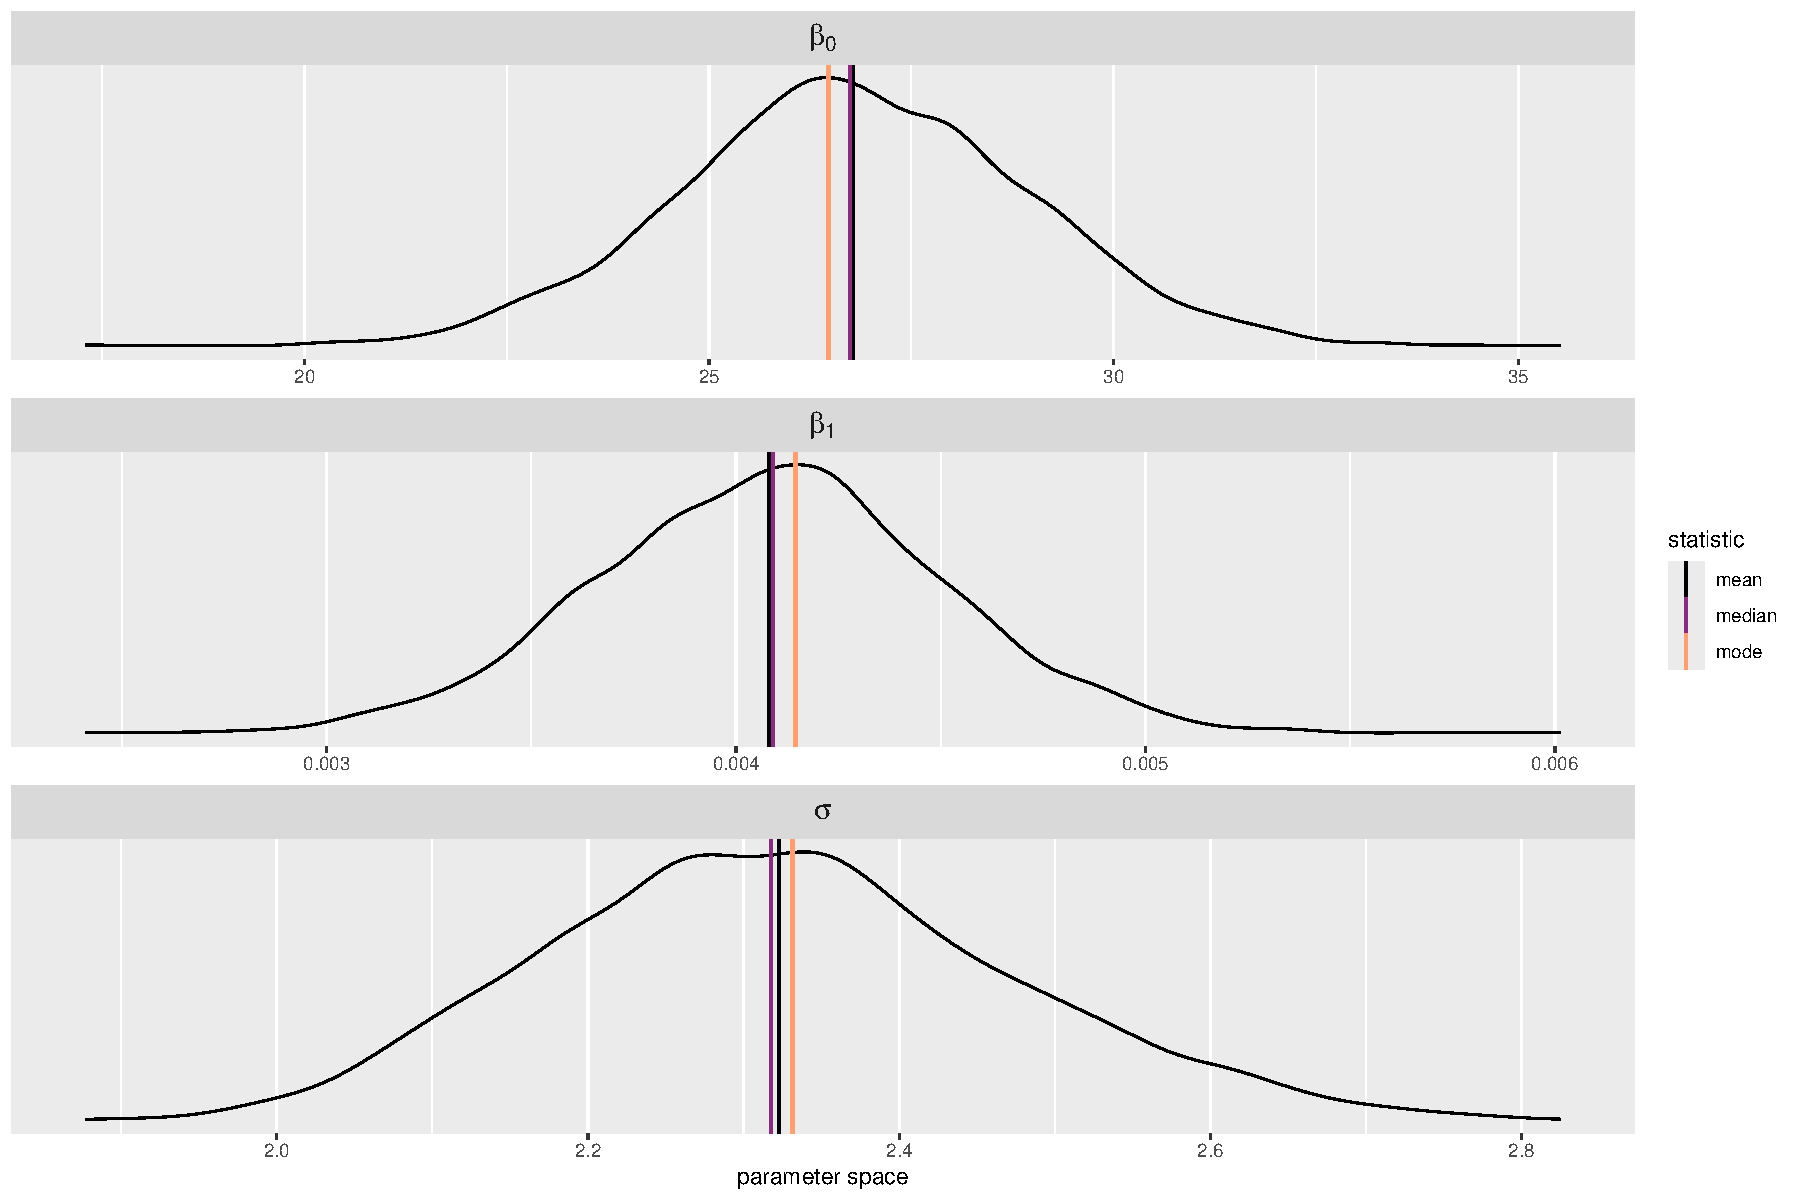
\includegraphics{Bayes_Lab_1_files/figure-pdf/unnamed-chunk-60-2.pdf}

\begin{Shaded}
\begin{Highlighting}[]
\FunctionTok{set.seed}\NormalTok{(}\DecValTok{20}\NormalTok{)}

\NormalTok{draws2 }\SpecialCharTok{\%\textgreater{}\%} 
  \CommentTok{\# take a random sample of 20 rows}
  \FunctionTok{slice\_sample}\NormalTok{(}\AttributeTok{n =} \DecValTok{20}\NormalTok{) }\SpecialCharTok{\%\textgreater{}\%} 
  \FunctionTok{select}\NormalTok{(.draw, beta0, beta1) }\SpecialCharTok{\%\textgreater{}\%} 
  \FunctionTok{expand\_grid}\NormalTok{(}\AttributeTok{body\_mass\_g =} \FunctionTok{range}\NormalTok{(gentoo}\SpecialCharTok{$}\NormalTok{body\_mass\_g, }\AttributeTok{na.rm=}\ConstantTok{TRUE}\NormalTok{)) }\SpecialCharTok{\%\textgreater{}\%} 
  \FunctionTok{mutate}\NormalTok{(}\AttributeTok{y\_hat =}\NormalTok{ beta0 }\SpecialCharTok{+}\NormalTok{ beta1 }\SpecialCharTok{*}\NormalTok{ body\_mass\_g) }\SpecialCharTok{\%\textgreater{}\%} 
  \FunctionTok{ggplot}\NormalTok{(}\FunctionTok{aes}\NormalTok{(}\AttributeTok{x =}\NormalTok{ body\_mass\_g, }\AttributeTok{y =}\NormalTok{ y\_hat, }\AttributeTok{group =}\NormalTok{ .draw, }\AttributeTok{color =}\NormalTok{ beta0)) }\SpecialCharTok{+}
  \FunctionTok{geom\_line}\NormalTok{() }\SpecialCharTok{+}
  \FunctionTok{scale\_color\_viridis\_c}\NormalTok{(}\FunctionTok{expression}\NormalTok{(beta[}\DecValTok{0}\NormalTok{]}\SpecialCharTok{\textasciitilde{}}\NormalTok{(the}\SpecialCharTok{\textasciitilde{}}\NormalTok{intercept)), }\AttributeTok{end =}\NormalTok{ .}\DecValTok{9}\NormalTok{)}
\end{Highlighting}
\end{Shaded}

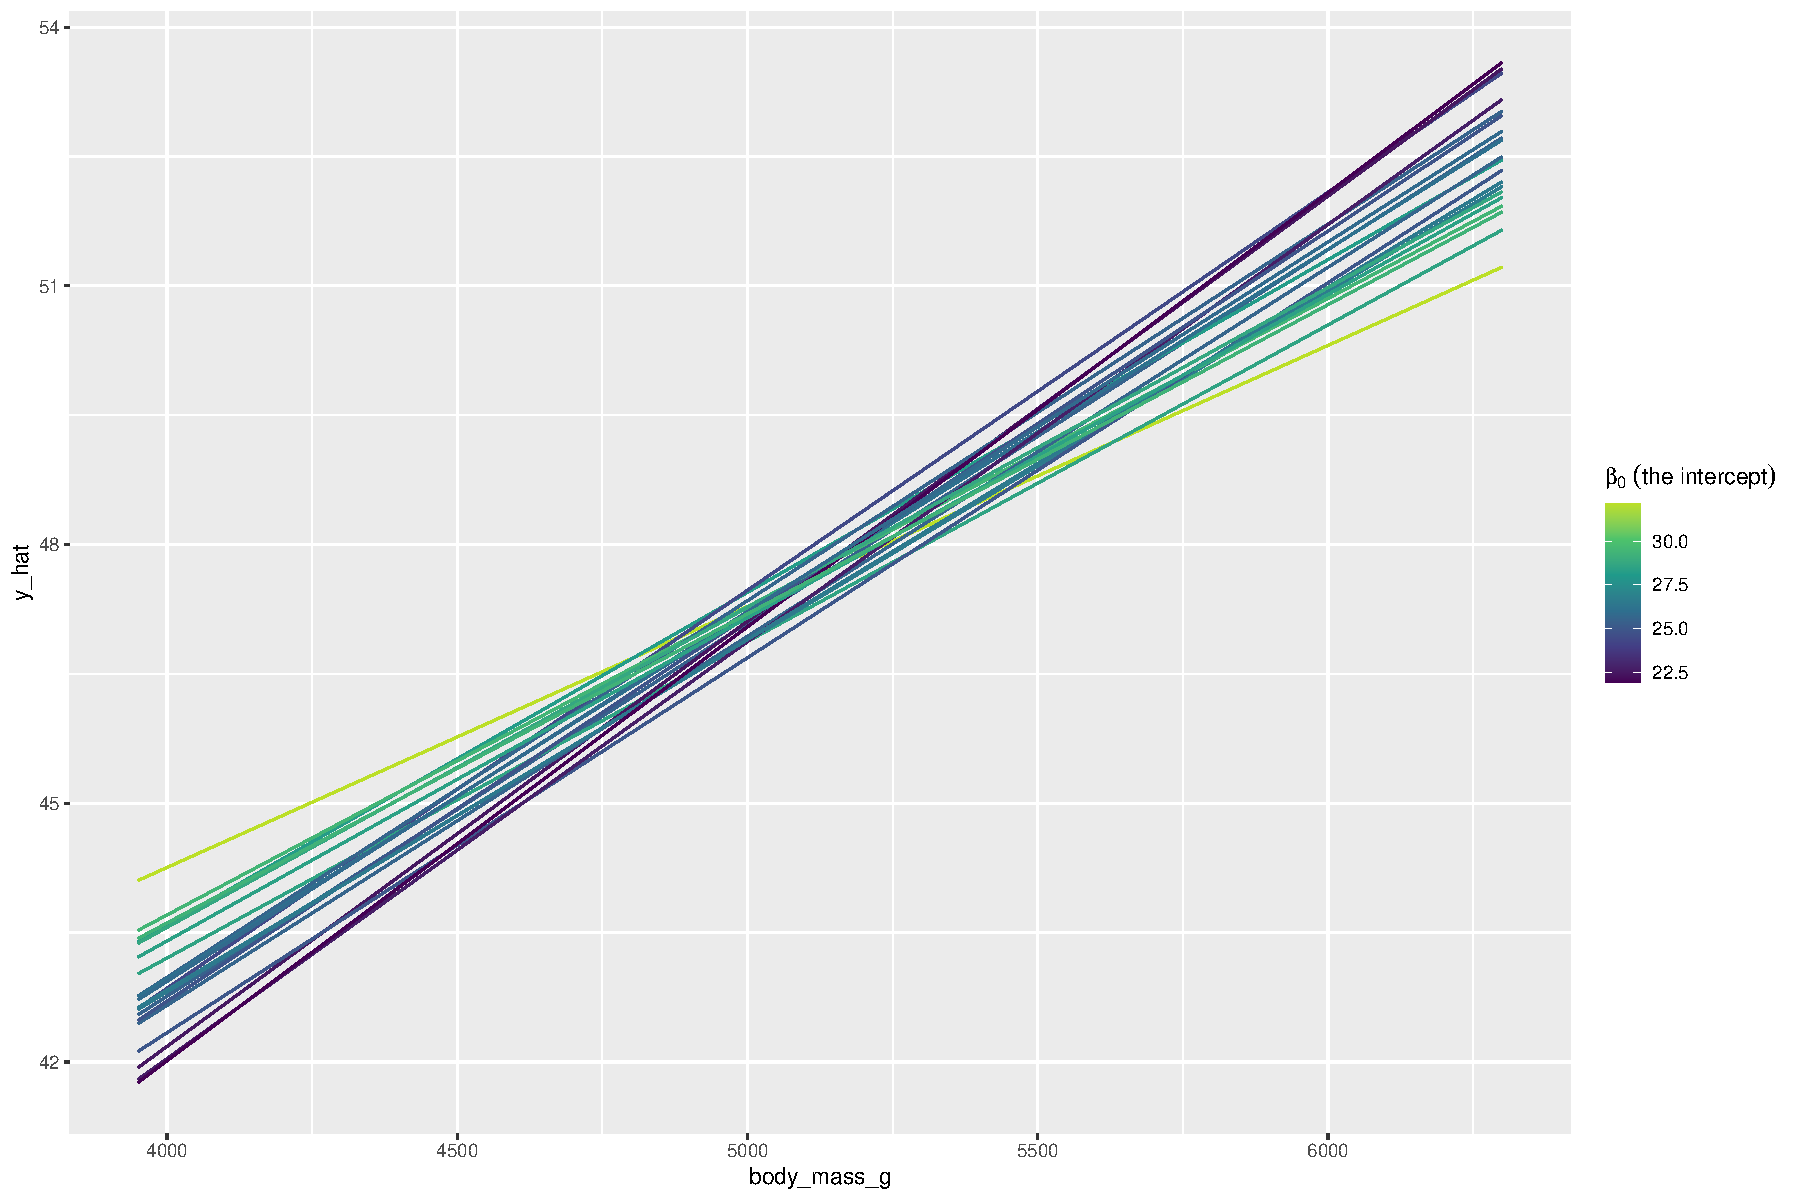
\includegraphics{Bayes_Lab_1_files/figure-pdf/unnamed-chunk-60-3.pdf}

\subsection{References}\label{references}

Gelman, A., Hill, J., \& Vehtari, A. (2020). \emph{Regression and other
stories}. Cambridge University Press.
https://doi.org/10.1017/9781139161879

Kruschke, J. K. (2015). \emph{Doing Bayesian data analysis: A tutorial
with R, JAGS, and Stan}. Academic Press.
https://sites.google.com/site/doingbayesiandataanalysis/

McElreath, R. (2020). \emph{Statistical rethinking: A Bayesian course
with examples in R and Stan} (Second Edition). CRC Press.
https://xcelab.net/rm/statistical-rethinking/

McElreath, R. (2015). \emph{Statistical rethinking: A Bayesian course
with examples in R and Stan}. CRC press.
https://xcelab.net/rm/statistical-rethinking/

\subsection{Session information}\label{session-information}

\begin{Shaded}
\begin{Highlighting}[]
\FunctionTok{sessionInfo}\NormalTok{()}
\end{Highlighting}
\end{Shaded}

\begin{verbatim}
R version 4.4.1 (2024-06-14)
Platform: x86_64-apple-darwin20
Running under: macOS 15.4

Matrix products: default
BLAS:   /Library/Frameworks/R.framework/Versions/4.4-x86_64/Resources/lib/libRblas.0.dylib 
LAPACK: /Library/Frameworks/R.framework/Versions/4.4-x86_64/Resources/lib/libRlapack.dylib;  LAPACK version 3.12.0

locale:
[1] en_US.UTF-8/en_US.UTF-8/en_US.UTF-8/C/en_US.UTF-8/en_US.UTF-8

time zone: America/New_York
tzcode source: internal

attached base packages:
[1] stats     graphics  grDevices datasets  utils     methods   base     

other attached packages:
 [1] ggdist_3.3.2        broom.mixed_0.2.9.6 broom_1.0.7        
 [4] brms_2.22.0         Rcpp_1.0.14         ggside_0.3.1       
 [7] lubridate_1.9.4     forcats_1.0.0       stringr_1.5.1      
[10] dplyr_1.1.4         purrr_1.0.4         readr_2.1.5        
[13] tidyr_1.3.1         tibble_3.2.1        ggplot2_3.5.1      
[16] tidyverse_2.0.0    

loaded via a namespace (and not attached):
 [1] tidyselect_1.2.1     viridisLite_0.4.2    farver_2.1.2        
 [4] loo_2.8.0            fastmap_1.2.0        tensorA_0.36.2.1    
 [7] digest_0.6.37        estimability_1.5.1   timechange_0.3.0    
[10] lifecycle_1.0.4      StanHeaders_2.32.10  processx_3.8.5      
[13] magrittr_2.0.3       posterior_1.6.0      compiler_4.4.1      
[16] rlang_1.1.4          tools_4.4.1          utf8_1.2.4          
[19] yaml_2.3.10          knitr_1.49           labeling_0.4.3      
[22] bridgesampling_1.1-2 curl_6.2.0           pkgbuild_1.4.6      
[25] plyr_1.8.9           abind_1.4-8          withr_3.0.2         
[28] grid_4.4.1           stats4_4.4.1         xtable_1.8-4        
[31] colorspace_2.1-1     future_1.34.0        inline_0.3.21       
[34] emmeans_1.10.7       globals_0.16.3       scales_1.3.0        
[37] cli_3.6.3            mvtnorm_1.3-3        rmarkdown_2.28      
[40] generics_0.1.3       RcppParallel_5.1.10  rstudioapi_0.17.1   
[43] reshape2_1.4.4       tzdb_0.4.0           rstan_2.32.6        
[46] splines_4.4.1        bayesplot_1.11.1     parallel_4.4.1      
[49] matrixStats_1.5.0    vctrs_0.6.5          V8_6.0.3            
[52] Matrix_1.7-0         jsonlite_1.8.8       callr_3.7.6         
[55] hms_1.1.3            listenv_0.9.1        glue_1.8.0          
[58] parallelly_1.42.0    ps_1.9.0             codetools_0.2-20    
[61] distributional_0.5.0 stringi_1.8.4        gtable_0.3.6        
[64] QuickJSR_1.5.2       palmerpenguins_0.1.1 munsell_0.5.1       
[67] pillar_1.10.1        furrr_0.3.1          htmltools_0.5.8.1   
[70] Brobdingnag_1.2-9    R6_2.5.1             evaluate_1.0.3      
[73] lattice_0.22-6       backports_1.5.0      renv_1.0.7          
[76] rstantools_2.4.0     coda_0.19-4.1        gridExtra_2.3       
[79] nlme_3.1-164         checkmate_2.3.2      mgcv_1.9-1          
[82] xfun_0.51            pkgconfig_2.0.3     
\end{verbatim}



\end{document}
